\PassOptionsToPackage{hyperfootnotes=false}{hyperref}
\documentclass[Master,english,IEEE]{twbook}
\usepackage[utf8]{inputenc}
\usepackage[T1]{fontenc}
\usepackage{longtable,booktabs,multirow,calc,etoolbox}
\usepackage{pdflscape}
\usepackage{footnotehyper}
\usepackage{microtype}

\newcommand{\angstrom}{\ensuremath{\text{\AA}}}
\newcounter{tablebeforeaitools}
\makeatletter
\newcommand{\labelcurrenttable}[1]{%
  \phantomsection
  \protected@edef\@currentlabel{\thetable}%
  \label{#1}}
\makeatother
\providecommand{\tightlist}{%
  \setlength{\itemsep}{0pt}\setlength{\parskip}{0pt}}

\degreecourse{Artificial Intelligence Engineering}
\addbibresource{Literatur.bib}
\ExecuteBibliographyOptions{sorting=none}
\DeclareBibliographyDriver{misc}{%
  \printfield{note}%
  \newunit\newblock%
  \printfield{url}%
  \finentry}

\title{Comparative Analysis of Physics-Based and AI-Based Molecular Docking Tools}
\author{Dominik Mann, PhD BSc}
\studentnumber{2410585017}
\supervisor{FH-Prof. Priv.-Doz. Dipl.-Ing.(FH) Dr.\\Bernhard Knapp\\DI Dr. Heinrich Krobath\\Assoz Univ-Prof. DI Dr. Isabella Derler}
\place{Wien}

% Abstract (\outline) and English keywords. The twbook class typesets \outline as an
% "Abstract" chapter on a new page immediately after the Declaration, with the
% \keywords list at the foot of that page. (A German \kurzfassung/\schlagworte pair
% could be added here as well if the examination office requires a bilingual summary.)
\outline{Molecular docking predicts how small-molecule ligands bind their protein
targets, yet physics-based and machine-learning tools embody very different
trade-offs between geometric accuracy and physical realism. This thesis presents a
systematic, reproducible comparison of a physics-based method (AutoDock Vina)
against two AI-based methods --- the diffusion-generative DiffDock and the
E(3)-equivariant regression model EquiBind --- across two complementary settings. A
calibration benchmark of 303 co-crystallised complexes enables ground-truth
assessment of both pose accuracy (heavy-atom RMSD) and physical validity through the
PoseBusters test battery. A crystal-free application to the calcium-release-activated
channel Orai1, using molecular-dynamics receptor snapshots together with experimental
and benchmark ligand sets, probes how the tools behave on a realistic
membrane-protein target without a reference structure.

Across both settings, physical validity --- not RMSD --- is the sharpest
discriminator. AutoDock Vina produces physically valid poses for essentially every
complex (94.8\% of all produced poses), whereas the raw AI outputs are largely
non-physical (23.9\% for DiffDock and 2.7\% for unguided EquiBind). Post-hoc
force-field minimisation is the dominant driver of usability, raising the median
per-complex validity of DiffDock from 13.3\% to roughly 90\% and that of unguided
EquiBind from 0\% to about 57\%, while it cannot recover an unsampled or grossly
misplaced binding mode. Deepening the inspected ranking pool further increases the
recovery of valid, near-native poses. On Orai1 the three tools localise to markedly
different sites, and transmembrane-pore filtering, pose clustering and
protein--ligand interaction-fingerprint analysis quantify their disagreement.
Overall, the results argue for combined accuracy-and-validity criteria and routine
geometry refinement whenever AI-based docking tools are deployed.}

\keywords{Molecular docking; Physics-based versus AI-based methods; PoseBusters
physical validity; Post-hoc pose refinement; Orai1 calcium channel}

\begin{document}

% Cite all sources in their reviewed numeric order before the first body citation.
\nocite{ref001,ref002,ref003,ref004,ref005,ref006,ref007,ref008,ref009,ref010,ref011,ref012,ref013,ref014,ref015,ref016,ref017,ref018,ref019,ref020,ref021,ref022,ref023,ref024,ref025,ref026,ref027,ref028,ref029,ref030,ref031,ref032,ref033,ref034,ref035,ref036,ref037,ref038,ref039,ref040,ref041,ref042,ref043,ref044,ref045,ref046,ref047,ref048,ref049,ref050,ref051,ref052,ref053,ref054,ref055,ref056,ref057,ref058,ref059,ref060,ref061,ref062,ref063,ref064,ref065,ref066,ref067,ref068,ref069,ref070,ref071,ref072}
\maketitle

\hypertarget{motivation}{%
\chapter{\texorpdfstring{Motivation }{Motivation }}\label{motivation}}

Molecular docking is vital in structure-based drug design, predicting the binding modes of small molecules to target proteins and estimating binding affinities. Computationally modelling protein-ligand interactions enables the screening of vast chemical libraries and thus significantly reduces drug development time and costs.

Computational molecular docking emerged in the 1980s from geometric shape-matching methods that predicted ligand binding modes from steric complementarity \cite{ref001}. In 1990, Goodsell and Olson introduced an automated docking procedure based on simulated annealing \cite{ref002}, helping establish the AutoDock family. The combination of empirical interaction models with efficient volumetric energy evaluation enabled flexible-ligand conformational search and increasingly large virtual screens \cite{ref003}. HADDOCK later extended data-guided docking to flexible, multistage modelling of biomolecular complexes \cite{ref004}, \cite{ref005}. These classical approaches remain influential because their search and scoring procedures are explicit, reproducible and continuously maintained.

AI-enabled protein-ligand docking methods have proliferated in recent years \cite{ref006}, \cite{ref007}. DiffDock and EquiBind are prominent examples. DiffDock formulates docking as equivariant diffusion \cite{ref024}, whereas EquiBind uses geometric deep learning for direct pose regression \cite{ref010}. Despite reported gains in speed or accuracy, comparisons between classical and AI-based docking often focus on selected output poses, use unequal search conditions or omit post-docking optimisation and explicit physical-validity screening \cite{ref011,ref012,ref013}, \cite{ref035}. The following research questions therefore guide this thesis.

\begin{enumerate}
\item[\textbf{RQ1}] How do the quality and stability of poses predicted by AutoDock Vina, DiffDock and EquiBind differ?
\item[\textbf{RQ2}] How does post-docking optimisation affect the quality and stability of predicted poses?
\item[\textbf{RQ3}] How computationally efficient are physics-based and AI-based docking approaches?
\item[\textbf{RQ4}] What opportunities and limitations do physics-based and AI-based docking tools present?
\end{enumerate}

\hypertarget{literature-review}{%
\chapter{\texorpdfstring{Literature Review }{Literature Review }}\label{literature-review}}

\hypertarget{molecular-docking-process}{%
\section{Molecular Docking Process}\label{molecular-docking-process}}

Molecular docking aims to predict geometry, bound pose and interactions of small-molecule ligands and target proteins. Ligands can be molecules, ions, peptides or proteins that bind to larger biomolecules to form complexes that serve biological functions. Ligands can be substrates that enzymes act upon, inhibitors that block enzyme activity, activators that enhance function, signalling molecules like neurotransmitters, or ions essential for structural or catalytic roles \cite{ref016}. When docking, ligands often induce conformational changes in the protein, altering its functional state and triggering downstream biological effects \cite{ref016}.

Proteins are amino-acid sequences that fold into three-dimensional structures whose shapes support functions such as catalysis, structural organisation and cellular signalling. Small-molecule binding at protein pockets can modulate these functions, which makes proteins central targets in drug discovery \cite{ref014}, \cite{ref015}.

\hypertarget{physics-based-molecular-docking}{%
\subsection{Physics-Based Molecular Docking}\label{physics-based-molecular-docking}}

Physics-based protein-ligand docking is a computational process that predicts how ligands (small molecules) bind to proteins at the atomic level. This prediction is vital for understanding molecular recognition mechanisms. Next to predicting ligand conformation and position (sampling), binding affinities are assessed (scoring) in the docking process. The classical workflow proceeds in five stages and is in detail described in Figure~\ref{fig:literature-docking-workflow}.

\begin{figure}[!htbp]
\centering
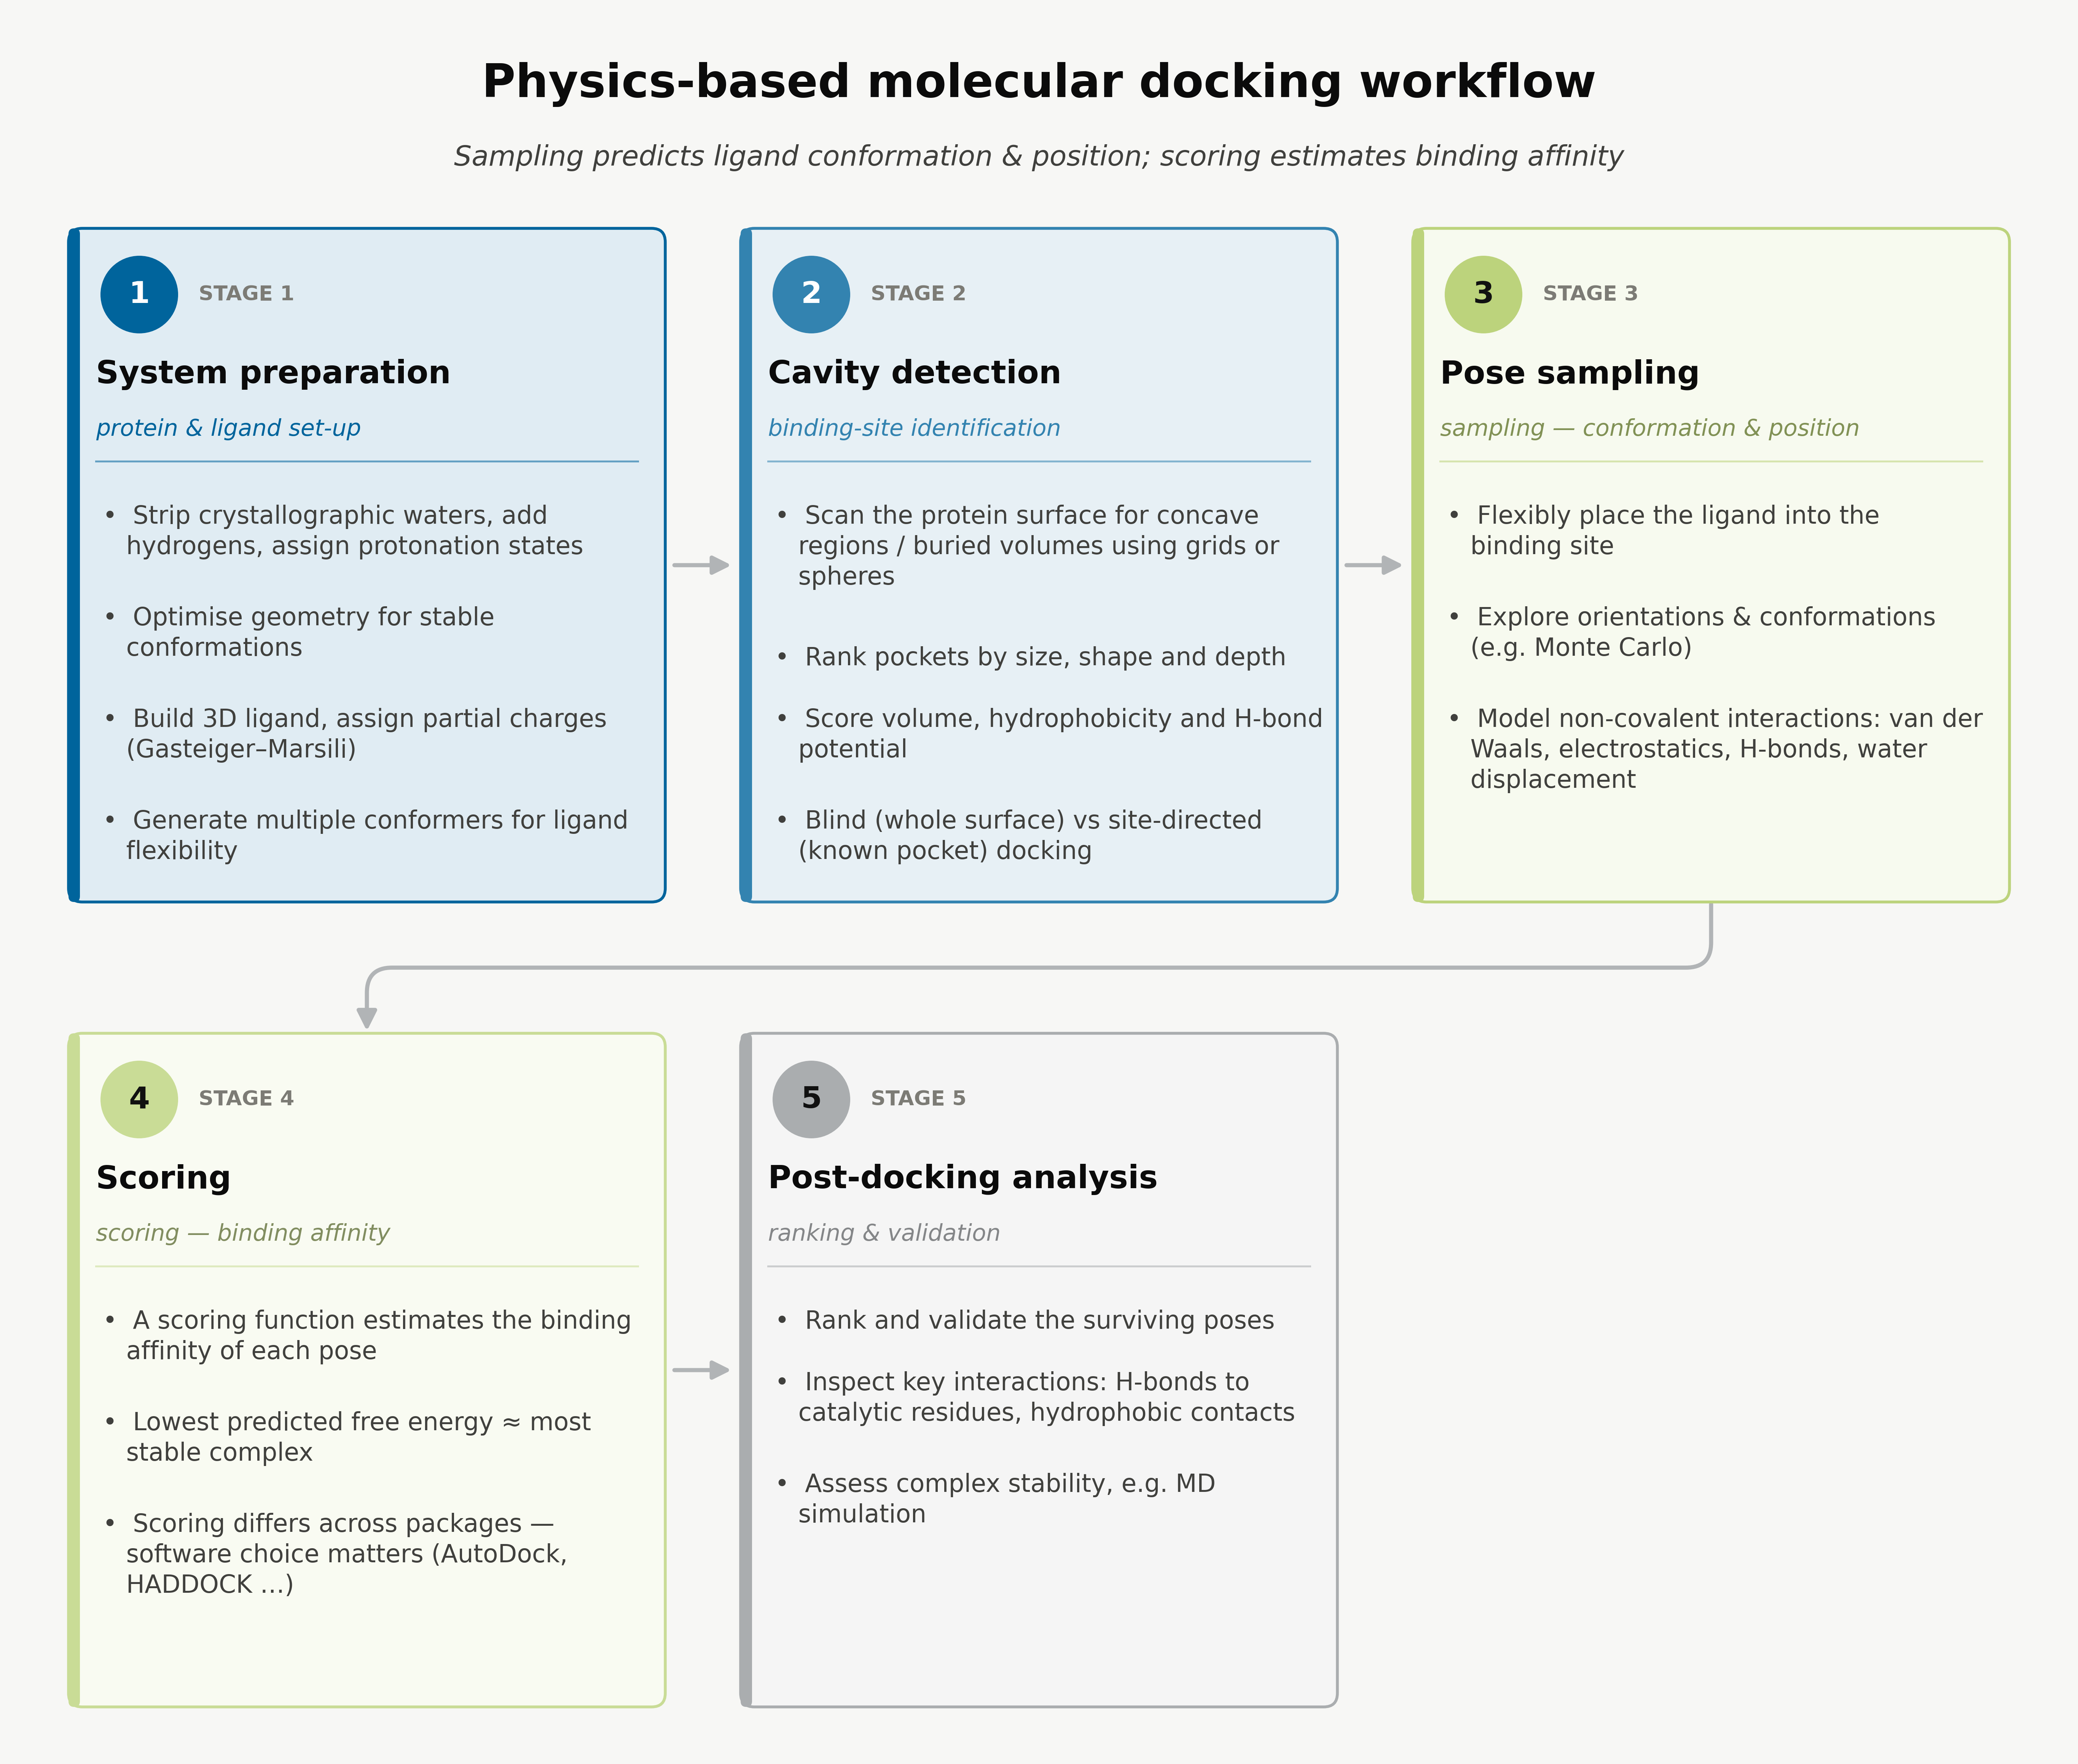
\includegraphics[width=\linewidth,height=0.78\textheight,keepaspectratio]{media/media/image1.png}
\caption{Physics-based Docking Flow Chart (\cite{ref015}, \cite{ref017}, \cite{ref018}, \cite{ref019}, \cite{ref020}, \cite{ref021})}\label{fig:literature-docking-workflow}
\end{figure}

\hypertarget{autodock-vina}{%
\subsubsection{AutoDock Vina}\label{autodock-vina}}

AutoDock Vina is a physics-based docking tool combining an empirical scoring function with an efficient global optimisation strategy \cite{ref022}. After receptor and ligand preparation, it generates random poses inside a user-defined search box and refines them by iterated local search, namely random perturbation followed by gradient-based local optimisation with a BFGS-like quasi-Newton method over precomputed interaction grids. Similar poses are clustered by RMSD and the lowest-energy representatives are returned \cite{ref023}. The scoring function expresses the predicted binding free energy as a weighted sum of pairwise atom-type terms over the surface distance between atoms, namely two attractive Gaussian steric terms, a repulsive parabola, a hydrophobic term and a hydrogen-bond term, divided by a factor growing with the number of rotatable bonds as a flexibility penalty. Its six weights were fixed once by non-linear regression against the PDBbind set, giving Vina a hybrid empirical and knowledge-based character \cite{ref022}. Because the score is evaluated together with its gradient, each pose is minimised during the search, so no separate post-docking optimisation is needed. The full protocol, scoring equations and fitted weights are reproduced in the Appendix (Tools and Functions, AutoDock Vina).

\hypertarget{ai-based-molecular-docking}{%
\subsection{AI-Based Molecular Docking}\label{ai-based-molecular-docking}}

AI-based molecular docking tools employ diverse computational strategies. Common strategies include deep-learning neural networks that predict binding poses directly from protein and ligand structures, diffusion models like DiffDock \cite{ref024} that treat docking as a generative sampling problem, geometric deep learning approaches such as EquiBind \cite{ref009}, \cite{ref010} and TankBind \cite{ref025}, \cite{ref026} that use SE(3)-equivariant networks, and regression-based models like KarmaDock \cite{ref027} and GAABind \cite{ref028} that predict binding affinities or poses with learned scoring functions. Other notable AI-based algorithms include SurfDock, DiffBindFR, DynamicBind, QuickBind, and hybrid methods like Interformer, which integrate traditional conformational searches with AI-driven scoring functions. Some methods, such as DeepDock and Uni-Mol, perform "blind docking" without requiring predefined binding sites, while others, like co-folding models, simultaneously predict structural changes in both protein and ligand to account for flexibility \cite{ref013}, \cite{ref029}.

In contrast to traditional exhaustive conformational search algorithms and empirical scoring functions, AI-based tools learn complex interaction patterns from large datasets of protein-ligand complexes to directly predict optimal binding conformations. Moreover, AI-based methods tend to be computationally efficient, which improves scalability for large-scale virtual screening.

\hypertarget{diffdock}{%
\subsubsection{DiffDock}\label{diffdock}}

DiffDock is a diffusion generative model that treats pose prediction as a generative task rather than optimisation of a hand-crafted energy function \cite{ref024}. Protein and ligand are represented as graphs, and the ligand pose is parameterised by translation, rotation and internal torsion angles. During training a forward process corrupts known poses by adding noise to these variables, and at inference the reverse process starts from random placements and denoises them over several steps, where an SE(3)-equivariant neural network predicts updates that move the pose toward a high-probability bound conformation. The equivariance keeps predictions consistent under rigid motions of the coordinates. Because sampling is stochastic, DiffDock returns several plausible poses, which suits multimodal docking landscapes. Its scoring has two learned components, namely a diffusion score model that steers the denoising trajectory and a confidence model that ranks poses by predicted correctness, that is whether a pose falls below a 2\angstrom{} RMSD threshold rather than an affinity-like energy. These criteria live implicitly in the network weights, so performance depends heavily on the training data and confidence-model calibration \cite{ref024}. Full details are given in the Appendix (Tools and Functions, DiffDock).

\hypertarget{equibind}{%
\subsubsection{EquiBind}\label{equibind}}

EquiBind is a direct geometric deep-learning approach to blind docking predicting the bound pose directly in a single forward pass of an SE(3)-equivariant neural network. Protein and ligand are encoded as graphs, and interaction-aware equivariant message passing between them lets ligand atoms attend to the most relevant protein regions, so the network infers both where the ligand binds and how it is oriented without a predefined site. Its central mechanism is the prediction of matching key points on the ligand and the protein surface, after which the best rigid-body transformation is computed by a singular-value-decomposition (Kabsch-style) step that places the ligand into the pocket, followed by a conformer-fitting stage that adjusts torsions. EquiBind uses no separate scoring function at inference, and is instead trained with losses that penalise the geometric error to the experimental reference, namely ligand RMSD-type, alignment and region losses, so the ranking rule is internalised during training and no affinity-like number is produced. Dropping both stochastic search and repeated denoising gives it a large runtime advantage for high-throughput docking. Full details are given in the Appendix (Tools and Functions, EquiBind).

\hypertarget{optimization-tools}{%
\subsection{Optimization Tools}\label{optimization-tools}}

\hypertarget{smina}{%
\subsubsection{smina}\label{smina}}

Unlike the tools above, smina and gnina are used here as lightweight refinement tools that re-score and locally optimise generated poses. smina is a fork of AutoDock Vina developed by Koes et al. \cite{ref055}. It inherits Vina\textquotesingle s empirical scoring function and search machinery unchanged but re-implements them so that individual energy terms can be reweighted or swapped and custom atom types defined. The energy it optimises is therefore the Vina objective itself, namely the weighted sum of two Gaussian steric terms, a steric-repulsion penalty, a hydrophobic contact term and a hydrogen-bond term, divided by a factor growing with the number of rotatable bonds, the same function described above. Beyond full docking, smina exposes a fast local-minimisation mode that relaxes a supplied pose into the nearest energy minimum by gradient-based optimisation without repeating the conformational search. This makes it well suited to post-docking optimisation, since a pose seated in roughly the correct pocket but clashing with the receptor can be minimised against the Vina function, removing the clash while leaving the placement essentially unchanged \cite{ref057}.

\hypertarget{gnina}{%
\subsubsection{gnina}\label{gnina}}

Because gnina is a fork of smina, both share the docking algorithm inherited from Vina \cite{ref056}, \cite{ref067}, \cite{ref068}. Sampling uses Markov-chain Monte Carlo chains that apply random rigid-body and torsional perturbations, drive each candidate to a local minimum of the Vina energy by quasi-Newton minimisation, and accept or reject it by a Metropolis criterion, so the Vina energy is the quantity optimised during search. gnina differs in ranking, replacing the hand-crafted score with a learned one. An ensemble of convolutional neural networks rescores the poses, each reading a three-dimensional grid of Gaussian atom-type densities built with libmolgrid and trained on two objectives, namely a cross-entropy classifier predicting the probability a pose lies within 2\angstrom{} RMSD of the native mode (CNNscore) and a hinged regression head predicting a binding constant on a pK scale (CNNaffinity). Their product CNN\_VS is preferred for virtual screening \cite{ref068}, and these learned criteria are applied to already-minimised poses rather than being analytic energies. gnina therefore couples a physics-based sampler to a deep-learning scoring function and is used here purely for model-agnostic rescoring and refinement \cite{ref058}. Full details appear in the Appendix (Tools and Functions, Optimization Tools).

\hypertarget{comparisons-of-physics-based-and-ai-based-molecular-docking}{%
\subsection{Comparisons of Physics-Based and AI-Based Molecular Docking}\label{comparisons-of-physics-based-and-ai-based-molecular-docking}}

The rapid emergence of AI-based molecular docking tools, which promise computationally efficient and reliable binding predictions, has drawn the attention of scholars and practitioners alike. New tools are usually released with a peer- or non-peer-reviewed paper setting out their advantages and disadvantages, and independent researchers have since compared different tools across diverse datasets. As evident from Table~\ref{tab:literature-comparisons}, a wide range of tools using a converging set of metrics for comparison were compared.

\begin{longtable}[]{@{}
  >{\raggedright\arraybackslash}p{(\columnwidth - 6\tabcolsep) * \real{0.1041}}
  >{\raggedright\arraybackslash}p{(\columnwidth - 6\tabcolsep) * \real{0.3676}}
  >{\raggedright\arraybackslash}p{(\columnwidth - 6\tabcolsep) * \real{0.2287}}
  >{\raggedright\arraybackslash}p{(\columnwidth - 6\tabcolsep) * \real{0.2996}}@{}}
\caption{Physics-Based and AI-Based Docking Studies}\tabularnewline
\toprule\noalign{}
{\raggedright \textbf{Study (Year)}} & \centering\arraybackslash\textbf{Docking Tools Compared} & \centering\arraybackslash\textbf{Datasets Used} & \centering\arraybackslash\textbf{Metrics for Comparison} \\
\midrule\noalign{}
\endfirsthead
\caption[]{Physics-Based and AI-Based Docking Studies (continued)}\tabularnewline

\toprule\noalign{}
{\raggedright \textbf{Study (Year)}} & \centering\arraybackslash\textbf{Docking Tools Compared} & \centering\arraybackslash\textbf{Datasets Used} & \centering\arraybackslash\textbf{Metrics for Comparison} \\
\midrule\noalign{}
\endhead
\bottomrule\noalign{}
\endlastfoot
Li et al. (2025) \cite{ref013} & Glide SP, AutoDock Vina (physics-based); SurfDock, DiffBindFR, DynamicBind (generative diffusion); KarmaDock, GAABind, QuickBind (regression-based AI); Interformer (hybrid) & Astex Diverse Set, PoseBusters Benchmark, DockGen (pose/validity); DEKOIS2.0, DUD-E (virtual screening) & RMSD (pose accuracy), PB-valid (physical plausibility), Interaction Recovery, ROC-AUC, EF0.5\%, BEDROC (VS), Generalization (protein/ligand/pocket similarity) \\
Jiang et al. (2025) \cite{ref012} & Glide, AutoDock Vina, MOE, Discovery Studio ( physics-based ); Uni-Mol, DiffDock, SurfDock, Interformer, EquiBind, FABind, DeepDock, TankBind (AI); AlphaFold3, Boltz-1, Chai-1 (AI co-folding) & PoseX-SD (self-docking), PoseX-CD (cross-docking), Astex & RMSD, Success Rate, Physical Validity, Generalization, Leaderboard Ranking \\
Gu et al. (2025) \cite{ref032} & Glide, AutoDock Vina ( physics-based ); KarmaDock, CarsiDock, RTMScore (AI/ML scoring) & TrueDecoy, RandomDecoy & RMSD, Physical Validity, VS Enrichment, ROC-AUC \\
Schaller et al. (2024) \cite{ref033} & Fred, Hybrid, Posit, AutoDock Vina, PLANTS ( physics-based ); CNN-Score, RF-Score-VS, gnina (ML scoring) & Kinase structures/ligands, DUD-E & RMSD, Success Rate, VS Enrichment, ROC-AUC \\
\end{longtable}
\labelcurrenttable{tab:literature-comparisons}

Recent evaluations show that learned docking models remain sensitive to physical validity and structural novelty \cite{ref013}. None of the cited studies evaluates Orai1, so AutoDock Vina is retained as an established baseline rather than assumed to be universally superior.

\hypertarget{methods}{%
\chapter{\texorpdfstring{Methods }{Methods }}\label{methods}}

The methodological premise of this work is exploratory rather than confirmatory. Instead of committing to a single docking engine, it deliberately combines a physics-based method (AutoDock Vina) with two complementary AI-based methods, the diffusion model DiffDock and the regression model EquiBind, and couples each deep-learning method to a lightweight physics-based refinement step (smina/gnina). Mapping where each toolchain performs well, and testing whether their union covers more of the benchmark than any single tool, provides the ground for the docking of the reference-free Orai1 target.

The comparison rests on a small set of measures applied identically to every tool. Geometric accuracy is the symmetry-corrected heavy-atom RMSD of a docked pose to the crystal ligand, with the conventional success threshold of RMSD \ensuremath{\leq} 2\angstrom{}. This in-place RMSD is further decomposed into a shape and a position component through the exact identity in-place\textsuperscript{2} = placement\textsuperscript{2} + form\textsuperscript{2}. The form error is the best-fit (Kabsch) RMSD that remains once translation and rotation are removed and the placement error is the positional remainder, with a pose judged form-correct when its form error is at most 1\angstrom{}. The decomposition separates a distorted ligand conformation from a merely mis-positioned one, since only a conformationally faithful pose can present its pharmacophore correctly and reproduce the native interaction pattern.

Physical plausibility is further assessed with the PoseBusters battery, which flags chemically or sterically impossible poses (PB-valid). Because a pose can be geometrically close yet physically broken, the two are combined into a single usable-pose criterion, namely RMSD \ensuremath{\leq} 2\angstrom{} and PB-valid, which serves as the primary metric. These are further resolved by pose ranking (the ranked or scored top-1 pose versus the best or oracle pose that is closest placed to the crystal ligand) and, for the binding-site question, by cross-tool clustering of the docked poses against the crystallographic pocket.

\hypertarget{datasets}{%
\section{Datasets}\label{datasets}}

Validating the reliability of produced poses by AutoDock Vina, DiffDock and EquiBind required the careful selection of an experimentally validated dataset as ground truth. A reliable dataset provides protein and ligand complexes across a wide range of chemical scaffolds, sizes and structural classes.

\protect\hypertarget{_Toc235735885}{}{}

\hypertarget{calibration-dataset}{%
\subsection{Calibration Dataset}\label{calibration-dataset}}

% REVIEW QUERY: Please document the identities and exclusion reasons for the five source complexes not included in the 303-case shared analysis, and for the ten further cases without comparable timing records.
The calibration dataset is derived from the 308 high-resolution protein-ligand crystal complexes assembled for the PoseBusters benchmark \cite{ref035}. The shared comparative analysis retained 303 complexes after preparation and processing, while the timing comparison used the 293 cases with comparable timing records. The post-2021 release criterion reduces direct temporal overlap with the published training data of early AI docking models, but it does not exclude homologous proteins, similar ligands or familiar binding pockets. For each retained entry, the cognate ligand is re-docked into its experimentally determined receptor and compared with the crystallographic binding mode. The source set spans a broad range of chemical and structural properties (Table~\ref{tab:methods-calibration-characteristics}). A detailed description of the dataset is provided in Appendix \ref{dataset}.

\begin{longtable}[]{@{}
  >{\raggedright\arraybackslash}p{(\columnwidth - 6\tabcolsep) * \real{0.3528}}
  >{\raggedleft\arraybackslash}p{(\columnwidth - 6\tabcolsep) * \real{0.1472}}
  >{\centering\arraybackslash}p{(\columnwidth - 6\tabcolsep) * \real{0.2500}}
  >{\centering\arraybackslash}p{(\columnwidth - 6\tabcolsep) * \real{0.2500}}@{}}
\caption{Key Characteristics of the Calibration Benchmark Set}\tabularnewline
\toprule\noalign{}
{\raggedright \textbf{Descriptor}} & \centering\arraybackslash\textbf{Median} & \centering\arraybackslash\textbf{IQR (25--75\,\%)} & \centering\arraybackslash\textbf{Range (min--max)} \\
\midrule\noalign{}
\endfirsthead
\caption[]{Key Characteristics of the Calibration Benchmark Set (continued)}\tabularnewline

\toprule\noalign{}
{\raggedright \textbf{Descriptor}} & \centering\arraybackslash\textbf{Median} & \centering\arraybackslash\textbf{IQR (25--75\,\%)} & \centering\arraybackslash\textbf{Range (min--max)} \\
\midrule\noalign{}
\endhead
\bottomrule\noalign{}
\endlastfoot
Heavy atoms & 24 & 16--32 & 6--64 \\
Molecular weight (Da) & 359 & 236--462 & 100--872 \\
Rotatable bonds & 5 & 2--7 & 0--20 \\
H-bond acceptors & 6 & 3--9 & 0--21 \\
H-bond donors & 3 & 2--5 & 0--13 \\
TPSA (\angstrom{}\textsuperscript{2}) & 107 & 66--160 & 0--384 \\
cLogP & 0.9 & \ensuremath{-}1.6--3.2 & \ensuremath{-}8.4--14.0 \\
Fraction sp\textsuperscript{3} C & 0.41 & 0.23--0.57 & 0.00--1.00 \\
QED & 0.44 & 0.29--0.60 & 0.04--0.91 \\
Ring count & 3 & 1--4 & 0--8 \\
\end{longtable}
\labelcurrenttable{tab:methods-calibration-characteristics}

\hypertarget{experimental-dataset}{%
\subsection{Experimental Dataset}\label{experimental-dataset}}

The experimental dataset is the system that the comparison is ultimately intended to address. Unlike the validation dataset, where a crystallographic pose, i.e. ground-truth, is available for every complex, this set targets the calcium release-activated calcium channel Orai1, a target of genuine pharmacological interest, for which experimentally resolved protein-ligand reference structures are not established, so that the binding mode must be predicted rather than re-docked. It pairs a set of Orai1 conformational snapshots with a chemically diverse selection of Orai1-binding compounds, allowing the three docking tools to be compared on a realistic prediction task once their behaviour has been characterised on the validation dataset.

\begin{longtable}[]{@{}
  >{\raggedright\arraybackslash}p{(\columnwidth - 8\tabcolsep) * \real{0.2587}}
  >{\raggedleft\arraybackslash}p{(\columnwidth - 8\tabcolsep) * \real{0.2391}}
  >{\raggedleft\arraybackslash}p{(\columnwidth - 8\tabcolsep) * \real{0.2394}}
  >{\raggedleft\arraybackslash}p{(\columnwidth - 8\tabcolsep) * \real{0.2391}}
  >{\raggedright\arraybackslash}p{(\columnwidth - 8\tabcolsep) * \real{0.0238}}@{}}
\caption[Experimental Orai1 ligands]{Experimental Orai1 ligands. Proposed binding sites are model-derived (mutagenesis, docking, molecular dynamics) and filter-proximal rather than experimentally resolved ligand-bound poses. No cognate Orai1 complex is resolved for any compound, and the binding site of 2-APB (docked as the neutral form 2abp-NH2) is not experimentally resolved.}\tabularnewline
\toprule\noalign{}
{\raggedright \textbf{Ligand Name}} & \centering\arraybackslash\textbf{2-APB} & \centering\arraybackslash\textbf{GSK-7975A} & \centering\arraybackslash\textbf{Synta-66} & {} \\
\midrule\noalign{}
\endfirsthead
\caption[]{Experimental Orai1 Ligands (continued)}\tabularnewline
\toprule\noalign{}
{\raggedright \textbf{Ligand Name}} & \centering\arraybackslash\textbf{2-APB} & \centering\arraybackslash\textbf{GSK-7975A} & \centering\arraybackslash\textbf{Synta-66} & {} \\
\midrule\noalign{}
\endhead
\bottomrule\noalign{}
\endlastfoot
\textbf{Molecular Formula} & C\textsubscript{14}H\textsubscript{16}BNO & C\textsubscript{18}H\textsubscript{12}F\textsubscript{5}N\textsubscript{3}O\textsubscript{2} & C\textsubscript{20}H\textsubscript{17}FN\textsubscript{2}O\textsubscript{3} & \\
\textbf{Molecular Weight (Da)} & 225.1 & 397.3 & 352.4 & \\
\textbf{Heavy Atom Count} & 17 & 28 & 26 & \\
\textbf{Rotatable Bonds} & 6 & 5 & 7 & \\
\textbf{Aromatic Rings} & 2 & 3 & 3 & \\
\textbf{Docked protonation} & neutral & deprotonated (--1) & neutral & \\
\textbf{IC50 uM} & 4 & 4.1 & 2 & \\
\textbf{IC50 Range uM} & 3.0-5.0 & 4.0-4.2 & 1.0-3.0 & \\
\textbf{pIC50} & 5.4 & 5.39 & 5.7 & \\
\textbf{ORAI1 IC50 uM} & 4 & 4.1 & 2 & \\
\textbf{Primary Mechanism} & Bimodal modulator (pore, STIM1) & Extracellular pore blocker & Extracellular pore blocker & \\
\textbf{Proposed Site} & Not experimentally resolved for 2-APB \cite{ref039}, \cite{ref040} & Putative selectivity-filter (E106), direct or allosteric \cite{ref070}, \cite{ref041} & Proposed extracellular TM1/TM3, loops 1/3 \cite{ref071} & \\
\textbf{Site Evidence} & Functional (native 2-APB); site not resolved & Mutagenesis; pore-geometry dependent & Docking, MD, mutagenesis & \\
\end{longtable}
\labelcurrenttable{tab:methods-experimental-ligands}

Limited receptor flexibility was represented with four supplied Orai1 molecular-dynamics snapshots, namely Fr0, Fr300, Fr400 and Fr499 \cite{ref038}, \cite{ref072}. Protonation states were prepared for pH 7.0 using the stated Poisson-Boltzmann and Monte Carlo workflow. The selected ligands were treated consistently under the same preparation protocol. GSK-7975A was docked in its deprotonated (anionic) form. The descriptors above give its neutral reference (C\textsubscript{18}H\textsubscript{12}F\textsubscript{5}N\textsubscript{3}O\textsubscript{2}, 397.3~Da), while the as-docked deprotonated descriptors (C\textsubscript{18}H\textsubscript{11}F\textsubscript{5}N\textsubscript{3}O\textsubscript{2}, 396.3~Da) are those tabulated in Table~\ref{tab:appendix-orai-descriptors}. 2-APB and Synta-66 were docked as neutral species.

The experimental ligand set contains three Orai-related chemotypes, namely 2-APB, docked in its neutral protonation state and labelled 2abp-NH2 in the per-compound results tables, together with GSK-7975A \cite{ref041}, \cite{ref070} and Synta-66 \cite{ref071}. The docked structure is native 2-APB (2-aminoethoxydiphenyl borate), so the reported 2-APB pharmacology \cite{ref039}, \cite{ref040} characterises the docked molecule directly. No cognate Orai1 crystal pose is available for any of the docked compounds, so this set supports a reference-free case study rather than a conventional accuracy benchmark.

All three compounds are tool compounds for store-operated calcium entry, that is the STIM1 to Orai1 pathway that opens calcium release-activated calcium channels once the endoplasmic store is depleted, yet they act on it in three different ways, which is what makes the set informative for a docking comparison.

Because the three compounds act at or near the extracellular pore mouth and the selectivity filter rather than in the conduction pathway, a chemically valid pose lodged inside the transmembrane slab is implausible for any of them, which is precisely what the placement criterion used in the results chapter encodes. Their differing scaffolds also load the three docking tools unevenly. The full pharmacology of each compound, namely GSK-7975A, Synta-66 and 2-APB (docked in its neutral form, 2abp-NH2), together with the sites, selectivity liabilities and mechanistic differences that make the biologically defensible region non-identical across the set, is set out in Appendix~\ref{experimental-ligand-pharmacology}.

Molecular docking of each protein with each drug compound yields a set of 12 complexes. Each of these complexes will be modelled with each toolchain to allow the comparison of the produced dockings.

\hypertarget{evaluation-metrics}{%
\section{Evaluation Metrics}\label{evaluation-metrics}}

Assessing generated poses requires three complementary questions. First, is the ligand placed in a receptor region capable of the interactions relevant to the pharmacological hypothesis? Second, does the ligand retain a credible internal conformation and fit within that region? Third, is the resulting protein-ligand complex physically and chemically admissible? The metrics below address placement, form and validity separately before combining them.

\hypertarget{near-nativeness-rmsd-2uxe5}{%
\subsection{Near-Nativeness (RMSD \ensuremath{\leq} 2\angstrom{})}\label{near-nativeness-rmsd-2uxe5}}

The docking results are compared on three primary measures, applied identically to every tool. The first is geometric accuracy. It is the symmetry-corrected heavy-atom root-mean-square deviation (RMSD) between a docked pose and the crystallographic ligand, defined as

\[\text{RMSD=}\sqrt{\frac{\sum_{i = 1}^{N}d_{i}^{\text{2}}}{N}}\]

where N is the number of heavy atoms and d\textsubscript{i} is the Euclidean distance between the i-th pair of corresponding atoms in their docked and crystallographic positions, computed in place without superposing the pose onto the crystal ligand. A pose counts as accurate at the conventional threshold of RMSD \ensuremath{\leq} 2\angstrom{} \cite{ref044}. The symmetry correction matters because many benchmark ligands are wholly or partly symmetric, so a naïve atom mapping would overstate the error. Because a geometrically close pose can still be chemically or sterically impossible, accuracy is paired with physical plausibility assessed by the PoseBusters battery (PB-valid), described below \cite{ref035}.

The two are combined into a single usable-pose criterion, namely RMSD \ensuremath{\leq} 2\angstrom{} and PB-valid, which is the headline metric throughout and separates a pose that merely looks right from one that could be used. The 2\angstrom{} threshold is the established standard in the docking literature and the AutoDock Vina benchmark, keeping the results comparable with published work \cite{ref022}, \cite{ref035}, \cite{ref050}.

Because a tool can generate a near-native pose yet fail to rank it first, accuracy is reported under two selection regimes, namely the realistic top-1 pose and the oracle (best) pose, the most accurate pose anywhere in the tool's output. The gap between them isolates ranking quality from sampling quality and is developed through the per-rank success rate and the cumulative recovery within the first k ranked poses. A single top-1 view would conflate a weak confidence model with weak sampling and systematically understate the deep-learning tools.

Two secondary measures complete the comparison. Binding-site recovery asks the coarser question of whether a tool places the ligand in the correct pocket at all, assessed by clustering the docked poses across tools and against the crystallographic pocket, which is the appropriate resolution for the reference-free Orai1 system. Computational cost is reported as wall-clock time and as core-seconds per usable pose, that is per pose that is PoseBusters-valid and within 2\angstrom{} of the crystal ligand, since practical value for large-scale screening depends on usable poses returned per unit of compute.

\hypertarget{form-kabsch-rmsd-1-uxe5}{%
\subsection{Form (Kabsch RMSD \ensuremath{\leq} 1 \angstrom{})}\label{form-kabsch-rmsd-1-uxe5}}

Geometric accuracy scored as in-place RMSD, the quantity the \ensuremath{\leq} 2\angstrom{} gate uses, conflates two independent errors, namely where the molecule sits and what shape it holds. The exact identity in-place\textsuperscript{2} = placement\textsuperscript{2} + form\textsuperscript{2} separates them, the form error being the best-fit (Kabsch) RMSD that remains once translation and rotation are removed and the placement error the positional remainder. A pose is called form-correct when its form error is \ensuremath{\leq} 1\angstrom{}.

The heavy-atom RMSD remaining after this best fit is the form error, the component of the deviation that no repositioning can remove, that is the discrepancy in the ligand's own three-dimensional shape. With both ligands translated to a common centroid and R the optimal proper rotation from the singular-value decomposition, it is

\[\text{RMSD}_{\text{form}}\text{=}\sqrt{\frac{\sum_{i = 1}^{N}\left\| Rx_{i}\text{-}y_{i} \right\|^{\text{2}}}{N}}\]

where x\textsubscript{i} and y\textsubscript{i} are the centred coordinates of the i-th heavy-atom pair and N the number of heavy atoms. As with the in-place RMSD, the minimisation is taken over the ligand's symmetry-equivalent atom mappings so that chemically equivalent atoms are not spuriously penalised \cite{ref044}, and the value is read from the PoseBusters implementation \cite{ref035}.

% REVIEW QUERY: Confirm from the analysis code that the same symmetry-equivalent atom mapping was retained for in-place and Kabsch form RMSD. Otherwise describe the exact decomposition as approximate.
For a fixed atom correspondence, rigid superposition gives the per-pose decomposition in-place\textsuperscript{2} = placement\textsuperscript{2} + form\textsuperscript{2}, and placement can be derived as \(\sqrt{\text{in-place}^{2}-\text{form}^{2}}\). The reported placement diagnostic assumes that the same symmetry-equivalent atom mapping is retained for the in-place and form terms. Independently minimising the mapping for each term would make the identity approximate rather than exact. Form recovery is reported for PoseBusters-valid outputs independently of the 2 \angstrom{} in-place threshold, and a pose is form-correct at Kabsch RMSD \ensuremath{\leq} 1 \angstrom{}.

This separation matters because binding is mediated by specific directional contacts, namely hydrogen bonds, hydrophobic burial, \ensuremath{\pi}-stacking and salt bridges, whose geometry is set by the ligand's bound conformation, so a pose reproduces the native interaction pattern only if its form is right. Isolating form therefore probes the physical prerequisite for the interactions the docking is meant to predict, and it localises the limiting stage, since a placement-limited pose (right shape, wrong position) implicates pocket targeting while a form-limited pose (wrong conformation) implicates conformer generation or refinement. The tool-by-tool analysis is presented in the Results (Figures~\ref{fig:results-r3} to \ref{fig:results-r11}).

\hypertarget{physical-and-chemical-validity-posebusters-checks}{%
\subsection{Physical and Chemical Validity (PoseBusters Checks)}\label{physical-and-chemical-validity-posebusters-checks}}

Geometric and form closeness to the crystal do not by themselves guarantee that a pose is physically possible, since RMSD alone can be satisfied by chemically distorted or sterically clashing poses, the failure mode the original PoseBusters study attributes to AI-based methods \cite{ref035}. Every pose was therefore run through the PoseBusters ``dock'' battery and is counted PB-valid only if it passes all PoseBusters checks (Table~\ref{tab:appendix-posebusters-checks}).

The checks fall into three groups. The first covers chemical validity and consistency, namely that the molecular formula, bond connectivity and stereochemistry are preserved and that the molecule parses and sanitises cleanly. The second covers intramolecular geometry, namely bond lengths and angles within distance-geometry tolerance, flat aromatic rings and double bonds, absence of internal steric clash and no gross conformational strain. The third covers intermolecular validity against the receptor, namely minimum distances to the protein, to organic and inorganic cofactors and to waters together with the corresponding volume overlaps, so that the ligand neither interpenetrates the receptor nor occupies space already taken. The full list of individual checks and their tolerances is given in the Appendix (Table~\ref{tab:appendix-posebusters-checks}).

\hypertarget{clustering}{%
\subsection{Clustering}\label{clustering}}

Because a predicted pocket from fpocket or P2Rank carries no ligand atoms, the only quantity comparable across docked poses, predicted pockets and the crystallographic site is the three-dimensional centre, so clustering is performed on each pose\textquotesingle s heavy-atom centroid rather than on full-atom RMSD, with RMSD retained as a complementary pose-quality measure. For every complex the centroids of all three tools are pooled into a pairwise Euclidean distance matrix and partitioned by complete-linkage agglomerative clustering cut at 8\angstrom{}, the physical scale of a binding pocket. The number of clusters is discovered rather than fixed and may be one, so a complex on which all three tools genuinely converge is reported as a single site. Complete linkage guarantees that no cluster\textquotesingle s internal spread exceeds 8\angstrom{} and the cut is deterministic. This replaces the earlier silhouette-maximising K-medoids default, which could never return a single cluster and so split converged sites into spurious sub-pockets.

A second, orthogonal partition classifies the same poses by binding mode. Because two poses related by a 180\ensuremath{^\circ} flip share a centroid, a symmetry-aware in-place RMSD, computed without re-superposition so that translation, orientation and conformation fold into a single distance, is clustered at a 2\angstrom{} threshold. The centroid axis answers where a pose sits and the mode axis how it sits, so together they flag when one spatial site conceals several modes. Candidate pockets are then ranked by cross-tool agreement rather than raw pose count, which stops a high-throughput tool from winning a site on pose count alone.

For the reference-free Orai target the same 8\angstrom{} centroid clustering is applied within each MD frame, but because the four snapshots occupy different coordinate systems poses cannot be clustered by absolute position across frames. Each pose is instead represented by the receptor residues within 4\angstrom{} of the ligand, folded over Orai\textquotesingle s six-fold symmetry, and these fingerprints are clustered into channel regions. With no crystal to arbitrate, the consensus site is defined as the geometric median of the per-tool sites, one point per tool.

Cluster quality is assessed on three complementary axes. Silhouette, Calinski-Harabasz, Davies-Bouldin and nearest-cluster separation are defined only for complexes with at least two clusters and are therefore omitted for one-cluster cases. Compactness can be reported for a single cluster, while bootstrap Jaccard overlap and adjusted Rand indices quantify reproducibility under resampling and against independent partitions. Crystal-site recovery is evaluated separately with the prespecified 4 \angstrom{} centroid threshold. The cluster nearest the crystal is not automatically counted as recovered.

\hypertarget{results}{%
\chapter{Results}\label{results}}

\hypertarget{calibration-dataset-1}{%
\section{Calibration Dataset}\label{calibration-dataset-1}}

Of the 308 source benchmark complexes, 303 were retained in the common calibration analysis for AutoDock Vina, DiffDock and EquiBind. Every generated pose was screened with the PoseBusters suite and compared with the crystal reference by symmetry-corrected heavy-atom RMSD and Kabsch RMSD. Pocket-guided EquiBind variants based on fpocket and P2Rank did not improve the main combined endpoint relative to the unguided configuration.

Both learned pipelines were evaluated before and after local optimisation with smina and gnina. For DiffDock, smina produced a slightly higher combined validity-placement-form recovery than gnina in this dataset, although the margin was not statistically detected at either pose or complex level. For unguided EquiBind, gnina produced the higher validity and combined recovery. These are empirical configuration results. The study did not measure optimisation trajectories and therefore does not establish that one refiner is inherently gentler or more aggressive.

Accordingly, the main comparison uses DiffDock + smina and EquiBind + gnina as the primary refined variants, and these names are used throughout the main Results. Appendix analyses that use raw or gnina-optimised DiffDock output identify the variant explicitly. Their values should not be interchanged with the main comparison.

% RESOLVED 2026-07-26: 7,337 is canonical (per_pose_metrics.csv autodock = 7,337 rows; 6,956 PB-valid = 94.8%). 7,407 was the superseded old run (now _obsolete_dock_7407run); Appendix protocol table corrected to 7,337.
\begin{landscape}
\scriptsize
\setlength{\tabcolsep}{2pt}
\begin{longtable}[]{@{}
  >{\raggedright\arraybackslash}p{(\columnwidth - 28\tabcolsep) * \real{0.1150}}
  >{\raggedright\arraybackslash}p{(\columnwidth - 28\tabcolsep) * \real{0.0943}}
  >{\raggedleft\arraybackslash}p{(\columnwidth - 28\tabcolsep) * \real{0.0613}}
  >{\raggedleft\arraybackslash}p{(\columnwidth - 28\tabcolsep) * \real{0.0638}}
  >{\raggedleft\arraybackslash}p{(\columnwidth - 28\tabcolsep) * \real{0.0583}}
  >{\raggedleft\arraybackslash}p{(\columnwidth - 28\tabcolsep) * \real{0.0603}}
  >{\raggedleft\arraybackslash}p{(\columnwidth - 28\tabcolsep) * \real{0.0638}}
  >{\raggedleft\arraybackslash}p{(\columnwidth - 28\tabcolsep) * \real{0.0583}}
  >{\raggedleft\arraybackslash}p{(\columnwidth - 28\tabcolsep) * \real{0.0603}}
  >{\raggedleft\arraybackslash}p{(\columnwidth - 28\tabcolsep) * \real{0.0638}}
  >{\raggedleft\arraybackslash}p{(\columnwidth - 28\tabcolsep) * \real{0.0583}}
  >{\raggedleft\arraybackslash}p{(\columnwidth - 28\tabcolsep) * \real{0.0603}}
  >{\raggedleft\arraybackslash}p{(\columnwidth - 28\tabcolsep) * \real{0.0638}}
  >{\raggedleft\arraybackslash}p{(\columnwidth - 28\tabcolsep) * \real{0.0583}}
  >{\raggedleft\arraybackslash}p{(\columnwidth - 28\tabcolsep) * \real{0.0603}}@{}}
\caption{Pose Production and Physical-Validity Summary of All Docking Variants}\tabularnewline
\toprule\noalign{}
{} & {} & {} & \multicolumn{3}{c}{%
PoseBusters} & \multicolumn{3}{c}{%
\shortstack[c]{Near-Nativeness\\
RMSD \ensuremath{\leq} 2\angstrom{}\strut}} & \multicolumn{3}{c}{%
\shortstack[c]{Form\\
Kabsch RMSD \ensuremath{\leq} 1\angstrom{}\strut}} & \multicolumn{3}{c@{}}{%
\shortstack[c]{PoseBusters Valid\\
RMSD \ensuremath{\leq} 2\angstrom{}\\
Kabsch RMSD \ensuremath{\leq} 1\angstrom{}\strut}} \\
\midrule\noalign{}
\endfirsthead
\caption[]{Pose Production and Physical-Validity Summary of All Docking Variants (continued)}\tabularnewline
\toprule\noalign{}
{} & {} & {} & \multicolumn{3}{c}{%
PoseBusters} & \multicolumn{3}{c}{%
\shortstack[c]{Near-Nativeness\\
RMSD \ensuremath{\leq} 2\angstrom{}\strut}} & \multicolumn{3}{c}{%
\shortstack[c]{Form\\
Kabsch RMSD \ensuremath{\leq} 1\angstrom{}\strut}} & \multicolumn{3}{c@{}}{%
\shortstack[c]{PoseBusters Valid\\
RMSD \ensuremath{\leq} 2\angstrom{}\\
Kabsch RMSD \ensuremath{\leq} 1\angstrom{}\strut}} \\
\midrule\noalign{}
\endhead
\bottomrule\noalign{}
\endlastfoot
Docking variant & &
\centering\arraybackslash Poses & \centering\arraybackslash Comp. & \centering\arraybackslash Poses & \centering\arraybackslash \% &
\centering\arraybackslash Comp. & \centering\arraybackslash Poses & \centering\arraybackslash \% &
\centering\arraybackslash Comp. & \centering\arraybackslash Poses & \centering\arraybackslash \% &
\centering\arraybackslash Comp. & \centering\arraybackslash Poses & \centering\arraybackslash \% \\
AutoDock Vina & & 7,337 & 303 & 6,956 & 94.8\% & 272 & 619 & 8.4\% & 242 & 2,261 & 30.8\% & 223 & 389 & 5.3\% \\
DiffDock (raw) & & 9,013 & 243 & 2,150 & 23.9\% & 152 & 1,683 & 18.7\% & 225 & 4,030 & 44.7\% & 82 & 698 & 7.7\% \\
\multicolumn{2}{@{}l}{%
DiffDock + smina} & 8,993 & 299 & 7,076 & 78.7\% & 173 & 1,715 & 19.1\% & 237 & 3,915 & 43.5\% & 136 & 1,187 & 13.2\% \\
\multicolumn{2}{@{}l}{%
DiffDock + gnina} & 8,993 & 298 & 7,276 & 80.9\% & 176 & 1,716 & 19.1\% & 235 & 3,885 & 43.2\% & 132 & 1,175 & 13.1\% \\
EquiBind (raw) & \multirow{3}{*}{unguided} & 9,089 & 33 & 248 & 2.7\% & 19 & 103 & 1.1\% & 185 & 2,479 & 27.3\% & 2 & 21 & 0.2\% \\
EquiBind smina & & 9,082 & 219 & 3,597 & 39.6\% & 55 & 339 & 3.7\% & 184 & 2,521 & 27.8\% & 39 & 157 & 1.7\% \\
EquiBind gnina & & 9,074 & 247 & 4,742 & 52.3\% & 65 & 373 & 4.1\% & 196 & 2,578 & 28.4\% & 43 & 189 & 2.1\% \\
EquiBind (raw) & \multirow{3}{*}{fpocket} & 9,090 & 12 & 25 & 0.3\% & 0 & 0 & 0.0\% & 180 & 2,449 & 26.9\% & 0 & 0 & 0.0\% \\
EquiBind smina & & 9,090 & 198 & 1,386 & 15.2\% & 14 & 22 & 0.2\% & 182 & 2,407 & 26.5\% & 7 & 9 & 0.1\% \\
EquiBind gnina & & 9,090 & 262 & 2,594 & 28.5\% & 24 & 35 & 0.4\% & 189 & 2,443 & 26.9\% & 14 & 19 & 0.2\% \\
EquiBind & \multirow{3}{*}{P2Rank} & 8,520 & 10 & 39 & 0.5\% & 0 & 0 & 0.0\% & 181 & 2,336 & 27.4\% & 0 & 0 & 0.0\% \\
EquiBind smina & & 8,520 & 224 & 1,793 & 21.0\% & 18 & 31 & 0.4\% & 181 & 2,323 & 27.3\% & 5 & 11 & 0.1\% \\
EquiBind gnina & & 8,519 & 282 & 3,263 & 38.3\% & 35 & 59 & 0.7\% & 190 & 2,380 & 27.9\% & 18 & 35 & 0.4\% \\
\end{longtable}
\labelcurrenttable{tab:results-pose-production}
\end{landscape}

\hypertarget{posebusters-validity}{%
\subsection{PoseBusters Validity}\label{posebusters-validity}}

\begin{figure}[!htbp]
\centering
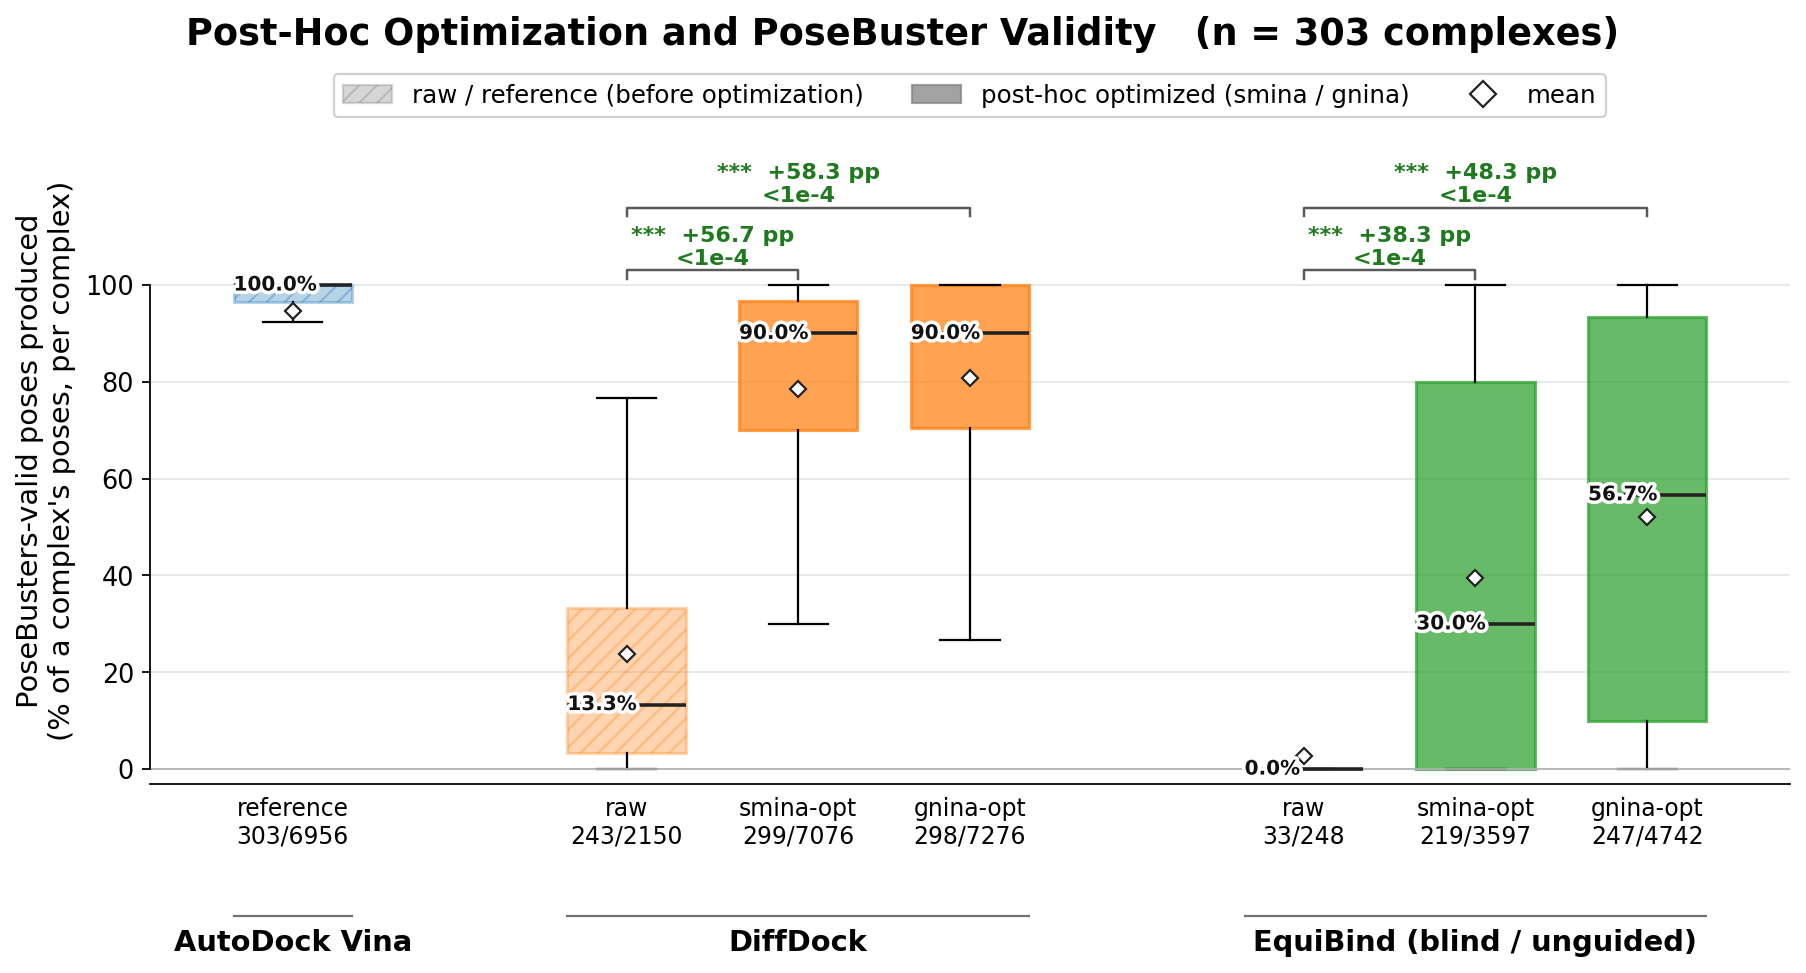
\includegraphics[width=\linewidth,height=0.78\textheight,keepaspectratio]{media/media/image2.png}
\caption{Post-hoc optimisation and PoseBusters validity}\label{fig:results-r1}
\end{figure}

Figure~\ref{fig:results-r1} shows per-complex PoseBusters-validity yield across the 303 benchmark complexes for raw and refined outputs. Post-hoc minimisation is the dominant driver of validity. The DiffDock median rises from 13.3\% to 90.0\%, and unguided EquiBind rises from 0\% to 56.7\% with gnina. The gains are near-unanimous across complexes and remain statistically detectable after Holm correction, with rank-biserial effects of 0.996 to 1.000 and adjusted p-values of approximately 4 \ensuremath{\times} 10\textsuperscript{-49} to 2 \ensuremath{\times} 10\textsuperscript{-3}. gnina is clearly stronger than smina for EquiBind, while the DiffDock refiners are much closer.

AutoDock Vina serves as the physics reference with a median per-complex yield of 100\%, a pooled validity of 94.8\% across all produced poses and at least one PoseBusters-valid pose for every one of the 303 complexes, that is full coverage with no ligand-preparation dropouts.

Because each tool returns a ranked list rather than a single pose, the depth of the pool a user inspects changes how many physically valid poses are available. Three pools, rank-1, best of top-15 and best of top-30, are compared in Table~\ref{tab:results-depth-recovery}. All depth gains reported in this chapter were assessed with exact two-sided McNemar tests on the discordant pairs, with Wilson score 95\% confidence intervals and Holm-Bonferroni correction within the depth family, a complex counting as recovered whenever any pose within the inspected pool is both PoseBusters-valid and within 2\angstrom{}.

In the pass-all analysis reported in Table~\ref{tab:results-depth-recovery}, deepening the inspected pool from rank-1 to top-15 adds 93 recovered complexes for AutoDock Vina (+30.7 percentage points), 63 for DiffDock (+20.8 points) and 16 for EquiBind (+5.3 points). These are the ranking-depth view of the same PoseBusters-valid, within-2\angstrom{} recovery tabulated across distance thresholds in Table~\ref{tab:results-near-native-form}, with which they agree at every reported depth.

\begin{longtable}[]{@{}
  >{\raggedright\arraybackslash}p{(\columnwidth - 10\tabcolsep) * \real{0.1756}}
  >{\raggedleft\arraybackslash}p{(\columnwidth - 10\tabcolsep) * \real{0.1385}}
  >{\raggedleft\arraybackslash}p{(\columnwidth - 10\tabcolsep) * \real{0.1573}}
  >{\raggedleft\arraybackslash}p{(\columnwidth - 10\tabcolsep) * \real{0.1573}}
  >{\raggedleft\arraybackslash}p{(\columnwidth - 10\tabcolsep) * \real{0.1859}}
  >{\raggedleft\arraybackslash}p{(\columnwidth - 10\tabcolsep) * \real{0.1853}}@{}}
\caption{PoseBusters Pass-All Recovery by Ranking Depth}\tabularnewline
\toprule\noalign{}
{\raggedright \textbf{Method}} & \centering\arraybackslash\textbf{Rank-1} & \centering\arraybackslash\textbf{Best of top-15} & \centering\arraybackslash\textbf{Best of top-30} & \centering\arraybackslash\textbf{top-1\ensuremath{\rightarrow}15 gain} & \centering\arraybackslash\textbf{top-15\ensuremath{\rightarrow}30 gain} \\
{\raggedright AutoDock Vina} & {\raggedright 55.5\% (168)} & {\raggedright 86.1\% (261)} & {\raggedright 88.5\% (268)} & {\raggedright +93 (+30.7\%) ***} & {\raggedright +7 (+2.3\%)} \\
\midrule\noalign{}
\endfirsthead
\caption[]{PoseBusters Pass-All Recovery by Ranking Depth (continued)}\tabularnewline
\toprule\noalign{}
{\raggedright \textbf{Method}} & \centering\arraybackslash\textbf{Rank-1} & \centering\arraybackslash\textbf{Best of top-15} & \centering\arraybackslash\textbf{Best of top-30} & \centering\arraybackslash\textbf{top-1\ensuremath{\rightarrow}15 gain} & \centering\arraybackslash\textbf{top-15\ensuremath{\rightarrow}30 gain} \\
{\raggedright AutoDock Vina} & {\raggedright 55.5\% (168)} & {\raggedright 86.1\% (261)} & {\raggedright 88.5\% (268)} & {\raggedright +93 (+30.7\%) ***} & {\raggedright +7 (+2.3\%)} \\
\midrule\noalign{}
\endhead
\bottomrule\noalign{}
\endlastfoot
DiffDock (smina) & 32.3\% (98) & 53.1\% (161) & 54.8\% (166) & +63 (+20.8\%) *** & +5 (+1.7\%) \\
EquiBind (gnina) & 15.2\% (46) & 20.5\% (62) & 20.8\% (63) & +16 (+5.3\%) *** & +1 (+0.3\%) \\
\multicolumn{6}{@{}l@{}}{%
two-sided McNemar tests with Holm-Bonferroni correction, *** p \textless{} 0.001, ** p \textless{} 0.01 and * p \textless{} 0.05} \\
\multicolumn{6}{@{}p{\dimexpr\columnwidth-6\tabcolsep\relax}@{}}{\footnotesize%
A complex is recovered when \emph{any} pose within the first $d$ ranked poses is both PoseBusters-valid and within 2\angstrom{}. This is the same PoseBusters-valid, within-2\angstrom{} recovery reported across distance thresholds in the near-nativeness and form analysis (Table~\ref{tab:results-near-native-form}), and the two coincide at every reported depth (168/261/268 for AutoDock Vina at rank-1/top-15/top-30).} \\
\end{longtable}
% RESOLVED 2026-07-26: Switched Table 5+6 to the existence gate (any pose in top-d that is PB-valid AND RMSD<=2A) = same definition as Table 7/19 (topk_recovery_validity.csv). Counts verified vs per_pose_metrics.csv: AutoDock 168/261/268, DiffDock-smina 98/161/166, EquiBind-gnina 46/62/63; Table 5 now equals Table 7's 2A placement column at depths 1/15/30. Table 6 recomputed as geometry-surfaced (+90/+63/+17 near-native gained; -0/-7/-2 remain PB-invalid) + validity-rescued (+3/+7/+1) = net +93/+63/+16.
\labelcurrenttable{tab:results-depth-recovery}

Almost all of these added complexes simply gain a near-native pose that was generated but under-ranked, so deeper pooling corrects mis-ranking rather than physical defects. PoseBusters validity has only a marginal net effect at this depth. It rescues a few complexes whose rank-1 near-native pose was invalid while excluding a few whose newly surfaced near-native pose still fails a check, so the valid recovery stays close to the raw near-native recovery.

\begin{longtable}[]{@{}
  >{\raggedright\arraybackslash}p{(\columnwidth - 6\tabcolsep) * \real{0.4286}}
  >{\raggedleft\arraybackslash}p{(\columnwidth - 6\tabcolsep) * \real{0.1716}}
  >{\raggedleft\arraybackslash}p{(\columnwidth - 6\tabcolsep) * \real{0.1859}}
  >{\raggedleft\arraybackslash}p{(\columnwidth - 6\tabcolsep) * \real{0.2139}}@{}}
\caption{Decomposition of the Rank-1 to Best-of-Top-15 Pass-All Gain}\tabularnewline
\toprule\noalign{}
{\raggedright \textbf{Contributions top-15 gain}} & \centering\arraybackslash\textbf{AutoDock Vina} & \centering\arraybackslash\textbf{DiffDock (smina)} & \centering\arraybackslash\textbf{EquiBind (gnina)} \\
\midrule\noalign{}
\endfirsthead
\caption[]{Decomposition of the Rank-1 to Best-of-Top-15 Pass-All Gain (continued)}\tabularnewline
\toprule\noalign{}
{\raggedright \textbf{Contributions top-15 gain}} & \centering\arraybackslash\textbf{AutoDock Vina} & \centering\arraybackslash\textbf{DiffDock (smina)} & \centering\arraybackslash\textbf{EquiBind (gnina)} \\
\midrule\noalign{}
\endhead
\bottomrule\noalign{}
\endlastfoot
Near-native poses gained\newline (RMSD \ensuremath{\leq} 2\angstrom{} gate) & +90 & +63 & +17 \\
of which remain PoseBusters-invalid & 0 & -7 & -2 \\
Valid near-native rescued from a\newline lower rank & +3 & +7 & +1 \\
Net valid complexes added & +93 *** & +63 *** & +16 *** \\
\multicolumn{4}{@{}l@{}}{%
Two-sided McNemar test with Holm-Bonferroni correction, where *** p \textless{} 0.001} \\
\end{longtable}
\labelcurrenttable{tab:results-depth-gain}

Deepening from rank-1 to the best of fifteen is highly significant for all three tools (p \textless{} 0.001), so a deeper pool taps a genuine reservoir of lower-ranked PoseBusters-valid poses, which for the deep-learning tools becomes accessible once gnina or smina minimisation has repaired their geometry.

\hypertarget{near-nativeness-and-form}{%
\subsection{Near-Nativeness and Form}\label{near-nativeness-and-form}}

Figures~\ref{fig:results-r2a} and \ref{fig:results-r2b} and Table~\ref{tab:results-near-native-form} summarise accuracy over the same 303 calibration complexes. The vertical axis reports the percentage of complexes for which a tool has at least one PoseBusters-valid pose within the distance threshold, evaluated over the best of its first d ranked poses.

Both figures are gated on PoseBusters validity and drawn at three ranking depths, with Figure~\ref{fig:results-r2a} measuring placement against as-placed crystal RMSD and Figure~\ref{fig:results-r2b} internal form against best-fit Kabsch RMSD.

Attention is drawn to the band between the top-1, top-15 and top-30 curves of each tool. Its width is the ranking headroom, that is the near-native valid poses that were generated but failed to rank first or within the top d, and it therefore separates sampling power from scoring power, a distinction the following paragraphs return to.

The three tools differ at every ranking depth on both metrics, with the Cochran\textquotesingle s Q omnibus tests significant throughout (placement p \textless{} 1e-22, form p \textless{} 1e-10). On placement at 2\angstrom{} the ordering is strict and every pairwise difference is significant under Holm-corrected exact McNemar tests, with AutoDock Vina ahead of DiffDock, which is in turn ahead of EquiBind, at rank-1 accuracies of 55.5\%, 32.3\% and 15.2\%. On form at 1\angstrom{} AutoDock Vina and DiffDock are statistically indistinguishable at rank-1 (McNemar p\_holm = 0.070), with Vina pulling significantly ahead once the pool deepens (p\_holm = 0.010 at top-15 and 0.016 at top-30), while both remain significantly ahead of EquiBind, at rank-1 accuracies of 55.1\%, 48.8\% and 30.7\%.

The deep-learning deficit is concentrated in placement rather than in conformational form, most sharply for EquiBind. Within each tool a Cochran's Q across the three depths confirms that ranking depth changes the outcome (Vina Q = 187, DiffDock Q = 127, EquiBind Q = 32, all p \textless{} 1e-6). The recovered share from top-1 to top-15 on placement, with Wilson 95\% intervals, is +30.7\% (25.8 to 36.1) for AutoDock Vina, +20.8\% (16.6 to 25.7) for DiffDock and only +5.3\% (3.3 to 8.4) for EquiBind. The further step from top-15 to top-30 adds at most 2.3\% for any tool, so almost all recoverable headroom is already present in a top-15 pool.

\begin{landscape}
\scriptsize
\setlength{\tabcolsep}{2pt}
\begin{longtable}[]{@{}
  >{\raggedright\arraybackslash}p{(\columnwidth - 26\tabcolsep) * \real{0.0870}}
  >{\raggedright\arraybackslash}p{(\columnwidth - 26\tabcolsep) * \real{0.1166}}
  >{\raggedright\arraybackslash}p{(\columnwidth - 26\tabcolsep) * \real{0.0673}}
  >{\raggedleft\arraybackslash}p{(\columnwidth - 26\tabcolsep) * \real{0.0080}}
  >{\raggedleft\arraybackslash}p{(\columnwidth - 26\tabcolsep) * \real{0.0649}}
  >{\raggedleft\arraybackslash}p{(\columnwidth - 26\tabcolsep) * \real{0.0729}}
  >{\raggedleft\arraybackslash}p{(\columnwidth - 26\tabcolsep) * \real{0.0729}}
  >{\raggedleft\arraybackslash}p{(\columnwidth - 26\tabcolsep) * \real{0.0729}}
  >{\raggedleft\arraybackslash}p{(\columnwidth - 26\tabcolsep) * \real{0.0729}}
  >{\raggedleft\arraybackslash}p{(\columnwidth - 26\tabcolsep) * \real{0.0729}}
  >{\raggedleft\arraybackslash}p{(\columnwidth - 26\tabcolsep) * \real{0.0729}}
  >{\raggedleft\arraybackslash}p{(\columnwidth - 26\tabcolsep) * \real{0.0729}}
  >{\raggedleft\arraybackslash}p{(\columnwidth - 26\tabcolsep) * \real{0.0729}}
  >{\raggedleft\arraybackslash}p{(\columnwidth - 26\tabcolsep) * \real{0.0729}}@{}}
\caption{Near-Nativeness and Form Recovery at Different Ranking Depths}\tabularnewline
\toprule\noalign{}
{} & {} & \multicolumn{2}{r}{%
{}} & \multicolumn{10}{>{\centering\arraybackslash}p{(\columnwidth - 26\tabcolsep) * \real{0.7210}}@{}}{%
Threshold (\angstrom{})} \\
\midrule\noalign{}
\endfirsthead
\caption[]{Near-Nativeness and Form Recovery at Different Ranking Depths (continued)}\tabularnewline
\toprule\noalign{}
{} & {} & \multicolumn{2}{r}{%
{}} & \multicolumn{10}{>{\centering\arraybackslash}p{(\columnwidth - 26\tabcolsep) * \real{0.7210}}@{}}{%
Threshold (\angstrom{})} \\
\midrule\noalign{}
\endhead
\bottomrule\noalign{}
\endlastfoot
Metric & \centering\arraybackslash Tool & \centering\arraybackslash Ranking Depth & \multicolumn{2}{>{\centering\arraybackslash}p{(\columnwidth - 26\tabcolsep) * \real{0.0729}}}{%
0.25} & \centering\arraybackslash 0.5 & \centering\arraybackslash 0.75 & \centering\arraybackslash 1 & \centering\arraybackslash 1.25 & \centering\arraybackslash 1.5 & \centering\arraybackslash 1.75 & \centering\arraybackslash 2 & \centering\arraybackslash 2.25 & \centering\arraybackslash 2.5 \\
\multirow{9}{*}{RMSD} & AutoDock & 1 & \multicolumn{2}{r}{%
0.7\%} & 9.9\% & 18.8\% & 31.7\% & 40.6\% & 47.2\% & 51.5\% & 55.5\% & 59.4\% & 62.7\% \\
& AutoDock & 15 & \multicolumn{2}{r}{%
1.0\%} & 14.9\% & 28.1\% & 49.5\% & 65.7\% & 75.9\% & 80.5\% & 86.1\% & 89.4\% & 91.8\% \\
& AutoDock & 30 & \multicolumn{2}{r}{%
1.0\%} & 14.9\% & 28.1\% & 49.5\% & 66.3\% & 77.9\% & 83.2\% & 88.5\% & 91.8\% & 93.4\% \\
& DiffDock + smina & 1 & \multicolumn{2}{r}{%
0.3\%} & 4.0\% & 10.9\% & 15.5\% & 21.1\% & 25.7\% & 30.0\% & 32.3\% & 33.7\% & 35.0\% \\
& DiffDock + smina & 15 & \multicolumn{2}{r}{%
1.0\%} & 9.6\% & 20.5\% & 29.7\% & 39.6\% & 45.2\% & 49.5\% & 53.1\% & 55.8\% & 57.1\% \\
& DiffDock + smina & 30 & \multicolumn{2}{r}{%
1.0\%} & 10.9\% & 21.8\% & 31.4\% & 40.6\% & 46.5\% & 51.5\% & 54.8\% & 57.8\% & 59.7\% \\
& EquiBind + gnina & 1 & \multicolumn{2}{r}{%
0.0\%} & 1.3\% & 2.0\% & 5.0\% & 9.2\% & 11.2\% & 13.5\% & 15.2\% & 16.2\% & 16.8\% \\
& EquiBind + gnina & 15 & \multicolumn{2}{r}{%
0.0\%} & 1.7\% & 4.0\% & 8.3\% & 12.5\% & 15.2\% & 17.8\% & 20.5\% & 21.8\% & 23.1\% \\
& EquiBind + gnina & 30 & \multicolumn{2}{r}{%
0.0\%} & 1.7\% & 4.3\% & 8.3\% & 12.5\% & 15.2\% & 17.8\% & 20.8\% & 22.1\% & 23.4\% \\
\multirow{9}{*}{Kabsch RMSD} & AutoDock & 1 & \multicolumn{2}{r}{%
11.6\%} & 28.1\% & 41.9\% & 55.1\% & 68.0\% & 72.3\% & 77.6\% & 81.5\% & 85.8\% & 87.8\% \\
& AutoDock & 15 & \multicolumn{2}{r}{%
19.1\%} & 37.0\% & 58.4\% & 77.2\% & 88.1\% & 92.1\% & 95.7\% & 97.0\% & 97.7\% & 98.4\% \\
& AutoDock & 30 & \multicolumn{2}{r}{%
19.8\%} & 38.9\% & 60.4\% & 79.5\% & 89.4\% & 93.7\% & 97.0\% & 98.0\% & 98.7\% & 98.7\% \\
& DiffDock + smina & 1 & \multicolumn{2}{r}{%
11.2\%} & 23.4\% & 36.0\% & 48.8\% & 57.8\% & 63.7\% & 69.6\% & 75.2\% & 77.9\% & 79.5\% \\
& DiffDock + smina & 15 & \multicolumn{2}{r}{%
19.8\%} & 37.6\% & 55.8\% & 70.0\% & 76.6\% & 84.5\% & 90.8\% & 93.4\% & 93.7\% & 94.4\% \\
& DiffDock + smina & 30 & \multicolumn{2}{r}{%
21.5\%} & 41.9\% & 59.7\% & 73.3\% & 81.9\% & 91.4\% & 95.1\% & 96.4\% & 97.0\% & 97.7\% \\
& EquiBind + gnina & 1 & \multicolumn{2}{r}{%
5.3\%} & 11.2\% & 18.5\% & 30.7\% & 38.3\% & 48.2\% & 53.1\% & 60.7\% & 64.0\% & 68.0\% \\
& EquiBind + gnina & 15 & \multicolumn{2}{r}{%
13.5\%} & 27.4\% & 37.3\% & 46.5\% & 56.8\% & 66.7\% & 69.3\% & 74.9\% & 75.9\% & 77.9\% \\
& EquiBind + gnina & 30 & \multicolumn{2}{r}{%
15.2\%} & 30.0\% & 39.3\% & 50.2\% & 58.8\% & 68.3\% & 71.0\% & 75.2\% & 76.6\% & 78.2\% \\
\end{longtable}
\labelcurrenttable{tab:results-near-native-form}
\end{landscape}

The band between the curves quantifies that separation \cite{ref003,ref004,ref005}, since it shows how often a good pose is generated but not ranked first.

AutoDock Vina leads on both placement and form at the reported depths, but its ranking headroom is still substantial. Rank-1 valid-near-native recovery of 55.5\% rises to 86.1\% when the best of the top-15 poses is selected retrospectively. The stronger conclusion is therefore that Vina ranks better than the tested alternatives while still leaving a meaningful selection gap, consistent with the longstanding distinction between sampling and scoring \cite{ref003}, \cite{ref050}, \cite{ref052}.

DiffDock\textquotesingle s rank-1 pose is near-native in 32.3\% and form-correct in 48.8\% of the calibration set. Its top-30 pool contains a valid near-native pose for 54.8\% of complexes on placement and a form-correct pose for 73.3\% at the primary 1 \angstrom{} Kabsch threshold. Although DiffDock provides a confidence model \cite{ref024}, independent evaluations likewise show that generative docking can sample acceptable poses more reliably than it ranks them \cite{ref013}, \cite{ref032}, \cite{ref035}.

\begin{figure}[!htbp]
\centering
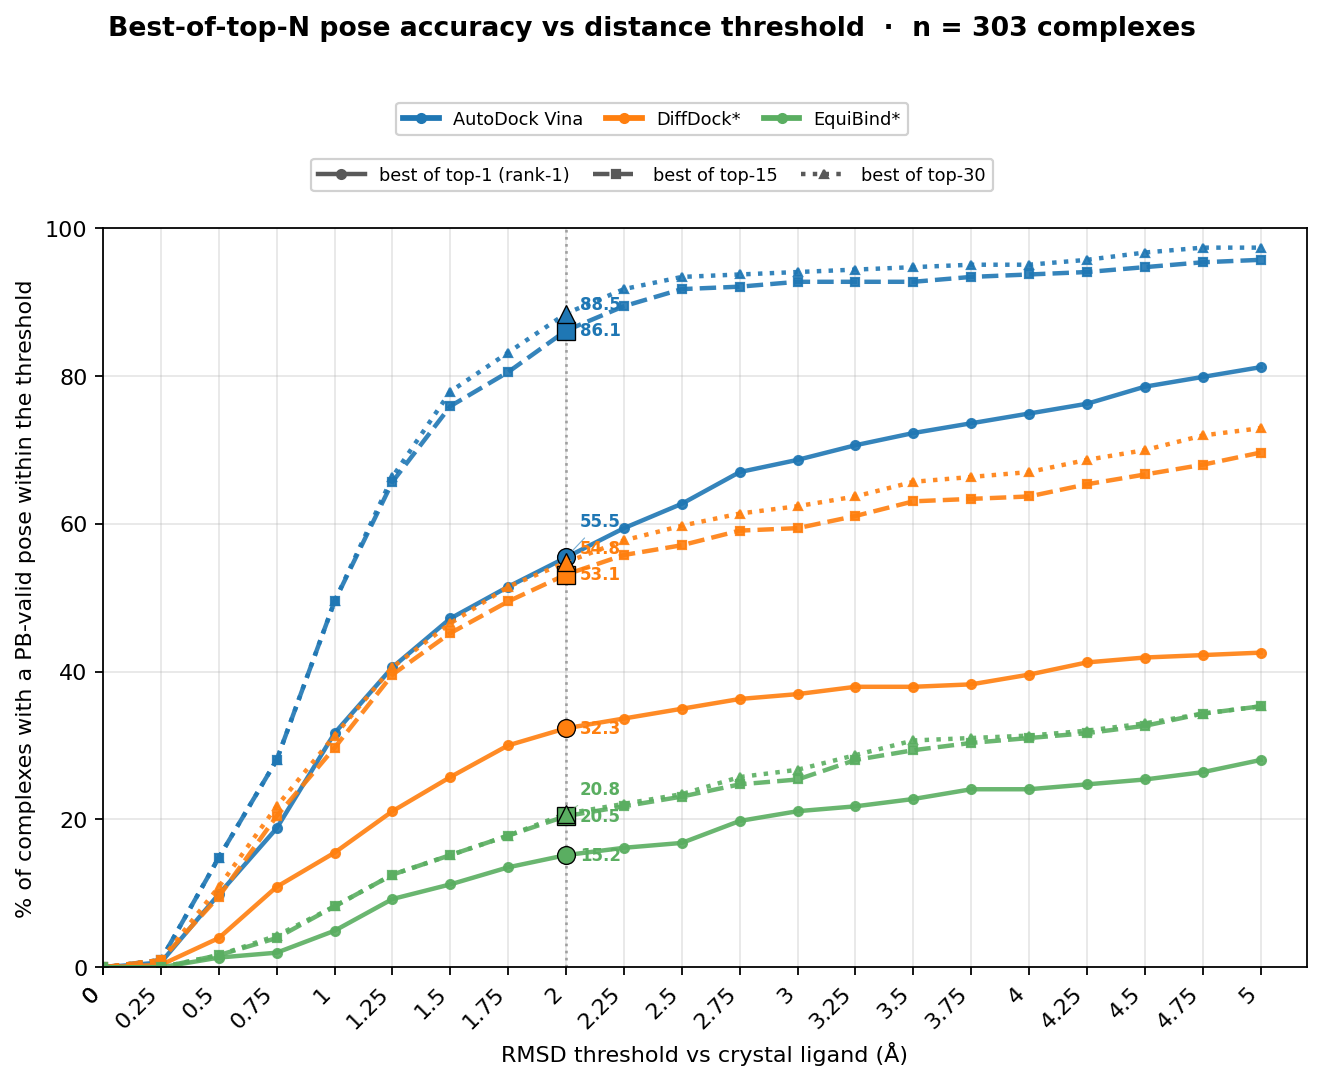
\includegraphics[width=\linewidth,height=0.78\textheight,keepaspectratio]{media/media/image3.png}
\caption{Best-of-top-N accuracy against the as-placed crystal RMSD}\label{fig:results-r2a}
\end{figure}

EquiBind's ranking depth improvement on near-nativeness is limited to +5.3\% from rank-1 to top-15. The single-shot regression model barely samples distinct alternatives, so on placement it is sampling-bound rather than ranking-bound and no rescorer can recover poses that were never generated. This is a genuinely different failure mode from DiffDock\textquotesingle s, one that RMSD-only leaderboards conflate and that only the ranking-depth axis exposes.

Kabsch RMSD separates internal conformation from placement. At the primary 1 \angstrom{} threshold and the best-of-top-30 depth, form recovery is 79.5\% for AutoDock Vina and 73.3\% for DiffDock. At the more permissive 2 \angstrom{} threshold, the corresponding values are 98.0\% and 96.4\%. Both tools therefore score substantially higher on form than on in-place placement. For DiffDock, this pattern indicates that conformer generation is stronger than site placement and ranking, consistent with its generative treatment of torsional, rotational and translational degrees of freedom \cite{ref024}.

EquiBind remains the weakest on form, reaching 30.7\% at rank-1 and 50.2\% at best-of-top-30 under the primary 1 \angstrom{} threshold. This points to internal-geometry error in addition to misplacement and is consistent with current evaluations in which direct regression models trail diffusion and hybrid methods on combined geometry and physical validity \cite{ref013}, \cite{ref035}. Its 19.5 percentage-point depth gain shows that the conformer-expanded pipeline sometimes contains an acceptable shape, even when that shape is not placed correctly.

Because the near-native valid poses already exist in a shallow top-15 pool, the highest-leverage intervention for DiffDock is a better pose selector rather than more sampling, which is the direction the field has converged on \cite{ref006,ref011}. For EquiBind on placement the same logic does not apply, since no rescorer can recover poses that were never sampled.

\begin{figure}[!htbp]
\centering

\includegraphics[width=\linewidth,height=0.78\textheight,keepaspectratio]{media/media/image4.png}
\caption{The same best-of-top-N accuracy against the best-fit (Kabsch) RMSD threshold}\label{fig:results-r2b}
\end{figure}

The depth-resolved curves separate generation from selection. AutoDock Vina leads at every depth but retains material ranking headroom. DiffDock is chiefly selection-limited because valid near-native poses often appear below rank-1, and EquiBind is chiefly sampling- and placement-limited because its best-of-pool recovery remains low \cite{ref003}, \cite{ref013}, \cite{ref024}, \cite{ref035}. A top-15 pool captures almost all observed headroom, with at most 2.3 additional percentage points from extending the pool to 30.

Figure~\ref{fig:results-r3} separates the two ways a valid pose can be wrong, plotting in-place RMSD against best-fit Kabsch RMSD so that placement-limited poses (correctly shaped but mislocated), form-limited poses (placed roughly right but folded wrong) and mixed cases fall in distinct regions, with the three columns widening the accepted pool from rank-1 to the best of the top-5 and top-15 and the arrow tracing each cohort median\textquotesingle s drift from rank-1. Table~\ref{tab:results-placement-form} gives the underlying distributions.\footnote{Poses whose docked centroid lies more than 8\angstrom{} from the crystal-ligand site are treated as off-receptor and excluded before plotting, which removes 3,175 poses at the top-15 depth and leaves 7,400 on-receptor PoseBusters-valid poses. Both axes are then clipped at 5\angstrom{} to keep the dense near-native core legible, so a further 2,824 of those 7,400 poses lie beyond the frame and are not drawn. This is consistent with the in-place third quartiles above 5\angstrom{} reported for AutoDock Vina and EquiBind in Table~\ref{tab:results-placement-form}.}

\begin{figure}[!htbp]
\centering

\includegraphics[width=\linewidth,height=0.78\textheight,keepaspectratio]{media/media/image5.png}
\caption{Form versus placement across ranking depth}\label{fig:results-r3}
\end{figure}

AutoDock Vina has a valid pose for almost every complex. Yet increasing ranking depth causes a decline in placement accuracy. Its median in-place RMSD drifts from 1.5\angstrom{} at rank-1 to 4.6\angstrom{} at top-15, the largest movement of any tool (+3.18\angstrom{}, Friedman p \ensuremath{\approx} 4e-40), while its placement-limited share swells from 46\% to 76\% and its form-limited share shrinks from 28\% to 9\%. Increasing ranking depth mostly adds correctly-shaped ligands scattered in the wrong place, consistent with the highest pose diversity of the three at a 6.2\angstrom{} within-complex spread, so its ranking is informative only near the very top.

DiffDock is the depth-stable tool. Its rank-1 coverage is lower, but its cloud barely moves, with an in-place drift of only +0.32\angstrom{} and a form error that is statistically depth-invariant (Friedman p = 0.059). Widening the pool fifteen-fold leaves the median near 1.5 to 1.7\angstrom{} in placement and about 0.9\angstrom{} in form, and by top-5 and top-15 it is significantly the best tool on both axes. Part of that flatness is low pose diversity, namely a 2.2\angstrom{} spread of near-duplicate poses, so its robustness to depth is partly a reluctance to diversity.

EquiBind can generate PoseBusters-valid output, but validity does not translate into reliable placement. At least one valid pose occurs somewhere in the full output for 247 of 303 complexes, yet valid-near-native recovery remains only 20.5\% by the top-15 depth. Its rank-1 median in-place RMSD of 2.9 \angstrom{} already exceeds the 2 \angstrom{} near-native threshold. gnina refinement can remove some local geometric defects, but it does not correct the pipeline\textquotesingle s gross placement failures.

Deeper ranks therefore add valid but mislocated poses for every tool, steeply for AutoDock and EquiBind and barely for DiffDock, so placement rather than internal form is the axis that degrades with depth. DiffDock\textquotesingle s more form-limited colouring is an artefact of its near-solved placement inflating the form-to-placement ratio, since its absolute form RMSD is the lowest of the three.

\begin{landscape}
\scriptsize
\setlength{\tabcolsep}{2pt}
\begin{longtable}[]{@{}
  >{\raggedright\arraybackslash}p{(\columnwidth - 26\tabcolsep) * \real{0.1319}}
  >{\raggedleft\arraybackslash}p{(\columnwidth - 26\tabcolsep) * \real{0.0736}}
  >{\raggedleft\arraybackslash}p{(\columnwidth - 26\tabcolsep) * \real{0.0589}}
  >{\raggedleft\arraybackslash}p{(\columnwidth - 26\tabcolsep) * \real{0.0668}}
  >{\raggedleft\arraybackslash}p{(\columnwidth - 26\tabcolsep) * \real{0.0668}}
  >{\raggedleft\arraybackslash}p{(\columnwidth - 26\tabcolsep) * \real{0.0668}}
  >{\raggedleft\arraybackslash}p{(\columnwidth - 26\tabcolsep) * \real{0.0670}}
  >{\raggedleft\arraybackslash}p{(\columnwidth - 26\tabcolsep) * \real{0.0668}}
  >{\raggedleft\arraybackslash}p{(\columnwidth - 26\tabcolsep) * \real{0.0668}}
  >{\raggedleft\arraybackslash}p{(\columnwidth - 26\tabcolsep) * \real{0.0668}}
  >{\raggedleft\arraybackslash}p{(\columnwidth - 26\tabcolsep) * \real{0.0670}}
  >{\raggedleft\arraybackslash}p{(\columnwidth - 26\tabcolsep) * \real{0.0668}}
  >{\raggedleft\arraybackslash}p{(\columnwidth - 26\tabcolsep) * \real{0.0668}}
  >{\raggedleft\arraybackslash}p{(\columnwidth - 26\tabcolsep) * \real{0.0670}}@{}}
\caption{Placement-versus-Form Distributions by Tool and Ranking Depth}\tabularnewline
\toprule\noalign{}
\shortstack[l]{\textbf{Tool}\\\textbf{(Ranking Depth)}\strut} & \centering\arraybackslash\textbf{n poses} & \centering\arraybackslash\textbf{Valid complexes} & \centering\arraybackslash\textbf{Coverage\%} & \centering\arraybackslash\textbf{In-place median (\angstrom{})} & \centering\arraybackslash\textbf{In-place Q1} & \centering\arraybackslash\textbf{In-place Q3} & \centering\arraybackslash\textbf{Form median (\angstrom{})} & \centering\arraybackslash\textbf{Form Q1} & \centering\arraybackslash\textbf{Form Q3} & \centering\arraybackslash\textbf{Median r} & \centering\arraybackslash\textbf{\% place-lim} & \centering\arraybackslash\textbf{\% mixed} & \centering\arraybackslash\textbf{\% form-lim} \\
\midrule\noalign{}
\endfirsthead
\caption[]{Placement-versus-Form Distributions by Tool and Ranking Depth (continued)}\tabularnewline
\toprule\noalign{}
\shortstack[l]{\textbf{Tool}\\\textbf{(Ranking Depth)}\strut} & \centering\arraybackslash\textbf{n poses} & \centering\arraybackslash\textbf{Valid complexes} & \centering\arraybackslash\textbf{Coverage\%} & \centering\arraybackslash\textbf{In-place median (\angstrom{})} & \centering\arraybackslash\textbf{In-place Q1} & \centering\arraybackslash\textbf{In-place Q3} & \centering\arraybackslash\textbf{Form median (\angstrom{})} & \centering\arraybackslash\textbf{Form Q1} & \centering\arraybackslash\textbf{Form Q3} & \centering\arraybackslash\textbf{Median r} & \centering\arraybackslash\textbf{\% place-lim} & \centering\arraybackslash\textbf{\% mixed} & \centering\arraybackslash\textbf{\% form-lim} \\
\midrule\noalign{}
\endhead
\bottomrule\noalign{}
\endlastfoot
AutoDock (1) & 288 & 288 & 95\% & 1.473 & 0.75 & 3.263 & 0.871 & 0.406 & 1.45 & 0.38 & 46.2\% & 25.3\% & 28.5\% \\
AutoDock (5) & 1412 & 300 & 99\% & 3.319 & 1.611 & 5.656 & 1.162 & 0.665 & 1.838 & 0.18 & 62.4\% & 19.3\% & 18.3\% \\
AutoDock (15) & 3920 & 301 & 99.3\% & 4.649 & 2.797 & 6.554 & 1.328 & 0.799 & 2.071 & 0.095 & 76.2\% & 14.4\% & 9.3\% \\
DiffDock (1) & 148 & 148 & 48.8\% & 1.372 & 0.734 & 2.93 & 0.856 & 0.471 & 1.384 & 0.464 & 39.2\% & 30.4\% & 30.4\% \\
DiffDock (5) & 718 & 214 & 70.6\% & 1.478 & 0.779 & 3.75 & 0.857 & 0.498 & 1.451 & 0.443 & 41.4\% & 34.0\% & 24.7\% \\
DiffDock (15) & 1953 & 241 & 79.5\% & 1.694 & 0.856 & 4.658 & 0.913 & 0.516 & 1.568 & 0.385 & 45.4\% & 32.3\% & 22.3\% \\
EquiBind (1) & 126 & 126 & 41.6\% & 2.933 & 1.342 & 5.885 & 1.128 & 0.744 & 1.909 & 0.172 & 61.9\% & 20.6\% & 17.5\% \\
EquiBind (5) & 588 & 142 & 46.9\% & 3.672 & 1.989 & 6.307 & 1.244 & 0.762 & 1.979 & 0.137 & 71.1\% & 17.3\% & 11.6\% \\
EquiBind (15) & 1527 & 147 & 48.5\% & 4.138 & 2.559 & 6.574 & 1.291 & 0.782 & 2.019 & 0.106 & 76.7\% & 15.3\% & 8.0\% \\
\end{longtable}
\labelcurrenttable{tab:results-placement-form}
\end{landscape}

\hypertarget{cross-tool-clustering}{%
\subsection{Cross-Tool Clustering}\label{cross-tool-clustering}}

Accuracy and validity describe each tool separately, whereas clustering tests agreement about binding regions. For every complex, poses from all three tools were pooled without prefiltering on PoseBusters validity and clustered by ligand centroid. The cluster centre nearest the crystal ligand was treated as the recovered crystallographic region. Figure~\ref{fig:results-r4} reports recovery within the top-N ranked poses for individual tools and combinations, with the corresponding rates in Table~\ref{tab:results-cluster-recovery}.

\begin{figure}[!htbp]
\centering

\includegraphics[width=\linewidth,height=0.78\textheight,keepaspectratio]{media/media/image6.png}
\caption{Top-N crystal-cluster co-recovery. Each lower-triangular panel is one ranking depth}\label{fig:results-r4}
\end{figure}

AutoDock Vina reaches the true pocket for 95\% of complexes at rank 1 and outperforms DiffDock (56\%) and EquiBind (40\%) by a wide margin. This placement gap reflects the configured workflows rather than the method classes. AutoDock Vina searched a crystal-ligand-centred box that already localised the correct pocket, whereas DiffDock and EquiBind received no binding-site information and searched blind, so the comparison is least equal on precisely the quantity measured here, namely pocket localisation. While DiffDock's poses reach the crystal cluster with increasing rank (+27\% rank 1 to 15), EquiBind is near flat (+8\% rank 1 to 15). The two learned tools are redundant rather than complementary, reaching or missing the same complexes at every depth (\ensuremath{\phi} falling from +0.46 to +0.22, Fisher p \ensuremath{\leq} 1e-4), so stacking EquiBind on DiffDock adds little coverage.

\begin{longtable}[]{@{}
  >{\raggedright\arraybackslash}p{(\columnwidth - 8\tabcolsep) * \real{0.3570}}
  >{\centering\arraybackslash}p{(\columnwidth - 8\tabcolsep) * \real{0.1607}}
  >{\centering\arraybackslash}p{(\columnwidth - 8\tabcolsep) * \real{0.1607}}
  >{\centering\arraybackslash}p{(\columnwidth - 8\tabcolsep) * \real{0.1607}}
  >{\centering\arraybackslash}p{(\columnwidth - 8\tabcolsep) * \real{0.1608}}@{}}
\caption{Crystal-Cluster Reach and Co-Reach by Ranking Depth}\tabularnewline
\toprule\noalign{}
{\raggedright \textbf{Statistic}} & \centering\arraybackslash\textbf{top-1} & \centering\arraybackslash\textbf{top-5} & \centering\arraybackslash\textbf{top-10} & \centering\arraybackslash\textbf{top-15} \\
\midrule\noalign{}
\endfirsthead
\caption[]{Crystal-Cluster Reach and Co-Reach by Ranking Depth (continued)}\tabularnewline
\toprule\noalign{}
{\raggedright \textbf{Statistic}} & \centering\arraybackslash\textbf{top-1} & \centering\arraybackslash\textbf{top-5} & \centering\arraybackslash\textbf{top-10} & \centering\arraybackslash\textbf{top-15} \\
\midrule\noalign{}
\endhead
\bottomrule\noalign{}
\endlastfoot
AutoDock Vina reach {[}95\% CI{]} & 95 {[}92--97{]} & 98 {[}95--99{]} & 98 {[}95--99{]} & 98 {[}96--99{]} \\
DiffDock reach {[}95\% CI{]} & 56 {[}51--62{]} & 77 {[}72--82{]} & 81 {[}76--85{]} & 83 {[}79--87{]} \\
EquiBind reach {[}95\% CI{]} & 40 {[}35--46{]} & 46 {[}40--52{]} & 48 {[}42--53{]} & 48 {[}43--54{]} \\
DiffDock + EquiBind co-reach \ensuremath{\phi}\footnote{The AutoDock pairs cannot be tested at its reach ceiling, and three-way agreement exceeds chance at every depth (96 against 65 expected complexes at top-1, rising to 132 against 119 at top-15, permutation p \ensuremath{\leq} 2.0e-4), which is the DiffDock and EquiBind coupling carried through a near-constant AutoDock.} & +0.46 & +0.29 & +0.24 & +0.22 \\
AutoDock pairs co-reach \ensuremath{\phi} & n/e & n/e & n/e & n/e \\
All three reach, observed / expected & 96 / 65 & 123 / 105 & 128 / 114 & 132 / 119 \\
\end{longtable}
\labelcurrenttable{tab:results-cluster-recovery}

\begin{figure}[!htbp]
\centering
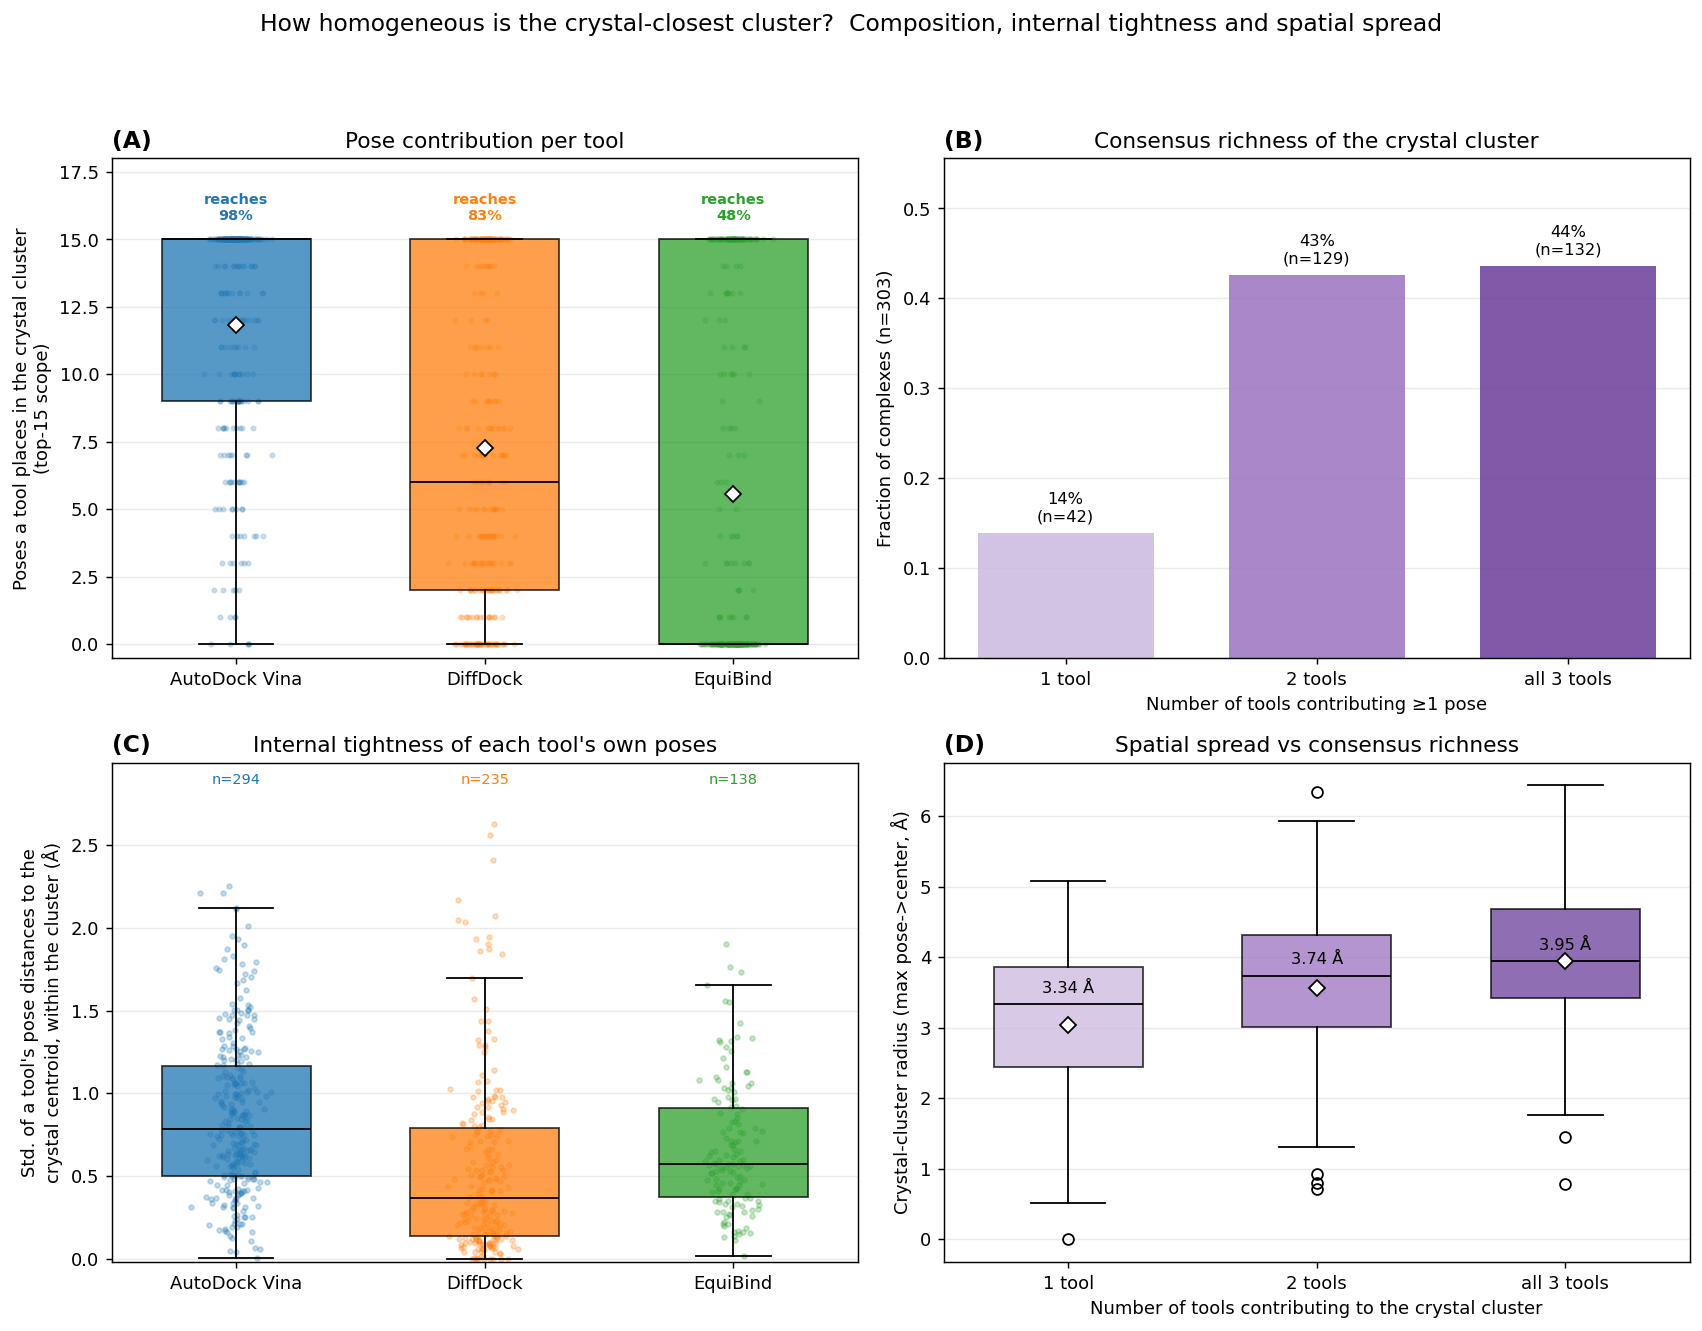
\includegraphics[width=\linewidth,height=0.78\textheight,keepaspectratio]{media/media/image7.png}
\caption{Composition and geometry of the crystal-closest cluster}\label{fig:results-r5}
\end{figure}

Figure~\ref{fig:results-r5} (A) shows AutoDock floods the pocket with a median of fifteen in-cluster poses out of fifteen ranked (98.3\% reach), DiffDock is moderate (83.2\% reach, median six poses) and EquiBind is all-or-nothing (48.2\% reach, median zero), a strict ordering on both pose count (Friedman \ensuremath{\chi}\textsuperscript{2} = 140.1, Kendall W = 0.231) and reach (Cochran's Q = 213.2, all pairs significant). As evident in Figure~\ref{fig:results-r5} (B) The correct pocket is usually a multi-tool basin, yet the consensus is polarised, namely complexes tend to be solved either by exactly one tool (42 against 28.5 expected, usually AutoDock alone) or by all three (132 against 119.4 expected, permutation p = 2.0e-4), with exactly two contributing tools under-represented (129 against 154.6 expected). Internal tightness in Figure~\ref{fig:results-r5} (C) inverts the reach order, surprisingly DiffDock's own poses being tightest at a median 0.37\angstrom{}. In contrast, AutoDock's poses are the loosest at 0.78\angstrom{} (Kruskal--Wallis H = 80.5, p \textless{} 1e-4, \ensuremath{\varepsilon}\textsuperscript{2} = 0.118).

Cluster radius rises from a median 3.34 \angstrom{} to 3.95 \angstrom{} as more tools contribute poses, but the trend disappears after controlling for pose count (partial \ensuremath{\rho} = \ensuremath{-}0.03, p = 0.56). The partition is reproducible under resampling (median bootstrap Jaccard 0.76). Internal indices are interpreted only for eligible multi-cluster complexes. Under the separate 4 \angstrom{} crystal-site threshold, the retrospective oracle finds a recovered cluster in 99\% of complexes, whereas the best inexpensive first-cluster rule reaches 86.5\%. This gap is a site-ranking problem. The crystal-compatible region is often represented somewhere in the rank-15 ensemble, but selecting it prospectively remains difficult.

In this benchmark, binding-site agreement is driven by AutoDock and DiffDock with EquiBind as the consensus bottleneck. The only real redundancy is between the two learned tools. The clustering is geometrically sound and the crystal pocket is almost always present, i.e. the residual loss is in ranking and not search. Pooling buys breadth at the cost of proximity, the three-tool ensemble reaching 99\% of pockets but with a worse median oracle distance of 1.23\angstrom{} than AutoDock at 0.39\angstrom{} alone.

\begin{figure}[!htbp]
\centering

\includegraphics[width=\linewidth,height=0.78\textheight,keepaspectratio]{media/media/image8.png}
\caption{Cluster-quality assessment (n = 303, 8 \angstrom{} centroid-clustering cut and 4 \angstrom{} crystal-site recovery threshold). Panels A-C show internal-validity indices, panel D compactness against separation, panel E bootstrap stability and panel F precision-at-one of five ranking rules against the oracle ceiling}\label{fig:results-r6}
\end{figure}

\hypertarget{interaction-and-contact-analysis}{%
\subsection{Interaction and Contact Analysis}\label{interaction-and-contact-analysis}}

The purpose of docking is to reproduce the protein--ligand interactions that drive binding. The interactions of the crystal ligand poses are compared with the interactions of PoseBusterss-valid poses produced by the toolchains. Figure~\ref{fig:results-r7} reports the mean Jaccard overlap between typed interaction fingerprints, where each tool\textquotesingle s repertoire for a complex is the union of its top-5 ranked poses and the overlap is averaged over all shared complexes.

\begin{figure}[!htbp]
\centering

\includegraphics[width=\linewidth,height=0.78\textheight,keepaspectratio]{media/media/image9.png}
\caption{Mean Jaccard similarity of interaction fingerprints}\label{fig:results-r7}
\end{figure}

AutoDock Vina has the highest mean typed-interaction Jaccard similarity to the crystal fingerprint (0.67), followed by DiffDock (0.44) and EquiBind (0.37). Pairwise tool similarities are lower, at 0.36 to 0.43, showing that the methods often make different contact hypotheses. Because Jaccard combines shared and non-shared interactions, these values should not be interpreted as contact recall. They show overall fingerprint agreement, not the fraction of native interactions recovered.

Figure~\ref{fig:results-r8} resolves precision, recall and F1 against pose rank k, where k = 1 is each tool\textquotesingle s own top-ranked PoseBusters-valid pose.

\begin{figure}[!htbp]
\centering
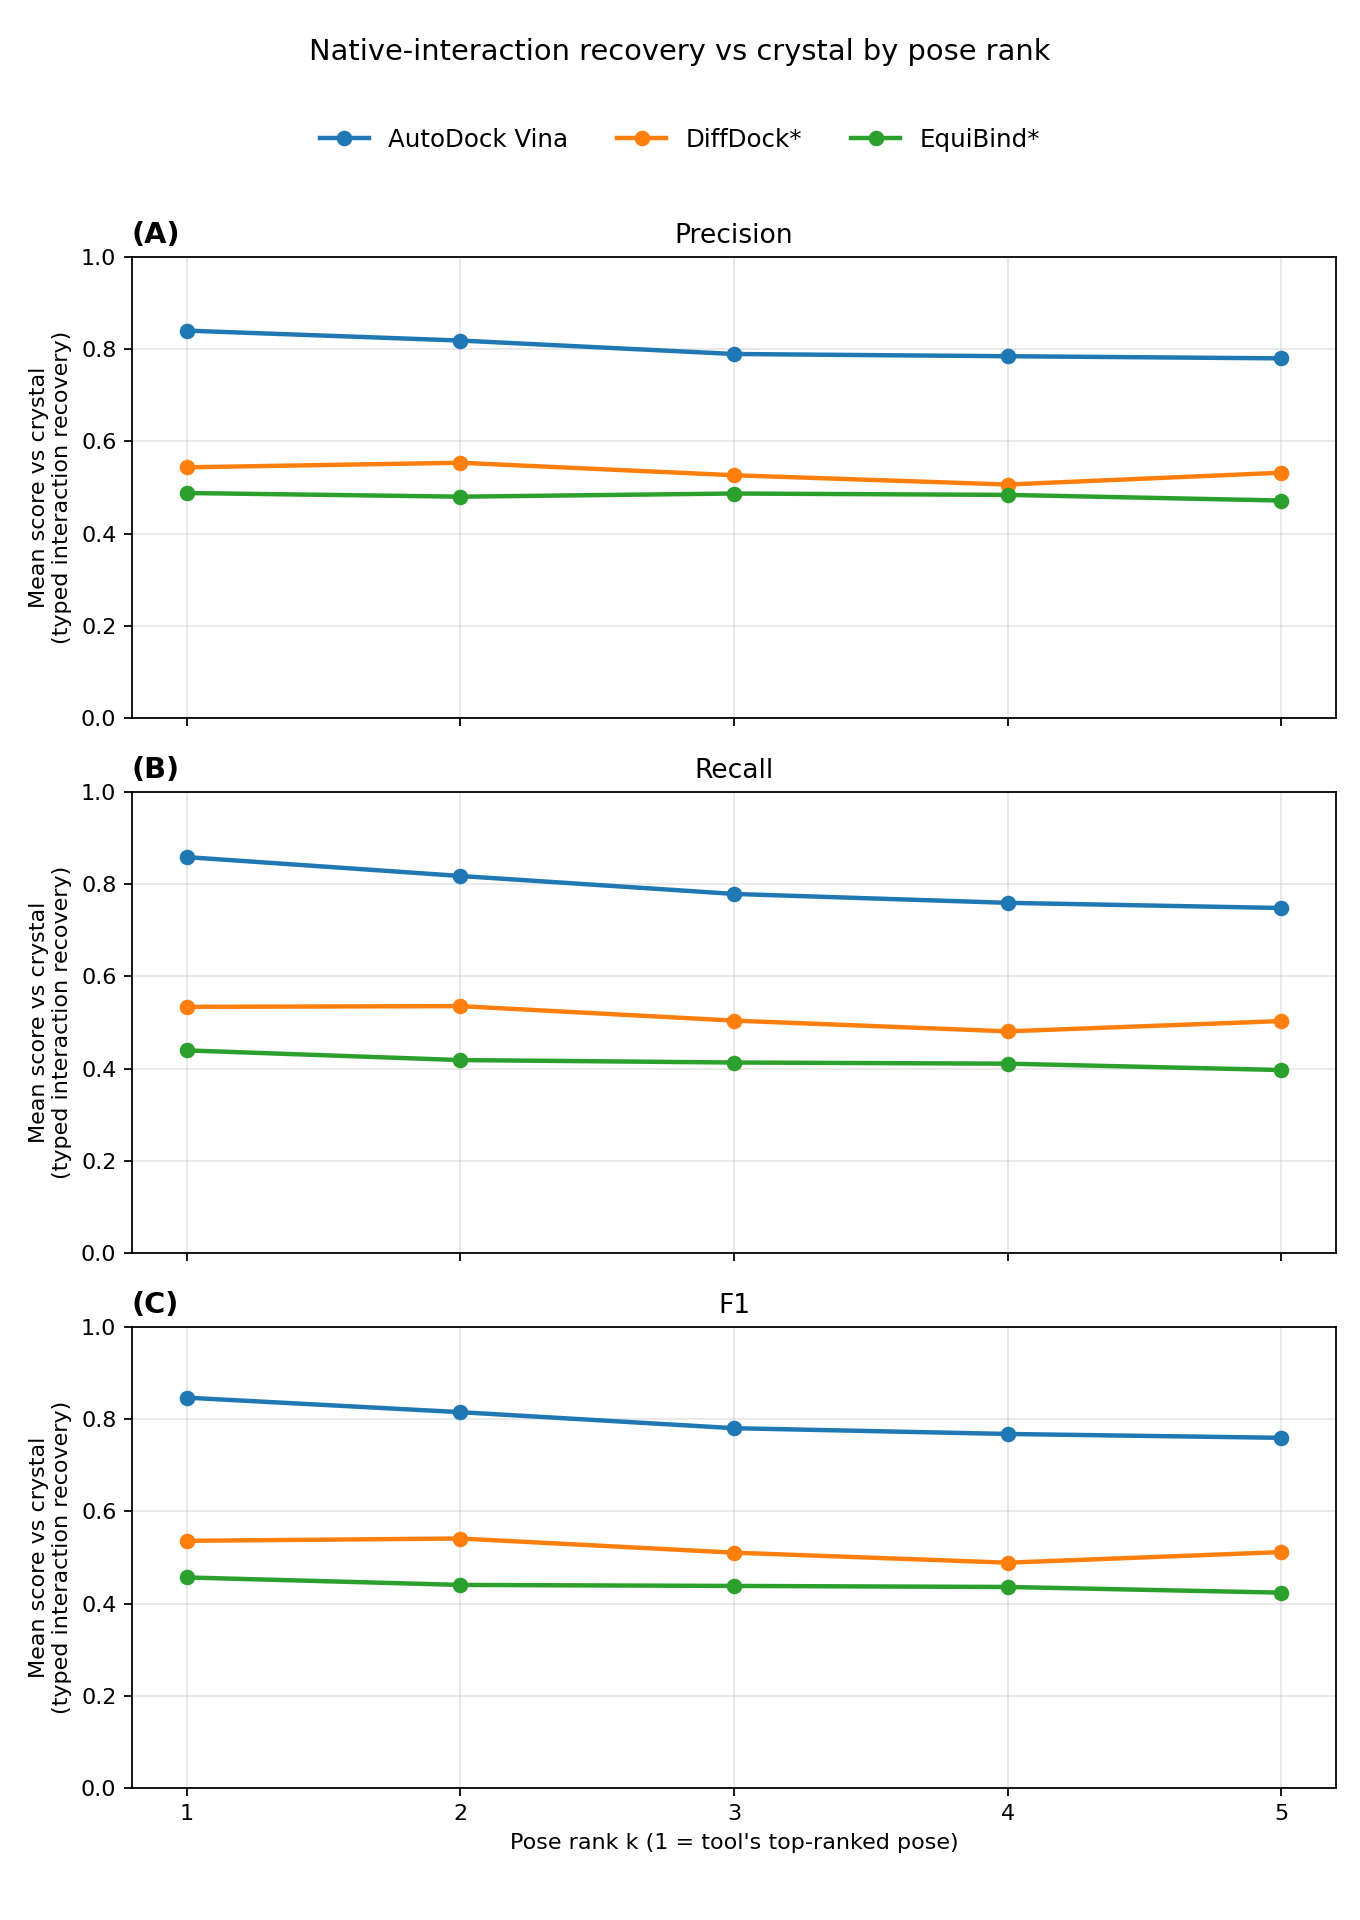
\includegraphics[width=\linewidth,height=0.78\textheight,keepaspectratio]{media/media/image10.png}
\caption{Native-interaction recovery versus the crystal by pose rank (1--5)}\label{fig:results-r8}
\end{figure}

AutoDock recovers native interactions far more completely, easing from an F1 of about 0.85 at rank 1 to 0.76 at rank 5, against roughly 0.54 to 0.51 for DiffDock and 0.46 to 0.42 for EquiBind. A per-complex Kendall \ensuremath{\tau} between rank and score, tested with a one-sample Wilcoxon signed-rank against zero and BH-corrected across the nine tool-by-metric cells, confirms that AutoDock\textquotesingle s own ranking puts better poses first (\ensuremath{\tau} = \ensuremath{-}0.32, \ensuremath{-}0.36 and \ensuremath{-}0.40 for precision, recall and F1, all p \textless{} 0.001, large effect). EquiBind\textquotesingle s gnina-affinity rank works for recall and F1 (\ensuremath{\tau} = \ensuremath{-}0.29 and \ensuremath{-}0.20, both significant) and only marginally for precision. DiffDock\textquotesingle s native confidence is uninformative for interaction recovery (\ensuremath{\tau} \ensuremath{\approx} 0 on all three, none significant), so its rank-1 pose recovers no more native contacts than its rank-5.

Figure~\ref{fig:results-r9} decomposes each pose\textquotesingle s typed contacts into matched native contacts recovered, missed native contacts absent, and spurious non-native contacts invented.

\begin{figure}[!htbp]
\centering

\includegraphics[width=\linewidth,height=0.78\textheight,keepaspectratio]{media/media/image11.png}
\caption{Matched, missed and spurious typed contacts versus the crystal, by pose rank}\label{fig:results-r9}
\end{figure}

AutoDock is matched-dominated, recovering about 31 native contacts against only 5 missed at rank 1 and 27 against 9 by rank 5, with few spurious contacts (about 6 to 8). EquiBind is the mirror image, missing more native contacts than it recovers at every rank, near 15 matched against 19 to 21 missed, so it systematically under-reproduces the native network. DiffDock is balanced, near 19 matched against 16 to 17 missed and crossing only at rank 4, but carries the most spurious contacts at 13 to 14 per pose, so it invents the most non-native chemistry. The same rank test orders AutoDock cleanly across all three classes (\ensuremath{\tau} = \ensuremath{-}0.36 matched, +0.36 missed, +0.32 spurious, all significant) and EquiBind on matched and missed (\ensuremath{\pm}0.29), whereas DiffDock\textquotesingle s counts are flat.

Taken together, AutoDock Vina reproduces the native interaction pattern most faithfully and its confidence ranking already surfaces close to its best pose, DiffDock\textquotesingle s contacts are moderately faithful but under-ranked so a re-scorer stands to help it most, and EquiBind is limited at source, recovering few native contacts regardless of rank.

\protect\hypertarget{_Toc235735934}{}{}

\hypertarget{experimental-dataset-1}{%
\section{Experimental Dataset}\label{experimental-dataset-1}}

The experimental evaluation asks whether the tool ordering established against crystallographic references survives on a target of genuine pharmacological interest, and whether the large benchmark library can stand in for the compounds that actually matter. That target is the human Orai1 channel, docked with the three functionally validated modulators 2-APB, GSK-7975A and Synta-66, and it removes the benchmark\textquotesingle s most valuable asset, since no ligand-bound Orai structure exists and the receptor is an ensemble of molecular-dynamics snapshots rather than a crystal. Every accuracy measure that depends on a native pose therefore has to be replaced, and the chapter is organised around that replacement, opening with an end-to-end yield funnel, then moving from chemical validity, which needs no reference, through a biologically grounded placement criterion, on to cross-tool agreement and cluster quality, which are reference-free by construction, and finally to the interaction chemistry of the poses that survive both filters.

% RESOLVED 2026-07-26: 1,202 is correct -- verified identically across pose_clusters/per_pair.csv, pose_clusters/per_pose.csv and dock/posebusters_filtered_results.csv (308 ligands x 4 frames = 1,232 possible; 30 dropped). A unit is "processed" if >=1 tool produced analysable poses (n_tools: 474 three-tool, 718 two-tool, 10 one-tool). The 30 dropped units yielded no analysable pose in any tool and are frame-specific (each ligand succeeds in its other frames, so not a ligand-prep failure): Fr499 13, Fr0 6, Fr300 6, Fr400 5. Units = {Fr499: 7AN5_RDH,7CIJ_G0C,7MGY_ZD1,7NFB_GEN,7Q25_8J9,7Q27_8KC,7Q2B_M6H,7Q5I_I0F,7QE4_NGA,7VQ9_ISY,7ZZW_KKW,8A1H_DLZ,8A2D_KXY; Fr0: 7M3H_YPV,7M6K_YRJ,7MGY_ZD1,7OMX_CNA,7OP9_06K,7OPG_06N; Fr300: 7U0U_FK5,7U3J_L6U,7UAS_MBU,7UAW_MF6,8C5M_MTA,8GFD_ZHR; Fr400: 7MGY_ZD1,7RH3_59O,7SDD_4IP,8DHG_T78,8GFD_ZHR}.
Two ligand panels pass through this pipeline. The experimental panel pairs three modulators with four Orai1 frames, giving twelve frame-ligand units. The control panel yielded 1,202 successfully processed frame-ligand units. Of the 1,232 possible combinations of 308 calibration ligands and four frames, 30 produced no analysable pose in any tool and were dropped, disproportionately in the Fr499 snapshot (13 units). Each tool is represented by its primary main-analysis variant, namely AutoDock Vina, DiffDock + smina and EquiBind + gnina. Output is capped at the top ten ranked poses per unit, except in the interaction and contact analysis, which applies a tighter cap of the top three ranked poses per unit. Because poses within a frame-ligand unit are correlated and the twelve experimental units arise from only three chemotypes and one receptor trajectory, all comparisons are exploratory and are interpreted through effect sizes and uncertainty rather than p-values alone.

The evaluation opens with an end-to-end yield funnel. Table~\ref{tab:results-orai-yield} reports, for each toolchain and modulator, how many produced poses are PoseBusters-valid and how many also satisfy the study\textquotesingle s placement rule. The ligand must remain associated with the receptor and lie outside the R91-E106 transmembrane exclusion slab. The final usable fraction is therefore a combined physical-validity and operational-placement endpoint. Every tool is capped at forty poses per ligand across the four frames, making the resulting fractions directly comparable within this protocol.

\begin{longtable}[]{@{}
  >{\raggedright\arraybackslash}p{(\columnwidth - 12\tabcolsep) * \real{0.2140}}
  >{\raggedright\arraybackslash}p{(\columnwidth - 12\tabcolsep) * \real{0.1800}}
  >{\raggedleft\arraybackslash}p{(\columnwidth - 12\tabcolsep) * \real{0.1213}}
  >{\raggedleft\arraybackslash}p{(\columnwidth - 12\tabcolsep) * \real{0.1213}}
  >{\raggedleft\arraybackslash}p{(\columnwidth - 12\tabcolsep) * \real{0.1213}}
  >{\raggedleft\arraybackslash}p{(\columnwidth - 12\tabcolsep) * \real{0.1213}}
  >{\raggedleft\arraybackslash}p{(\columnwidth - 12\tabcolsep) * \real{0.1213}}@{}}
\caption{Physical-Validity and Operational-Placement Yield for the Orai1 Experimental Ligands}\tabularnewline
\toprule\noalign{}
{\raggedright Tool} & \centering\arraybackslash Ligand & \centering\arraybackslash Poses & \centering\arraybackslash PB-valid Poses & \centering\arraybackslash PB-valid \% & \centering\arraybackslash PB-valid usable & \centering\arraybackslash PB-valid usable \% \\
\midrule\noalign{}
\endfirsthead
\caption[]{Physical-Validity and Operational-Placement Yield for the Orai1 Experimental Ligands (continued)}\tabularnewline
\toprule\noalign{}
{\raggedright Tool} & \centering\arraybackslash Ligand & \centering\arraybackslash Poses & \centering\arraybackslash PB-valid Poses & \centering\arraybackslash PB-valid \% & \centering\arraybackslash PB-valid usable & \centering\arraybackslash PB-valid usable \% \\
\midrule\noalign{}
\endhead
\bottomrule\noalign{}
\endlastfoot
AutoDock Vina & 2abp-NH2 & 40 & 40 & 100.0\% & 28 & 70.0\% \\
AutoDock Vina & Synta-66 & 40 & 40 & 100.0\% & 24 & 60.0\% \\
AutoDock Vina & GSK-7975A & 40 & 40 & 100.0\% & 30 & 75.0\% \\
DiffDock (smina) & 2abp-NH2 & 38 & 36 & 94.7\% & 19 & 50.0\% \\
DiffDock (smina) & Synta-66 & 40 & 29 & 72.5\% & 26 & 65.0\% \\
DiffDock (smina) & GSK-7975A & 40 & 34 & 85.0\% & 30 & 75.0\% \\
EquiBind + gnina & 2abp-NH2 & 40 & 15 & 37.5\% & 1 & 2.5\% \\
EquiBind + gnina & Synta-66 & 40 & 8 & 20.0\% & 0 & 0.0\% \\
EquiBind + gnina & GSK-7975A & 40 & 8 & 20.0\% & 0 & 0.0\% \\
\end{longtable}
\labelcurrenttable{tab:results-orai-yield}

AutoDock Vina produces the highest experimental usable yield. All 120 generated poses pass PoseBusters, and 60 to 75\% per ligand also satisfy the on-receptor, non-pore placement rule, namely 70\% for 2abp-NH2, 60\% for Synta-66 and 75\% for GSK-7975A. This result is empirical rather than guaranteed by classical docking, as the calibration analysis still contains invalid Vina poses. In the Orai1 panel, the 38 excluded Vina poses fail the operational slab criterion.

DiffDock (smina-minimised) is competitive but noisier. Validity runs from 72.5\% to 94.7\%, so the minimisation delivers mostly sane geometry, and 53\% to 90\% of the valid poses lie outside the pore, ahead of AutoDock for Synta-66 and GSK-7975A. The exception is the boron-containing 2-APB (2abp-NH2), on which only 38 of the expected 40 poses were generated and just 53\% of the valid ones are outside the pore, reflecting DiffDock\textquotesingle s known coordinate blow-up on this ligand, so its funnel leaks at both the placement and the pore stage.

EquiBind collapses on both filters. Validity is only 20\% to 37.5\%, reflecting the severe bond-length and bond-angle distortion the method is known for, which gnina minimisation cannot repair because it relieves clashes rather than correcting covalent geometry. Worse, the few valid poses it does produce sit almost entirely in the pore. Of its 31 valid poses across the three ligands, 28 are transmembrane and two off-protein, leaving a single usable pose, so the usable yield is zero for Synta-66 and GSK-7975A and 2.5\% for 2-APB. For this target EquiBind contributes essentially nothing usable.

The funnel shows that physical validity alone overstates utility on this target. AutoDock Vina and DiffDock both perform strongly on PoseBusters validity, but the combined on-receptor, non-pore placement screen separates them from EquiBind. The final usable column is therefore the relevant operational endpoint for this study. AutoDock Vina yields 60 to 75\% usable poses, DiffDock is close behind except for the boron-containing ligand, and EquiBind retains only one pose. Because GSK-7975A and Synta-66 act at or near the pore and selectivity filter, the exclusion slab is a modelling choice rather than proof that every excluded pose is biologically wrong \cite{ref070}, \cite{ref071}.

\hypertarget{orai-channel-md-simulation}{%
\subsection{\texorpdfstring{Orai Channel (MD Simulation) }{Orai Channel (MD Simulation) }}\label{orai-channel-md-simulation}}

The experimental target is the human Orai1 channel, the pore-forming subunit of the calcium release-activated calcium channel. It is a homohexamer arranged around a central ion-conduction pore \cite{ref037}. The model spans residues 66 to 288 of each subunit and includes the four transmembrane helices and flanking regions, giving 1,338 residues and 10,362 heavy atoms without ligand, Ca2+ or other heteroatoms. Signature residues R91, V102 and the E106 selectivity filter are represented. The three modulators act at or near the Orai pore and filter, but their mechanisms and preferred regions are not identical \cite{ref039,ref040,ref041}, \cite{ref070}, \cite{ref071}.

The receptor ensemble contains four molecular-dynamics snapshots of the same channel, namely an equilibrated starting structure (Fr0) and three later frames (Fr300, Fr400 and Fr499). The files follow a membrane-simulation preparation consistent with the structural and molecular-dynamics work of the contributing Orai group \cite{ref038}, \cite{ref072}. Docking against all four frames provides limited ensemble sampling and partly mitigates, but does not remove, the rigid-receptor approximation.

\begin{figure}[!htbp]
\centering

\includegraphics[width=\linewidth,height=0.78\textheight,keepaspectratio]{media/media/image12.png}
\caption{The docking receptor. A molecular-dynamics snapshot (frame 300)}\label{fig:results-r10}
\end{figure}

The four frames are not evenly distributed. The starting structure lies approximately 7.3 to 7.5 \angstrom{} from the three tightly clustered later snapshots before superposition, while the overall pore architecture remains similar. Orai is also atypical relative to the largely soluble calibration benchmark because its top-ranked cavity is the elongated, hydrated ion pore rather than a conventional buried hydrophobic pocket.

Crucially, the ensemble carries no crystallographic reference, so there is no RMSD-to-native ground truth for the Orai complexes, and the crystal-dependent analyses used for the calibration benchmark, namely near-nativeness, the form-versus-placement decomposition and native-interaction recovery, do not carry over. Accuracy is instead read from the ensemble itself, namely the localisation of poses to the pore, cross-tool and cross-frame clustering consensus, physical validity and the consistency of predicted interaction contacts, each reported in the subsections that follow. A fuller account of the receptor model, its structural composition, molecular-dynamics provenance and pocket-detection profile, is given in the Appendix (Orai1 Receptor Model).

\hypertarget{posebusters-validity-1}{%
\subsection{\texorpdfstring{PoseBusters Validity}{ PoseBusters Validity}}\label{posebusters-validity-1}}

On Orai1, physical validity is the per-unit percentage of produced poses that pass all PoseBusters checks (Table~\ref{tab:appendix-posebusters-checks}). The denominator is every produced pose and is deliberately unfiltered. This endpoint measures chemical and geometric admissibility, not correct placement. The separate operational placement screen is applied in the next subsection.

\begin{figure}[!htbp]
\centering
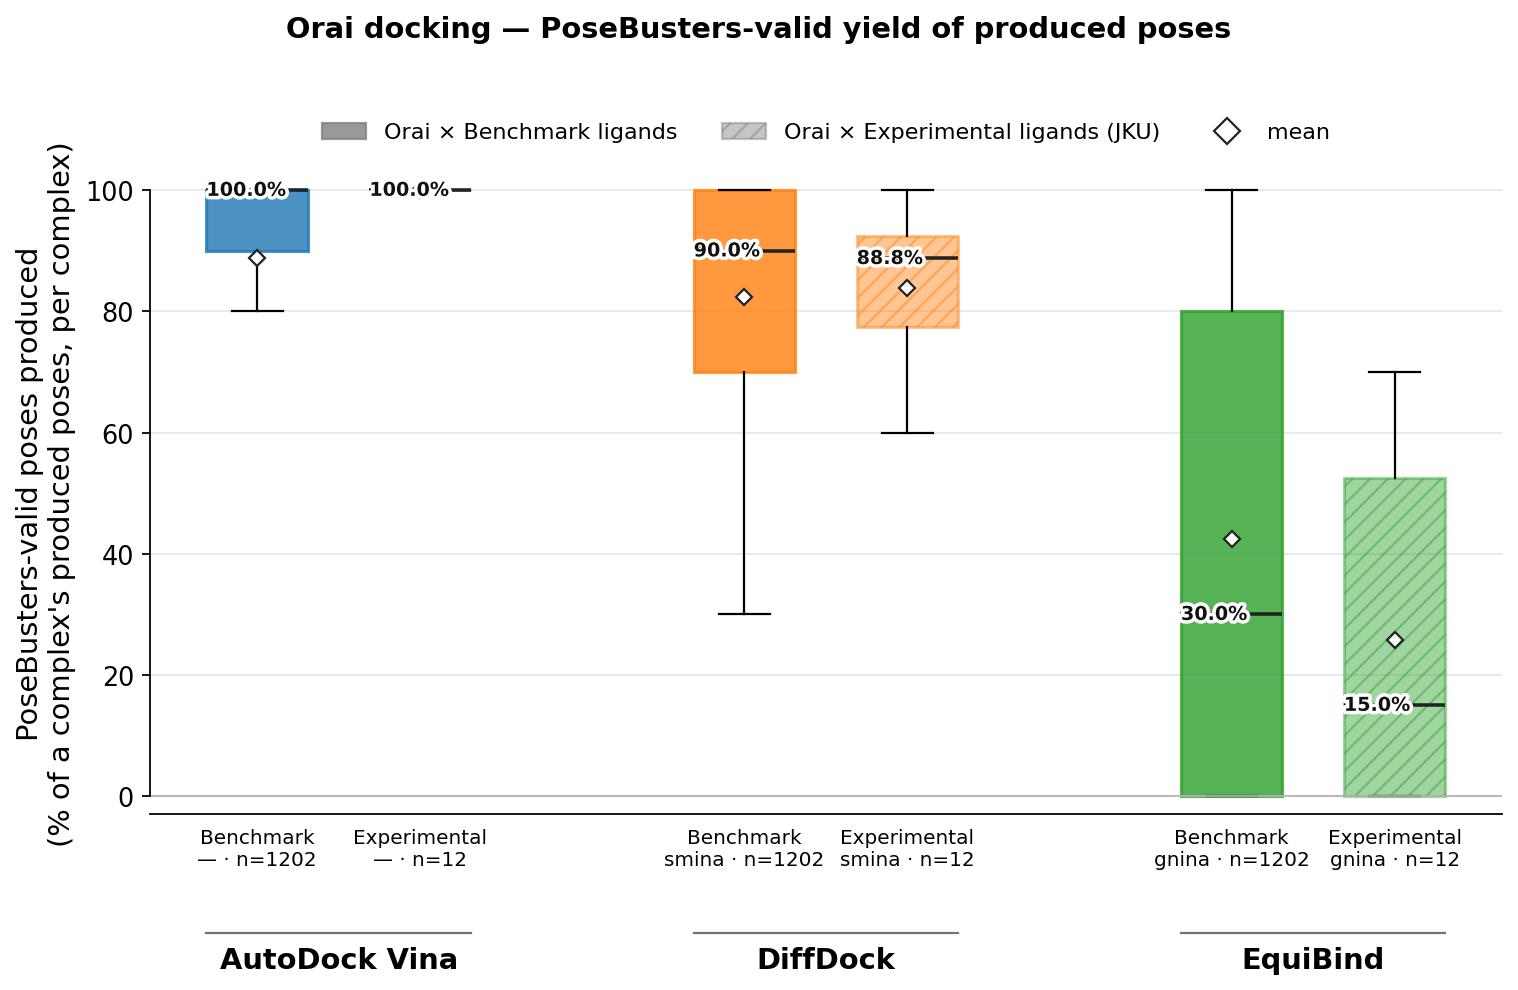
\includegraphics[width=\linewidth,height=0.78\textheight,keepaspectratio]{media/media/image13.png}
\caption{PoseBusters-valid yield of produced poses on Orai, benchmark against experimental ligands}\label{fig:results-r11}
\end{figure}

In Figure~\ref{fig:results-r11} AutoDock Vina is essentially perfect on the experimental ligands. Its median yield is 100\% on both sets, and on the twelve experimental complexes every produced pose passes, so that box collapses to a line at 100\%, against a benchmark mean of 88.9\% with a thin failure tail in which 3\% of complexes yield nothing. DiffDock is the most stable of the three, with medians of 90.0\% and 88.8\%, means of 82.4\% and 84.0\% and a tighter experimental spread, an interquartile range of 78 to 92\% against 70 to 100\%. EquiBind is the weakest tool in both sets, its median falling from 30.0\% to 15.0\% and its mean from 42.5\% to 25.8\%.

The ceiling and floor rates separate the tools more sharply than the medians do. On the benchmark AutoDock returns a fully clean complex, in which every produced pose is valid, for 72\% of complexes against 28\% for DiffDock, a 2.6-fold gap, since DiffDock sits in the 70 to 100\% band and rarely attains a perfect complex, and on the experimental ligands the same figures are 100\% and 25\%. The two tools are skewed in opposite directions, AutoDock being ceiling-bound with a mean below its median while EquiBind is floor-bound with a benchmark mean of 42.5\% above its median of 30\%, so no single central value describes both. EquiBind is best read as all-or-nothing rather than mediocre, its lower benchmark quartile pinned at zero with 27\% of complexes yielding nothing against 16\% fully clean, and on the experimental ligands both tails move the wrong way, 42\% of complexes yielding nothing and not one reaching a fully clean result, its best complex stopping at 70\%.

Per tool the sets were compared with an unpaired two-sided Mann-Whitney U test on the per-complex yields and Cliff\textquotesingle s \ensuremath{\delta}, oriented so that a positive value means the benchmark is higher. No tool shows a robust set difference. AutoDock is nominally cleaner on the experimental ligands, \ensuremath{\delta} = \ensuremath{-}0.28 at p = 0.033, but that contrast does not survive Holm correction across the three tools (p = 0.098) and is driven entirely by the benchmark\textquotesingle s small failure tail against a perfect twelve of twelve. DiffDock is indistinguishable across the sets, \ensuremath{\delta} = \ensuremath{-}0.001 at p = 0.99, and EquiBind trends better on the benchmark without reaching significance, \ensuremath{\delta} = +0.26 at p = 0.12.

The comparison is limited by the size and the chemistry of the experimental set, namely three ligands against 308, so the tests have little power and the non-significant results mean that no difference was detected rather than that none exists. Both EquiBind columns now use the same gnina refiner, so its cross-set contrast is no longer confounded by refiner choice.

In summary, the ordering AutoDock Vina, DiffDock and EquiBind is preserved for physical validity in both Orai ligand panels. This is consistent with, but does not prove, transfer from the calibration benchmark because the experimental panel contains only three ligands. AutoDock output needs little geometric repair, DiffDock is mostly valid after smina refinement, and EquiBind requires strict validity screening even after gnina optimisation. No between-panel contrast survives multiplicity correction.

\hypertarget{near-nativeness}{%
\subsection{\texorpdfstring{Near-Nativeness }{Near-Nativeness }}\label{near-nativeness}}

The Orai1 target has no ligand-bound reference, so RMSD to a native pose cannot be computed. Accuracy is therefore replaced by an operational placement rule. A pose is counted as usable only when it is PoseBusters-valid, remains associated with the receptor surface and lies outside the R91-E106 transmembrane exclusion slab. This rule focuses the analysis on an outer-pore hypothesis. It is not a near-native analogue or experimental ground truth.

\begin{figure}[!htbp]
\centering

\includegraphics[width=\linewidth,height=0.78\textheight,keepaspectratio]{media/media/image14.png}
\caption{Orai Fr300 with docked ligands and transmembrane exclusion}\label{fig:results-r12}
\end{figure}

Figure~\ref{fig:results-r13} reports the percentage of produced poses that are PoseBusters-valid, remain on the receptor and lie outside the exclusion slab, for twelve experimental units and 1,202 successfully processed control units.

\begin{figure}[!htbp]
\centering
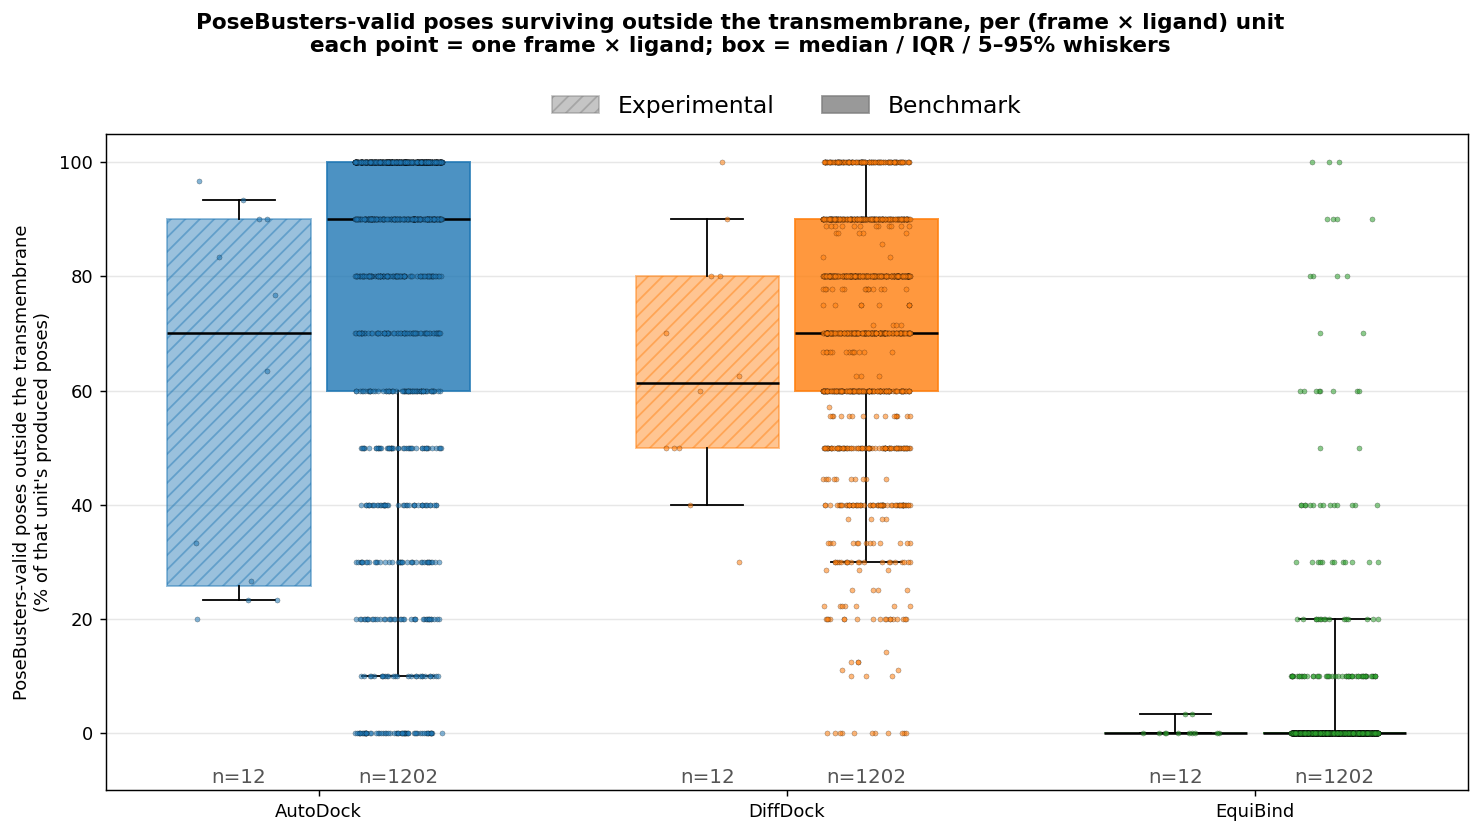
\includegraphics[width=\linewidth,height=0.78\textheight,keepaspectratio]{media/media/image43.png}
\caption{Usable pose yield per frame-ligand unit. Each point is one Orai frame paired with one ligand}\label{fig:results-r13}
\end{figure}

Each tool is capped at its top-10 ranked poses per unit, so the two sets sit on one comparable axis. AutoDock Vina gives the highest usable yield, a benchmark median of 90\% of produced poses against an experimental median of 70\%, with interquartile ranges of 60 to 100\% and 67.5 to 82.5\% and means of 77.0\% and 68.3\%. DiffDock follows at 70\% and 61.2\%, with spreads of 60 to 90\% and 50 to 80\% and means of 70.8\% and 63.5\%. EquiBind is degenerate in both sets, its median and both quartiles pinned at zero and its mean only 2.9\% on the benchmark and 0.8\% on the experimental ligands.

Tested at the honest unit with an unpaired two-sided Mann-Whitney U and Cliff\textquotesingle s \ensuremath{\delta}, no tool separates the two ligand sets. AutoDock trends towards the benchmark (U = 9540.5, \ensuremath{\delta} = +0.32) and DiffDock likewise (U = 8808.5, \ensuremath{\delta} = +0.22), but neither survives Holm correction across the three tools (p = 0.131 and 0.366), and EquiBind shows nothing (\ensuremath{\delta} = +0.02, p = 0.830). The pooled pose-level counterpart is only marginally stronger, AutoDock\textquotesingle s gap of 8.6\% giving an uncorrected Fisher p of 0.029 that likewise fails correction (p = 0.088), with DiffDock at 7.4\% and EquiBind at 2.0\% clearly non-significant. On this metric, therefore, both viable tools behave the same way on the experimental ligands as on the benchmark library, which is the generalisation evidence the section is looking for.

\begin{figure}[!htbp]
\centering
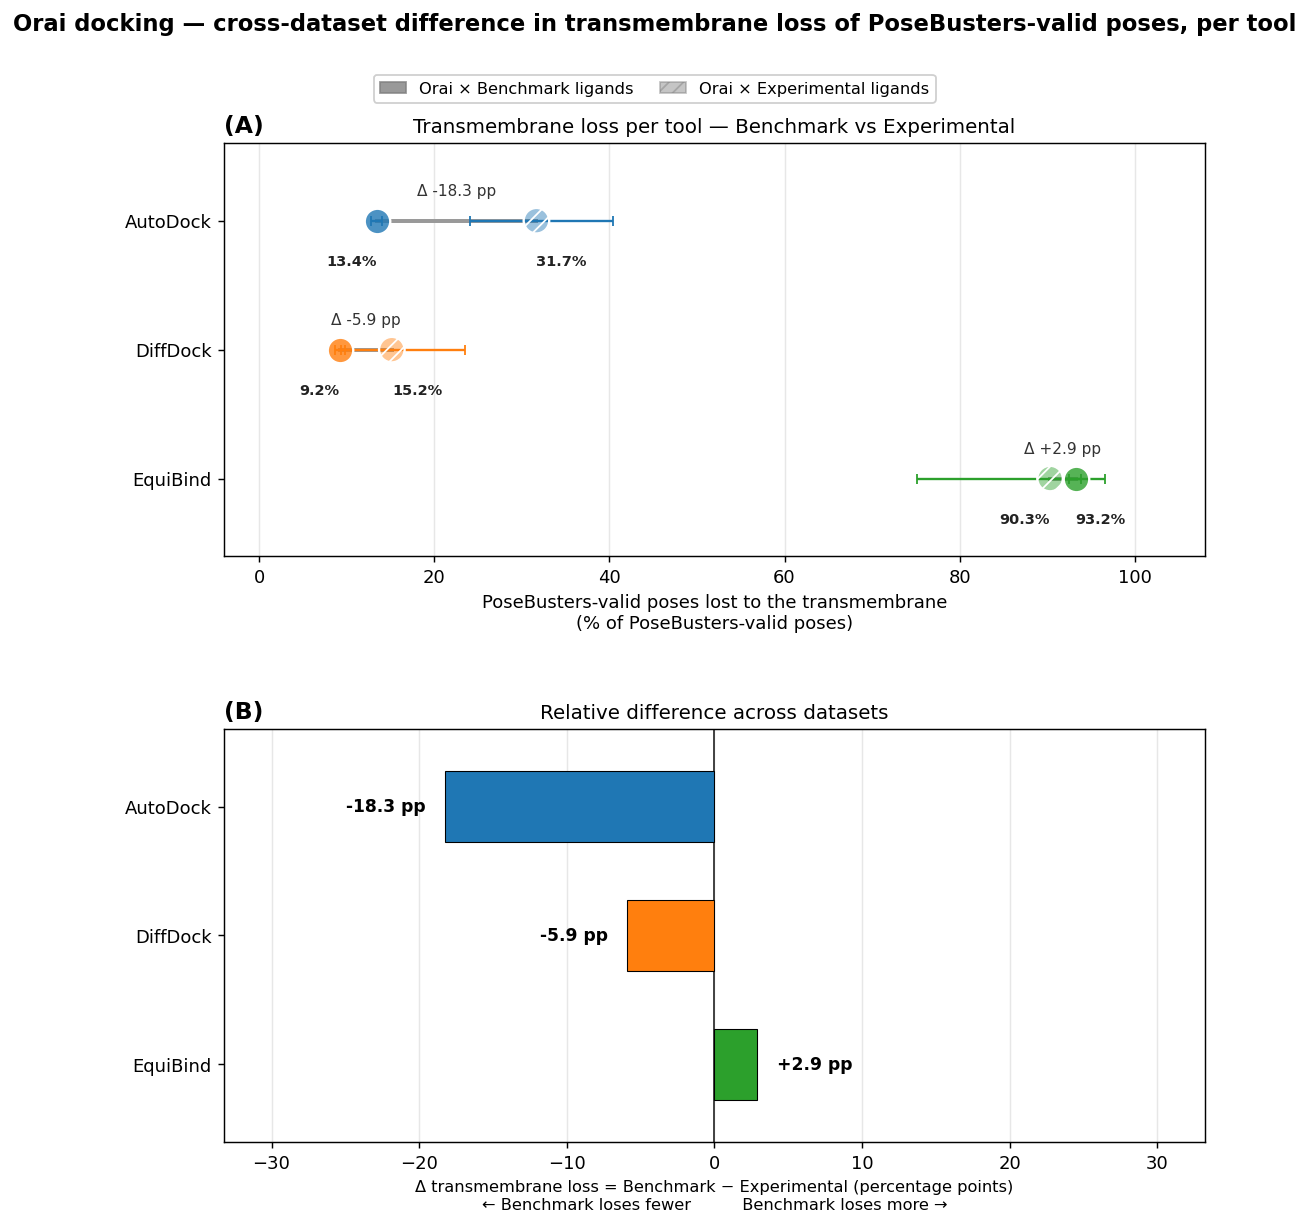
\includegraphics[width=\linewidth,height=0.78\textheight,keepaspectratio]{media/media/image15.png}
\caption{Transmembrane loss of PoseBusters-valid poses, benchmark against experimental ligands. Panel (A) loss rate per tool as pooled pose-level proportions with Wilson 95\% intervals. Panel (B) Difference per tool as benchmark minus experimental}\label{fig:results-r14}
\end{figure}

Figure~\ref{fig:results-r14} describes the share of already PoseBusters-valid poses that lies inside the transmembrane slab. AutoDock Vina loses 13.4\% of valid control-panel poses (1,433 of 10,686) and 31.7\% of experimental poses (38 of 120). DiffDock loses 9.2\% (874 of 9,487) and 15.2\% (15 of 99), respectively, while EquiBind loses 93.2\% and 90.3\% (28 of 31 experimental valid poses). Because poses are clustered within frame-ligand units, these pose-level contrasts are descriptive and their nominal tests should not be treated as independent biological replication.

Figures~\ref{fig:results-r13} and \ref{fig:results-r14} separate validity from conditional placement. DiffDock loses a smaller share of its already valid control poses to the transmembrane slab than AutoDock Vina (9.2\% versus 13.4\%), whereas AutoDock Vina has the higher net usable yield because it generates more valid poses. EquiBind fails both the receptor-association and non-pore placement requirements. Of 31 valid experimental poses, 28 are in the slab, two are off-protein and one is usable. The combined placement screen, rather than physical validity alone, is therefore decisive for this Orai1 protocol.

Two limits bound these comparisons. The transmembrane-loss rates are pooled pose-level tests that treat correlated poses within a unit as independent, so they overstate significance and are descriptive only. Their honest per-unit sibling, the usable-yield test above, is non-significant for all three tools, so AutoDock\textquotesingle s 18.3\% loss gap should be read as a pooled description rather than as a generalisation claim. The cross-set differences are also reported as absolute differences rather than ratios, because the experimental denominator rests on three ligands and at most twelve units, which makes a ratio such as the apparent 0.42-fold reduction in loss unstable. Since the four frames are snapshots of one receptor, even the per-unit test is anti-conservative for the question of generalisation to new ligands.

\hypertarget{cross-tool-clustering-1}{%
\subsection{Cross-Tool Clustering}\label{cross-tool-clustering-1}}

The clustering approach is applied per MD frame and ligand pair, one pose cloud per frame, ligand and tool, to ask whether the three toolchains point to the same region of Orai and how well formed each tool\textquotesingle s own cloud is. Since frames of the same ligand are snapshots of one receptor-ligand system rather than independent observations, the pooled medians below are mildly pseudoreplicated. A frame-robust summary that collapses each ligand to the median over its frames first gives 37.7\angstrom{} against the pooled 29.9\angstrom{} on the experimental ligands and 30.2 \angstrom{} against 29.5 \angstrom{} on the benchmark, so the benchmark figure is stable and the experimental one shifts upwards with only three ligands to average over.

\begin{figure}[!htbp]
\centering
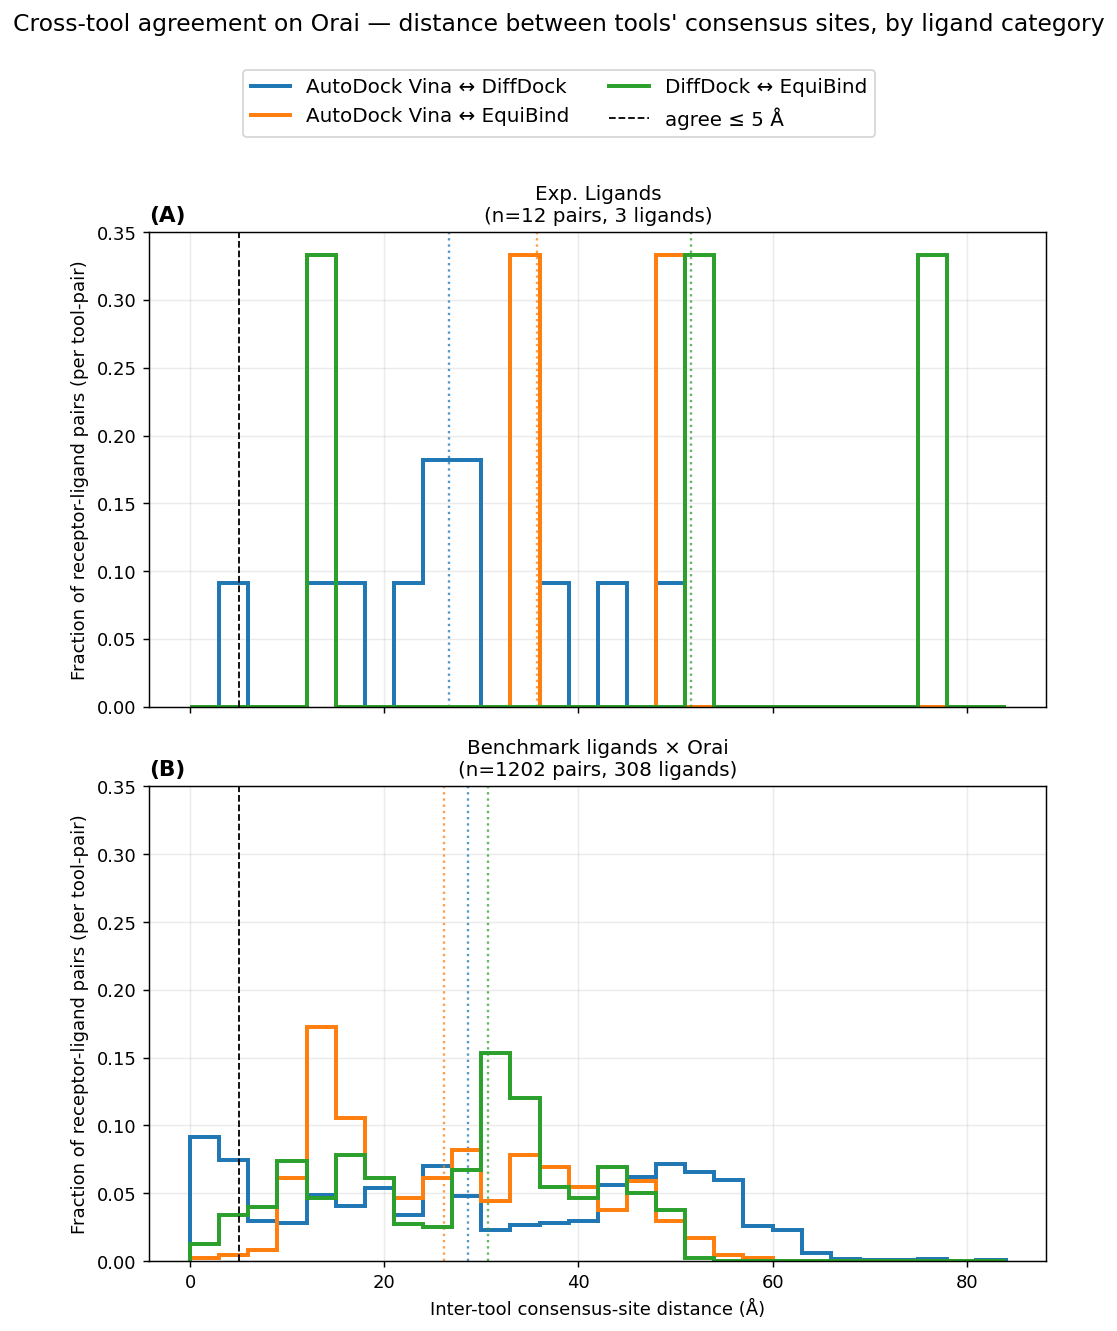
\includegraphics[width=\linewidth,height=0.78\textheight,keepaspectratio]{media/media/image16.png}
\caption{Distribution of inter-tool consensus-site distances on Orai. Step histograms per tool pair}\label{fig:results-r15}
\end{figure}

Figure~\ref{fig:results-r15} shows the distribution of the distance between each pair of tools\textquotesingle{} consensus sites for the two ligand sets. Almost nothing falls left of the 5 \angstrom{} agreement line. Distances run from a few ångströms to more than 80\angstrom{}, since candidate sites scatter along the elongated Orai pore, and the per-pair medians sit at 26 to 31 \angstrom{} on the benchmark ligands against 27 to 52 \angstrom{} on the experimental ones. Agreement therefore has to be read from the continuous distance and the per-pair rate rather than from a binary consensus flag, which is 0\% in both sets.

\begin{figure}[!htbp]
\centering

\includegraphics[width=\linewidth,height=0.78\textheight,keepaspectratio]{media/media/image17.png}
\caption{Cross-tool agreement on Orai. Panel (A) gives the inter-tool consensus-site distance per tool pair and pooled over all pairs, hatched for the experimental ligands and solid for the benchmark set. Panel (B) gives the percentage of pairs within the 5\angstrom{} threshold, per tool pair and pooled over all pairs, with Wilson 95\% intervals and the underlying counts}\label{fig:results-r16}
\end{figure}

No pairing differs significantly between the ligand sets. DiffDock and EquiBind show the largest gap, 51.6\angstrom{} on the experimental ligands against 30.7\angstrom{} on the benchmark with \ensuremath{\delta} = \ensuremath{-}0.45, yet at eleven and three usable experimental pairs the contrast does not survive Holm correction (p = 0.708), and AutoDock against EquiBind (35.7\angstrom{} against 26.1 \angstrom{}, \ensuremath{\delta} = \ensuremath{-}0.19) and AutoDock against DiffDock (26.6\angstrom{} against 28.6\angstrom{}, \ensuremath{\delta} = +0.10) are flat. The agreement rates tell the more important story. AutoDock and DiffDock land within 5 \angstrom{} in 15\% of benchmark pairs, 173 of 1 190, and in one of eleven experimental pairs, whereas every EquiBind pairing stays at or below 4\%, namely 2 of 475 against AutoDock and 17 of 475 against DiffDock, with none at all on the experimental ligands, and all rate differences give a Fisher p of 1.000. Pooled over all three pairings, agreement within 5 \angstrom{} is 9\% on the benchmark, 192 of 2 140, and one of seventeen on the experimental ligands. Strict three-way agreement is 0\% in both sets. The only real agreement channel is therefore AutoDock against DiffDock, and any consensus site on Orai is in practice a question about those two tools alone.

\begin{figure}[!htbp]
\centering
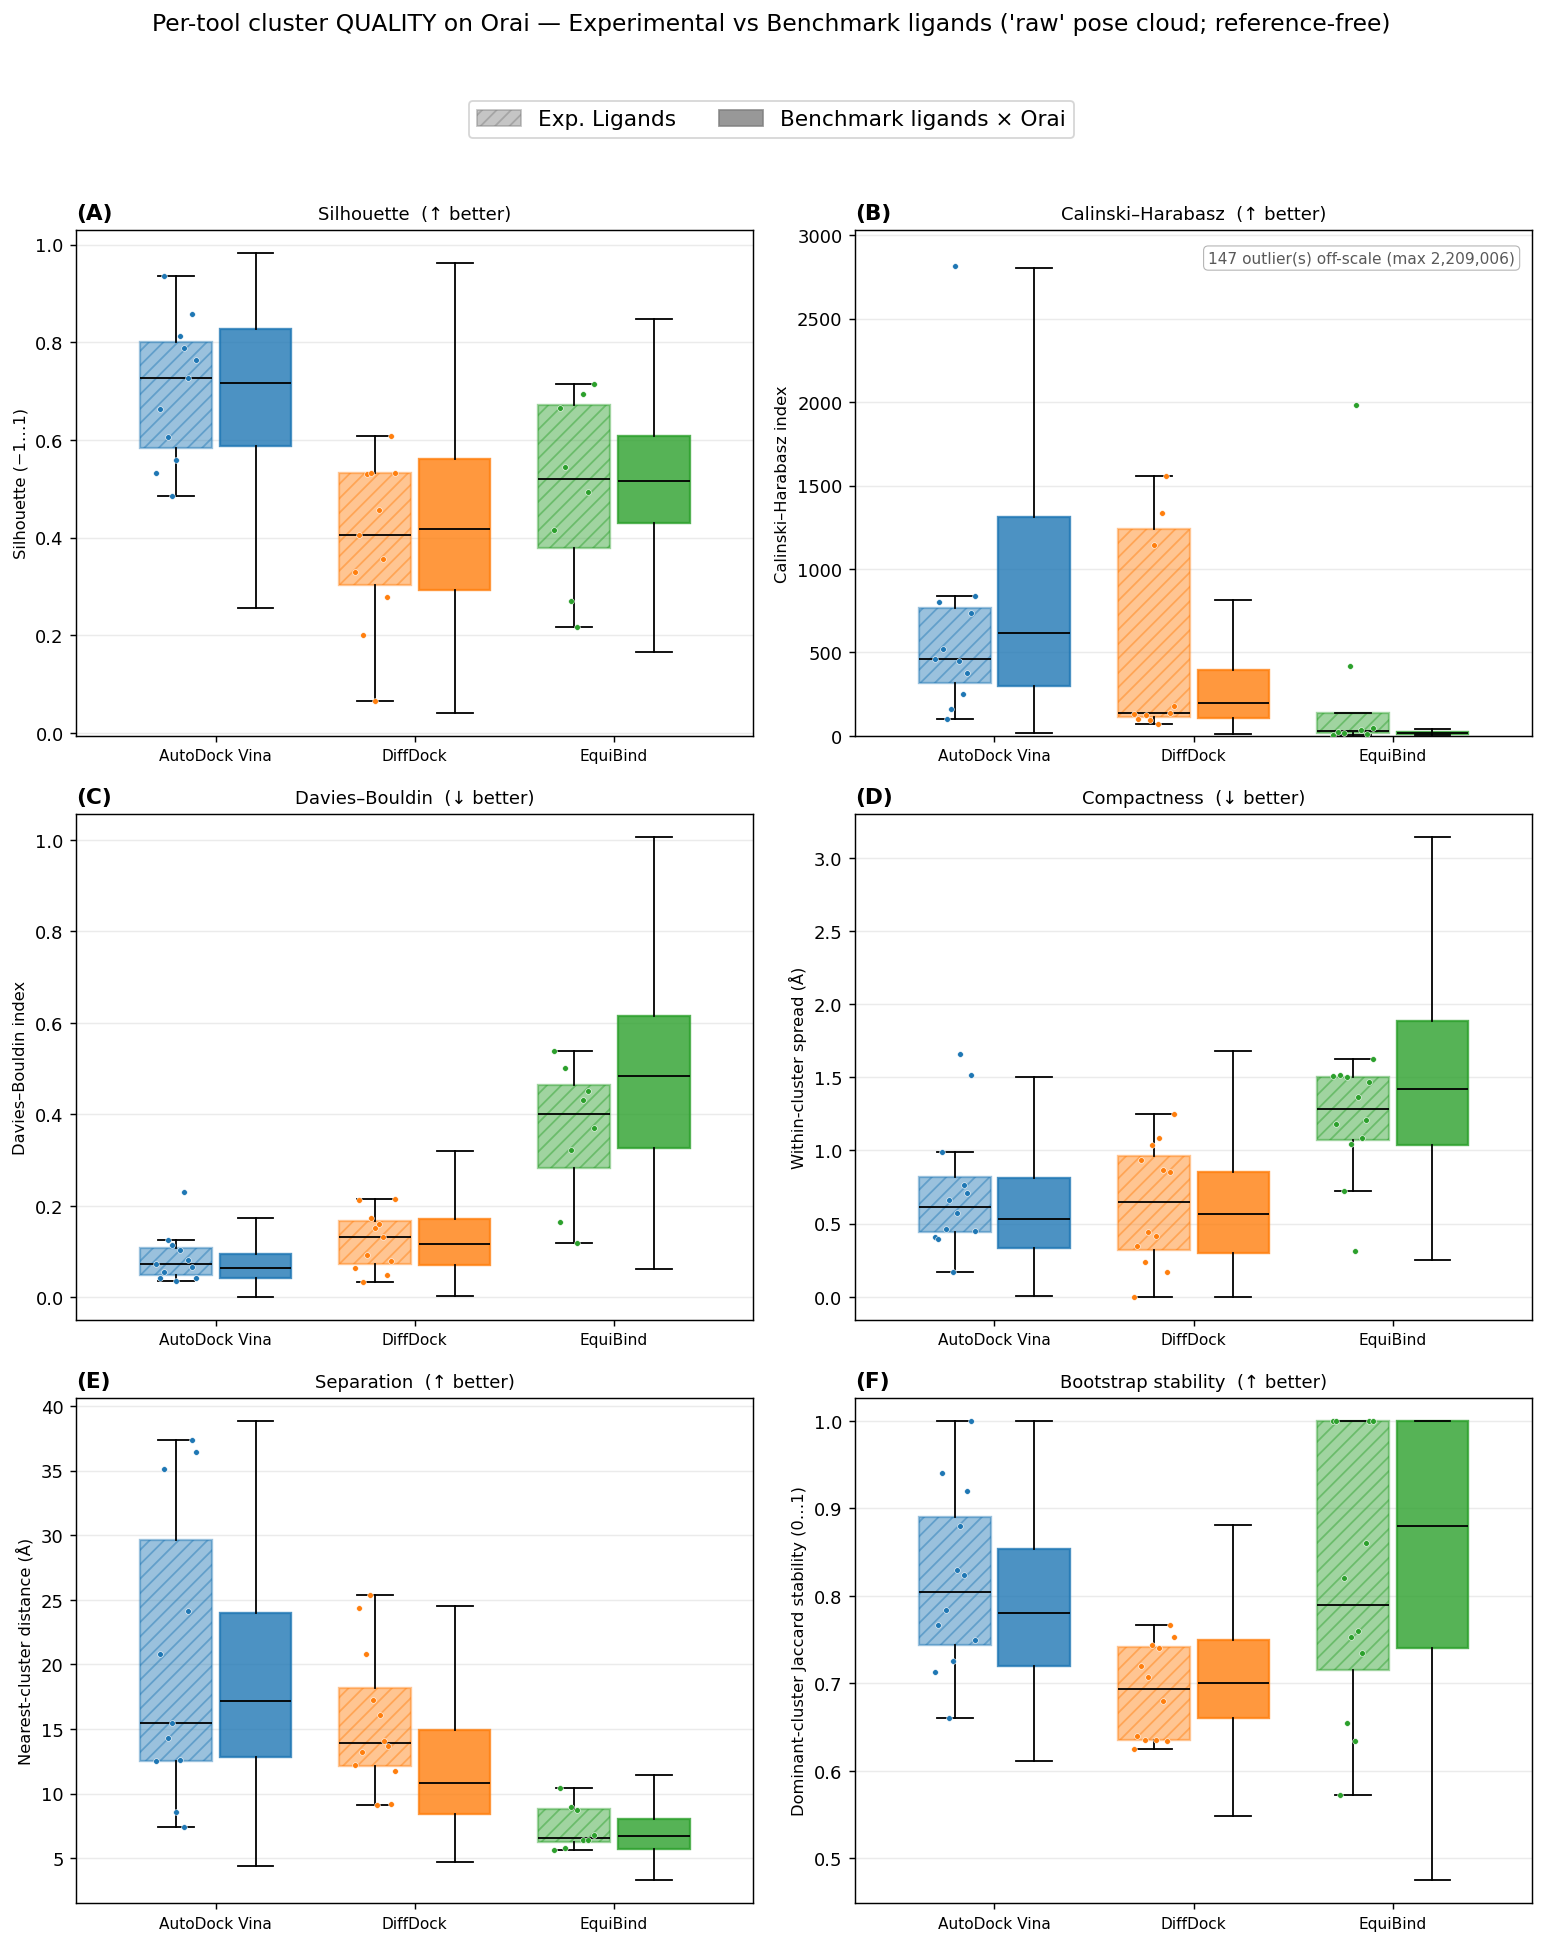
\includegraphics[width=\linewidth,height=0.78\textheight,keepaspectratio]{media/media/image18.png}
\caption{Reference-free cluster quality per tool on Orai}\label{fig:results-r17}
\end{figure}

AutoDock Vina forms the most compact and separated pose clouds in both panels, while EquiBind forms the loosest clouds and often collapses into one diffuse mode. High bootstrap stability in such a degenerate case reflects reproducibility of the same broad cloud rather than accurate site resolution. No experimental-versus-control contrast across the reported cluster metrics survives Holm correction, but the experimental panel contains only three ligands. The justified statement is therefore that no panel difference was detected at the available power. The result does not establish equivalence or validate the control panel as a stand-in.

\begin{figure}[!htbp]
\centering

\includegraphics[width=\linewidth,height=0.78\textheight,keepaspectratio]{media/media/image19.png}
\caption{Effect of validity and placement filtering on cluster compactness. Within-cluster spread per tool for the raw pose cloud against the filtered cloud of PoseBusters-valid poses outside the transmembrane pore, panel (A) for the experimental ligands and panel (B) for the benchmark set, paired within each frame-ligand pair}\label{fig:results-r18}
\end{figure}

Filtering to poses that are PoseBusters-valid and outside the pore does not tighten the clouds. AutoDock moves in the tighter direction with a rank-biserial effect of \ensuremath{-}0.53 but does not reach significance (Holm-corrected p = 0.641), DiffDock barely moves at \ensuremath{-}0.13, and EquiBind cannot be tested at all, since too few of its poses survive the gate, which is itself the clearest statement of its weakness on this target. The only near-significant change is a gain in DiffDock\textquotesingle s dominant-cluster stability, rank-biserial +0.89 at a corrected p of 0.059. The wide scatter along the pore is therefore intrinsic to how the tools sample rather than an artefact of invalid or mislocated poses that filtering could clean away.

In summary, the tools do not provide a reliable consensus site on Orai1. Pairwise sites differ by roughly 30 \angstrom{} at the median, and agreement within 5 \angstrom{} reaches at most 15\%. AutoDock Vina forms the tightest and best-separated pose clouds, but precision is not evidence of accuracy without a reference. None of the experimental-versus-control contrasts in agreement or cluster quality survives correction. The preserved descriptive ordering supports cautious use of the control panel for these proxies, but it does not validate equivalence.

\protect\hypertarget{_Toc235735939}{}{}

\hypertarget{interaction-and-contact-analysis-1}{%
\subsection{Interaction and Contact Analysis}\label{interaction-and-contact-analysis-1}}

All poses entering the analysis are PoseBusters-valid and outside the transmembrane slab, capped at each tool\textquotesingle s top three ranked poses per frame-ligand unit, and both ligand sets were docked into the same four frames, so the residue axis is directly comparable. PandaMap typed every contact at residue level into fifteen interaction classes. After filtering, the experimental set contributes 33 poses from 11 complexes for AutoDock and 36 from 12 for DiffDock, against 3 332 and 3 485 benchmark poses, whereas EquiBind retains a single experimental pose against 231, so every EquiBind figure below is non-interpretable and is reported only for completeness. Poses within a complex are correlated, so the figures display pose-level values, but every contact-count and type-profile significance test aggregates to the per-complex mean first, before an unpaired Mann-Whitney U test with Cliff\textquotesingle s \ensuremath{\delta} oriented so that a positive value means the benchmark is higher. The prose therefore quotes the pose-level medians shown on the plots as the descriptive summary and the per-complex-mean values alongside each \ensuremath{\delta} as the inferential unit.

\begin{figure}[!htbp]
\centering

\includegraphics[width=\linewidth,height=0.78\textheight,keepaspectratio]{media/media/image20.png}
\caption{Total protein-ligand contacts per pose on Orai}\label{fig:results-r19}
\end{figure}

Figure~\ref{fig:results-r19} compares total contacts per pose between the two ligand panels; the pose-level median is printed on each box. AutoDock Vina trends toward denser contacts for the experimental ligands, its median rising from 23 for the benchmark set to 28 for the experimental set, whereas DiffDock edges the other way, from 15 to 14. Neither trend survives testing one level up on the per-complex mean, which removes the pose pseudoreplication: AutoDock gives Cliff\textquotesingle s \ensuremath{\delta} = \ensuremath{-}0.31 at a Holm-adjusted p = 0.235 (per-complex-mean medians 23.3 for the benchmark against 30.0 for the experimental set), and DiffDock \ensuremath{\delta} = +0.11 at p = 0.526 (15.7 against 14.3). EquiBind contributes only one usable experimental pose. No difference in total contact count is detected at the available power, which is not evidence that the panels have equivalent contact intensity.

\begin{figure}[!htbp]
\centering

\includegraphics[width=\linewidth,height=0.9\textheight,keepaspectratio]{media/media/image21.png}
\caption{Interaction-type profile on Orai. Mean count per pose of each PandaMap interaction type}\label{fig:results-r20}
\end{figure}

Figure~\ref{fig:results-r20} gives the mean count per pose of each interaction type; as for the totals, the plotted bars are pose-level means and the values quoted below are the per-complex means that enter the tests. The rank order is preserved across the ligand sets for both mature tools, alkyl-\ensuremath{\pi}, hydrophobic contacts, hydrogen bonds and the \ensuremath{\pi} family dominating throughout, yet four differences are robust and chemically coherent. The benchmark ligands form more hydrogen bonds, 3.66 against 2.00 per pose for AutoDock and 2.47 against 0.97 for DiffDock, at corrected p of 0.004 and 5.6e-4 with \ensuremath{\delta} = +0.58 and +0.69. The blockers form more halogen bonds, 1.15 against 0.20 and 0.78 against 0.16, corrected below 1e-3 for both tools. Under AutoDock they are also markedly more hydrophobic, 5.70 against 3.13 with \ensuremath{\delta} = \ensuremath{-}0.75 at a corrected p of 1.4e-4, and richer in alkyl-\ensuremath{\pi} contacts, 6.12 against 4.01 at 0.027, while the charged classes, namely ionic, salt-bridge and attractive-charge contacts, appear only in its benchmark poses at 0.50 per pose each, also at 0.027. DiffDock moves in the same direction on the greasy and charged classes without reaching significance. The picture is a consistent chemotype signature rather than noise, since the real modulators are halogenated lipophilic compounds and the benchmark library is comparatively polar and hydrogen-bond driven.

\begin{figure}[!htbp]
\centering

\includegraphics[width=\linewidth,height=0.9\textheight,keepaspectratio]{media/media/image22.png}
\caption{Orai residue hot-spots}\label{fig:results-r21}
\end{figure}

Figure~\ref{fig:results-r21} turns from contact types to their location, reporting for the fifteen most frequently contacted Orai residues the percentage of a tool\textquotesingle s poses that touch each one. Both libraries concentrate on the same pocket residues, namely Asp110, Leu109, Gln108, Lys87, Arg83, Asp112 and Tyr115, and the divergences are confined to a hydrophobic sub-pocket. Under AutoDock the blockers engage Ala177 in 63.6\% of poses against 21.4\% of benchmark poses, Lys85 in 45.5\% against 16.9\% and Glu173 in 39.4\% against 20.2\%, while the benchmark ligands engage Trp76 more often, 28.4\% against 6.1\%. DiffDock echoes the pattern only weakly and in the opposite direction on Ala177, which its blocker poses never touch, and its own preference is for Tyr115. These are pose-level two-proportion tests and therefore pseudoreplicated, so they are descriptive support for the figure rather than inference, but the direction is consistent with the more hydrophobic type profile of the blockers.

\begin{figure}[!htbp]
\centering

\includegraphics[width=\linewidth,height=0.78\textheight,keepaspectratio]{media/media/image23.png}
\caption{Contact-fingerprint overlap between the two ligand sets}\label{fig:results-r22}
\end{figure}

Figure~\ref{fig:results-r22} summarises how far the two libraries agree on the residues they engage. Overlap is graded by tool, the residue-level Jaccard being 0.53 for AutoDock and 0.42 for DiffDock, and it falls to 0.27 and 0.28 once the interaction type must match as well, since the two libraries hit the same residues without always forming the same kind of contact there, which is the fingerprint-level echo of the hydrogen-bond against hydrophobic shift above. AutoDock shares 33 characteristic residues between the libraries and DiffDock 17, whereas EquiBind shares none, its single experimental pose leaving a Jaccard of zero that carries no meaning. One reading trap deserves flagging. The 10\% threshold is an absolute count, roughly four poses for the experimental set against several hundred for the benchmark, and the diverse benchmark ligands spread their contacts across many residues while the three repeatedly docked blockers concentrate theirs, so the experimental-only count exceeding the benchmark-only count, 22 against 7 for AutoDock, is an artefact of set size and homogeneity rather than evidence of promiscuity. The shared set and the per-residue frequencies are the robust readings.

The surviving blocker poses show partial concordance with published pharmacology. Synta-66 has been mapped to the outer TM1/TM3 interface adjacent to the E106 selectivity filter \cite{ref070}, \cite{ref071}. AutoDock Vina enrichment at Ala177 is compatible with TM3 involvement, while DiffDock contacts at Glu106 are compatible with a filter-adjacent hypothesis. These observations make the poses biologically interpretable, but contacts contributed by different tools cannot be combined to validate one binding mode. The remaining frequent residues define plausible hypotheses for mutagenesis or ligand-bound simulation.

The comparison is unpaired and confounded by chemistry, so the contact-type split characterises chemotypes rather than tool skill. Without a cognate structure, literature concordance remains partial and some retained poses are still anatomically implausible. Pose-level residue tests are pseudoreplicated, the experimental arm contains three ligands, and EquiBind contributes only one usable experimental pose. Effect sizes and qualitative agreement with pharmacology therefore carry more weight than nominal p-values.

Taken together, the Orai1 analysis preserves the benchmark ordering on net usable yield. AutoDock Vina is physically clean and retains 60 to 75\% of poses per ligand under the operational placement rule, with a median usable yield of 70\%. DiffDock follows at a median validity of 88.8\% and usable yield of 61.2\%. Conditional on already valid control poses, it has a lower transmembrane-loss rate than AutoDock Vina. EquiBind has a median experimental validity of 15\%, and 30 of its 31 valid poses fail the on-receptor, non-pore placement rule, leaving one usable pose out of 120.

Three methodological conclusions follow. First, chemical validity alone overstates usefulness on a channel target, since a tool can be geometrically flawless and still dock into the ion-conduction pathway, so usable yield rather than raw validity is the defensible headline metric and the placement filter is what exposes EquiBind. Second, cross-tool consensus is not available as a confidence signal here, because the three tools disagree about where these ligands bind by roughly 30 \angstrom{} at the median, agree within 5 \angstrom{} in at best 15\% of pairs and never as a trio, and filtering to valid, correctly placed poses does not tighten that scatter, so it is intrinsic to how the tools sample an elongated pore rather than an artefact of poor poses. Third, the surviving poses do carry chemical signal. Both libraries engage the same pocket residues, yet the real modulators are measurably more hydrophobic and halogen-rich and less hydrogen-bonded than the benchmark ligands, and they lean into an Ala177, Glu173 and Lys85 hydrophobic sub-pocket, which under AutoDock and DiffDock together reconstructs the outer TM1 and TM3 region adjacent to the selectivity filter where the Synta-66 site has been mapped experimentally.

The cross-panel comparison is reassuring only in a limited descriptive sense. No experimental-versus-control contrast survives correction for validity, usable yield, inter-tool agreement, cluster quality or total contact density, but the experimental panel is too small to establish equivalence. Interaction-type differences are consistent with the more hydrophobic, halogen-rich experimental chemotypes, and residue-level fingerprint overlap is moderate for AutoDock Vina and DiffDock. For Orai1, the practical recommendation is to retain AutoDock Vina and refined DiffDock as separate hypothesis generators, prioritise poses that satisfy the validity and placement rules and agree with independent pharmacology, and omit EquiBind in its present configuration. Sparse overlap between the two viable tools should not itself be treated as validation.

\protect\hypertarget{_Toc235735941}{}{}

\hypertarget{dataset-summary}{%
\section{Dataset Summary}\label{dataset-summary}}

Across the 303 common calibration complexes retained from the 308-complex source benchmark, AutoDock Vina is the strongest configured pipeline on the primary combined endpoint, physical validity, crystal-pocket recovery and native-interaction recovery. This ordering describes the workflows as configured, not the method classes under matched information. On this calibration set AutoDock Vina searched a crystal-ligand-centred box while DiffDock and EquiBind docked blind, an asymmetry that most directly aids AutoDock Vina on crystal-pocket recovery and the placement component of the combined endpoint. DiffDock is consistently second and is limited chiefly by selection, because acceptable poses often occur within a shallow top-15 pool but are not ranked first. EquiBind remains weakest and is limited chiefly by generation, placement and raw geometry. On Orai1, AutoDock Vina has the highest net usable yield, although DiffDock loses a smaller conditional share of already valid control poses to the transmembrane slab.

Two conclusions cut across the datasets. First, post-hoc minimisation makes many learned poses physically admissible but does little to correct gross placement. Second, the residual bottleneck differs by tool. DiffDock leaves substantial ranking headroom, while EquiBind often fails to sample a usable placement at all. It is therefore not accurate to describe all remaining loss as selection rather than search.

The calibration analysis carries the greater inferential weight because it contains 303 crystal-referenced complexes. The Orai1 arm contains three ligands and twelve correlated frame-ligand units without a cognate pose. Its value lies in reference-free workflow diagnosis and partial concordance with filter-adjacent pharmacology, not in a statistically powered estimate of prospective accuracy.

\hypertarget{pose-production-costs}{%
\section{Pose Production Costs}\label{pose-production-costs}}

Accuracy and validity say nothing about what a result costs. The relevant efficiency measure is not throughput but the compute spent per usable result, so cost is expressed per pose that clears the deployment bar, namely PoseBusters-valid and within 2 \angstrom{} of the crystal ligand. Two views follow, the wall-clock a user waits for and the hardware resource a cluster bills. All docking ran on a single workstation. That machine used an Intel Core i9-14900HX processor with 32 hardware threads, an NVIDIA GeForce RTX 4070 Laptop GPU with 8 GB of video memory, and 32 GB of system memory. AutoDock Vina ran multi-threaded on the processor at exhaustiveness 32, while DiffDock and EquiBind ran on the GPU.

Figure~\ref{fig:results-r23} gives the wall-clock cost per qualifying pose, one value per complex, over the complexes for which a tool produced at least one such pose.

\begin{figure}[!htbp]
\centering

\includegraphics[width=\linewidth,height=0.78\textheight,keepaspectratio]{media/media/image24.png}
\caption{Wall-clock seconds per qualifying pose, where a qualifying pose is PoseBusters-valid and within 2 \angstrom{} of the crystal ligand}\label{fig:results-r23}
\end{figure}

The cost ordering is AutoDock Vina, then EquiBind, then DiffDock, and every difference is large and significant. Medians are 3.5 s per qualifying pose for AutoDock (interquartile range 1.0 to 7.3 s, 261 complexes), 8.4 s for EquiBind (3.2 to 21.8 s, 63 complexes) and 50.9 s for DiffDock (15.6 to 143.9 s, 162 complexes). On the 47 complexes where all three succeed the paired tests confirm the ordering (Friedman \ensuremath{\chi}\textsuperscript{2} = 37.1, p \textless{} 1e-8, Kendall W = 0.39, all pairs surviving Holm correction with rank-biserial effects of \ensuremath{-}0.86, \ensuremath{-}0.63 and +0.74), and DiffDock costs 7.0 times as much per usable pose as AutoDock {[}2.5 to 18.8{]} against EquiBind\textquotesingle s 2.5 times.

Cost climbs as the quality bar tightens, most steeply for the learned tools. From any pose through valid to valid and near-native the median runs 0.3, 0.3 and 3.5 s for AutoDock, 8.1, 10.4 and 50.9 s for DiffDock and 0.9, 1.2 and 8.4 s for EquiBind, while the contributing complexes fall from 293 to 261, 162 and 63. Fewer qualifying poses spread the same fixed docking wall further, and many complexes yield none at all. EquiBind\textquotesingle s competitive unit cost is an artefact of the latter, since its 8.4 s is averaged over the 63 complexes in which it succeeds and it fails in the remaining 230.

Figure~\ref{fig:results-r24} removes parallelism from the comparison, reporting the hardware resource consumed per qualifying pose separately for CPU and GPU, on the same near-native and valid criterion as Figure~\ref{fig:results-r23}.

\begin{figure}[!htbp]
\centering

\includegraphics[width=\linewidth,height=0.78\textheight,keepaspectratio]{media/media/image25.png}
\caption{Hardware resource per near-native valid pose, that is per pose that is PoseBusters-valid and within 2 \angstrom{} of the crystal ligand}\label{fig:results-r24}
\end{figure}

On this axis the wall-clock story inverts. AutoDock consumes 218.8 CPU-core-seconds and no GPU time per qualifying pose, DiffDock 51.1 GPU-seconds and 2.9 CPU-core-seconds, and EquiBind 790.5 CPU-core-seconds with 2.0 GPU-seconds. AutoDock looked cheapest in wall-clock precisely because it spreads work over 32 threads, and that parallelism is the cost. EquiBind is the most expensive on the CPU axis, roughly 3.6 times AutoDock, and is penalised twice over, performing the most CPU work and converting it into the fewest qualifying poses, 317 (EquiBind) against 610 (AutoDock Vina) and 1 526 (DiffDock). DiffDock is the only real GPU consumer, so it is CPU-cheap only in the sense of having offloaded the work, and its larger pose pool also flatters its per-pose figures.

Three caveats bound these figures. The wall-clock comparison is cross-hardware, AutoDock running multi-threaded on CPU against a single GPU for the learned tools, so it measures elapsed time rather than identical work. The resource values are order-of-magnitude costs, since AutoDock\textquotesingle s CPU-core-seconds assume the full 32 threads and EquiBind\textquotesingle s wall time is a best-configuration estimate. The resource panel carries no inferential test by design, being a pooled aggregate rather than a per-complex distribution, and the tools do differ sharply on its denominator (Cochran\textquotesingle s Q = 97.0, p \textless{} 1e-21, at pooled validity rates of 94.8\%, 78.7\% and 52.3\%).

In summary, AutoDock Vina is the most efficient configured pipeline in elapsed time and has the highest success coverage (261 of 293 timing-complete complexes). DiffDock does not improve cost-effectiveness for this cognate re-docking setup, and EquiBind\textquotesingle s apparently lower median elapsed cost is conditional on only 63 successful complexes. Hardware-resource conclusions remain currency-specific. GPU time is the main cost for DiffDock, while CPU time dominates AutoDock Vina and especially EquiBind.

\hypertarget{discussion}{%
\chapter{\texorpdfstring{Discussion }{Discussion }}\label{discussion}}

\hypertarget{principal-findings-and-scope-of-inference}{%
\section{Principal Findings and Scope of Inference}\label{principal-findings-and-scope-of-inference}}

This study compared AutoDock Vina, DiffDock and EquiBind in two deliberately different settings, namely crystallographic re-docking on 303 calibration complexes retained from the 308-complex PoseBusters benchmark, and reference-free docking of three Orai1 modulators into four molecular-dynamics snapshots. The calibration benchmark provides the stronger evidence because every prediction can be tested against an experimental pose. In that setting, AutoDock Vina was the most reliable configured pipeline on the primary combined endpoint, physical validity, native-pocket recovery and interaction recovery. Refined DiffDock ranked second and retained useful conformational and sampling ability, whereas refined EquiBind was limited by low raw physical validity and weak placement. The Orai1 case broadly preserved this ordering under the study\textquotesingle s operational validity and placement rules, but the absence of a ligand-bound Orai1 structure means that it cannot establish which predicted binding mode is correct.

The appropriate interpretation is therefore narrower than a general contest between artificial intelligence and physics. The results show that AutoDock Vina outperformed the tested DiffDock-L and EquiBind pipelines under this study\textquotesingle s preparation, search, ranking, refinement and evaluation settings. They do not show that classical docking universally outperforms current AI docking. EquiBind and the evaluated DiffDock version represent earlier learned architectures, while more recent diffusion, co-folding and hybrid systems report better performance when pockets are specified, receptor flexibility is represented and structural relaxation is included \cite{ref012}, \cite{ref013}, \cite{ref031}, \cite{ref064}, \cite{ref069}. Conversely, current similarity-controlled analyses continue to show that aggregate accuracy can conceal reliance on training-set analogues and weak extrapolation to new pockets \cite{ref035}, \cite{ref063}, \cite{ref065}, \cite{ref069}. The principal contribution of this thesis is thus its separation of failure modes, namely sampling, ranking, physical validity and placement, rather than a permanent ranking of method classes.

The term physics-based also requires care. AutoDock Vina uses an empirical scoring function and an explicit search-and-optimisation procedure. It is not a full molecular-mechanics or free-energy simulation. In this thesis, physics-based is therefore an operational contrast with end-to-end learned pose generation. That distinction matters when interpreting the strong Vina result. It supports this classical search-and-score workflow, not a claim that a complete physical model of binding was evaluated.

\hypertarget{physical-validity-and-post-docking-optimisation}{%
\section{Physical Validity and Post-Docking Optimisation}\label{physical-validity-and-post-docking-optimisation}}

The largest initial separation between the tools occurred before RMSD was considered. AutoDock Vina produced 94.8\% PoseBusters-valid poses, compared with 23.9\% for raw DiffDock and 2.7\% for raw unguided EquiBind. Refinement substantially changed the usability of the learned outputs, because smina raised DiffDock validity to 78.7\%, while gnina raised unguided EquiBind validity to 52.3\%. These gains support the central PoseBusters argument that RMSD alone is insufficient, because a geometrically close ligand can still contain unrealistic bond geometry, steric overlap or intermolecular contacts \cite{ref035}. They are also consistent with broader benchmarking in which learned methods can lead on pose accuracy while classical methods retain an advantage in structural rationality, making combined accuracy-and-validity criteria more discriminating than RMSD alone \cite{ref013}, \cite{ref032}.

Refinement did not have the same practical effect for the two learned methods. For DiffDock, the principal gain was conversion of already sampled hypotheses into physically admissible structures. Holding each pose at its ranked position, optimisation changed the per-rank near-native rate by only about 0.1 to 0.6 percentage points with smina and 0.1 to 0.7 with gnina, while substantially increasing PoseBusters validity. For EquiBind, the same rate rose more, though still modestly, by approximately 2.5 to 2.6 percentage points with smina and 2.8 to 3.1 with gnina, alongside a much larger validity gain. Table~\ref{tab:appendix-refinement-bands} lists these fixed-rank changes by pose-rank band. Local minimisation therefore repaired geometry far more effectively than it corrected blind placement. It could not recover a binding mode that had not been sampled or move a grossly mislocated ligand into the correct pocket.

The selected refiner should be treated as an empirical pipeline choice rather than a demonstrated mechanism. On the combined criteria used in the main Results, DiffDock + smina slightly outperformed DiffDock + gnina, whereas EquiBind + gnina clearly outperformed EquiBind + smina. Descriptions such as gentle preservation or aggressive repair are plausible interpretations of these observations, but the study did not directly measure optimisation trajectories or validate refiner selection on an independent dataset. Selecting and evaluating a variant on the same benchmark can overstate the portability of that choice.

Physical validity is also not equivalent to binding stability. Passing all PoseBusters checks (Table~\ref{tab:appendix-posebusters-checks}) removes important chemical, conformational and steric failures, but it does not establish favourable binding free energy, correct protonation and tautomer states, appropriate water or ion mediation, or persistence in a membrane environment. The thesis therefore supports a two-stage interpretation. Physical validity is a necessary admissibility filter, while native-like placement, interaction recovery and prospective experimental evidence provide separate tests of accuracy.

\hypertarget{sampling-ranking-and-interaction-recovery}{%
\section{Sampling, Ranking and Interaction Recovery}\label{sampling-ranking-and-interaction-recovery}}

The ranking-depth analysis separates pose generation from pose selection. Under the primary benchmark criterion, a PoseBusters-valid pose within 2 \angstrom{} of the crystal ligand, rank-1 recovery was approximately 55.5\% for AutoDock Vina, 32.3\% for DiffDock + smina and 15.2\% for EquiBind + gnina. Retrospective best-of-top-15 recovery rose to approximately 86.1\%, 53.1\% and 20.5\%, respectively. The large DiffDock gain shows that useful poses were often generated but not assigned the highest confidence. EquiBind gained only about five percentage points, indicating a predominantly sampling or placement limitation. No re-ranker can recover a binding mode that is absent from the pool. AutoDock Vina also retained substantial selection headroom, although its rank-1 result remained strongest.

The form-versus-placement decomposition supports this diagnosis. At the prespecified 1 \angstrom{} Kabsch threshold, rank-1 form recovery was 55.1\% for AutoDock Vina, 48.8\% for DiffDock and 30.7\% for EquiBind. At the best-of-top-30 depth it reached 79.5\%, 73.3\% and 50.2\%, respectively. DiffDock therefore often generated an internally credible ligand conformation without placing or ranking it correctly. EquiBind was weaker on both axes. The distinction is chemically important because a pose can preserve ligand shape yet present its pharmacophore to the wrong residues.

Pocket recovery was easier than exact pose recovery. At rank 1, AutoDock Vina reached the crystallographic pocket cluster for 95\% of complexes, compared with 56\% for DiffDock and 40\% for EquiBind. By rank 15, the corresponding rates were 98\%, 83\% and 48\%. Pooling the three tools placed the correct pocket somewhere in the combined rank-15 ensemble for about 99\% of complexes, yet the best inexpensive cluster-ranking rule selected it first in only 86.5\%. This is evidence of a site-selection gap in the pooled ensemble, not evidence that exact pose prediction is 99\% solved. Cluster membership is a coarser endpoint than a physically valid pose within 2 \angstrom{}.

The interaction analysis provides an orthogonal check. AutoDock Vina had the highest mean typed-interaction fingerprint overlap with the crystal ligand (0.67, compared with 0.44 for DiffDock and 0.37 for EquiBind) and the highest rank-1 interaction F1 score. DiffDock recovered an intermediate share of native contacts but generated more non-native contacts, while its confidence ranking was largely uninformative for interaction recovery. EquiBind missed more native contacts than it recovered. Ranking quality is therefore endpoint- and distribution-dependent. The improved cross-docking ranker in gnina 1.3, together with its less uniform redocking behaviour, makes the same point. An external score should be validated for the intended task rather than assumed to improve every setting \cite{ref067}.

\hypertarget{generalisation-in-the-context-of-current-literature}{%
\section{Generalisation in the Context of Current Literature}\label{generalisation-in-the-context-of-current-literature}}

The post-2021 construction of the PoseBusters benchmark reduces direct temporal overlap with the training data of early learned models, but it does not eliminate similarity leakage. A later crystal structure may contain a homologous receptor, a familiar pocket geometry or a close ligand analogue. PoseBusters reported a marked decline for receptors with low sequence identity to training proteins \cite{ref035}, and the later multidimensional analysis by Li et al. identified binding-pocket novelty as a central generalisation bottleneck \cite{ref013}. TEMPL further illustrates why a time split alone is not decisive. A simple template-transfer baseline achieved meaningful performance on a conventional PDBbind split, with substantially better results when related protein-ligand templates were available \cite{ref065}.

The 2026 PoseBench study sharpens this qualification. Modern co-folding systems generally outperformed comparable conventional and learned docking baselines overall, but they remained challenged by new protein-ligand binding poses and by the simultaneous demands of structural accuracy and chemical specificity \cite{ref069}. PoseX similarly reported that recent AI and co-folding systems can outperform physics-based baselines on self- and cross-docking after relaxation, and that pocket information and physics-inspired post-processing materially improve their outputs \cite{ref012}. These results do not contradict the present thesis. They show that conclusions depend on model generation, benchmark novelty, receptor information, flexibility and relaxation. The poor EquiBind result is consistent with current benchmarks that place early one-shot models below newer diffusion and co-folding systems. The DiffDock result identifies limitations of this configured version\textquotesingle s blind placement, chemical validity and confidence ranking rather than an intrinsic ceiling on generative docking.

The thesis therefore provides a useful bridge between two apparently opposing strands of literature. Studies such as PoseBusters, TEMPL and PoseBench warn that physical plausibility and generalisation can lag behind headline RMSD \cite{ref035}, \cite{ref065}, \cite{ref069}. PoseX and newer hybrid systems show that these deficiencies are not immutable when models receive pocket information and physics-informed relaxation \cite{ref012}, \cite{ref064}. The present results support both propositions. Raw learned output was often unusable, while post-processing rescued many structures but did not remove sampling and ranking errors.

\hypertarget{interpretation-of-the-reference-free-orai1-study}{%
\section{Interpretation of the Reference-Free Orai1 Study}\label{interpretation-of-the-reference-free-orai1-study}}

The Orai1 analysis addresses a more realistic but less identifiable problem. AutoDock Vina produced 100\% PoseBusters-valid poses for the three experimental ligands and retained 60 to 75\% of generated poses after the study\textquotesingle s combined on-receptor, non-pore placement screen. Refined DiffDock was competitive but less consistent, with a median physical-validity yield of 88.8\% and a median usable yield of 61.2\%. EquiBind retained one pose out of 120 after validity and placement screening. These figures show how often each workflow satisfies the predefined admissibility criteria. They do not measure near-nativeness because no experimental ligand pose exists.

This distinction is especially important for the R91-E106 transmembrane exclusion slab. GSK-7975A sensitivity is linked directly or allosterically to selectivity-filter geometry \cite{ref070}, while Synta-66 has been mapped to an extracellular TM1/TM3 and loop region adjacent to that filter \cite{ref071}. Excluding the central conduction pathway is therefore a defensible operational choice for focusing on an outer-pore hypothesis, but it is not ground truth and cannot prove that every excluded pose is biologically wrong. The correct claim is that EquiBind produced almost no poses satisfying this study\textquotesingle s valid, on-receptor and non-pore criterion.

The low cross-tool agreement reinforces the uncertainty. Consensus sites differed by roughly 30 \angstrom{} at the median. AutoDock Vina and DiffDock agreed within 5 \angstrom{} in only one of eleven evaluable experimental pairs, and no three-way experimental consensus occurred. AutoDock Vina formed tighter and better-separated clouds, but compactness measures precision rather than accuracy. A method can reproducibly sample the wrong site. Partial recovery of literature-associated residues near the selectivity filter and TM1/TM3 is therefore hypothesis-generating evidence, not validation of a bound pose. Combining one AutoDock contact with a different DiffDock contact likewise does not establish that either complete pose is correct.

The absence of corrected differences between the three experimental ligands and the larger Orai control panel should not be described as proof of transfer or equivalence. With three chemotypes, four correlated frames of one receptor and almost no surviving EquiBind output, the tests have limited power. The observed preservation of tool ordering is reassuring, but it supports only cautious use of the control panel for these reference-free proxies. The four receptor frames also provide limited flexibility because three late snapshots are closely related. A stronger Orai study would add independent trajectories, systematic frame selection, explicit membrane and ion conditions where feasible, ligand-bound simulations and experimental tests such as mutagenesis or competition assays. Such experimental validation is the decisive test these reference-free proxies cannot supply, and it falls outside the scope of a computational thesis. It is being taken forward in continuing Orai1 research at the Johannes Kepler University Linz (JKU), to which the present work contributes the physically valid, on-receptor pose hypotheses generated here for the three modulators.

\hypertarget{computational-efficiency-and-practical-tool-selection}{%
\section{Computational Efficiency and Practical Tool Selection}\label{computational-efficiency-and-practical-tool-selection}}

Within the measured configuration, AutoDock Vina provided the shortest median elapsed cost per qualifying pose at 3.5 s, ahead of EquiBind at 8.4 s and DiffDock at 50.9 s. EquiBind\textquotesingle s apparent advantage over DiffDock is conditional on the 63 of 293 timing-complete complexes where it succeeded. It failed to produce a qualifying pose for the remaining 230. Hardware-resource comparisons use different currencies. CPU-core-seconds cannot be ranked directly against GPU-seconds, and refinement is part of the learned pipelines\textquotesingle{} cost. The justified conclusion is therefore that AutoDock Vina delivered the best time-to-usable-pose for this cognate re-docking task on the tested hardware, not that it is intrinsically faster for every library or deployment.

Current work points toward hybrid rather than exclusive workflows. DiffDock-Glide combines pocket-conditioned diffusion with physics-based post-docking minimisation and reports improved sampling, particularly for targets without training-set homologues \cite{ref064}. PoseX similarly found that relaxation removed many AI stereochemical failures \cite{ref012}. gnina 1.3 demonstrates that learned scoring can improve ranking within a classical sampler \cite{ref067}, while the prospective CACHE study shows that such a hybrid open-source workflow can produce experimental hits without establishing universal superiority \cite{ref068}. These studies align with the strongest finding of this thesis. Learned generation becomes more useful when followed by explicit physical validation and task-appropriate ranking.

\hypertarget{implications-for-docking-workflows}{%
\section{Implications for Docking Workflows}\label{implications-for-docking-workflows}}

The results support a staged workflow rather than a single universal engine, namely to generate multiple hypotheses, minimise them, reject physically invalid or biologically inadmissible structures, rank the survivors with a selector validated for the intended endpoint, and retain uncertainty when methods disagree. For the tools studied here, AutoDock Vina should remain the primary baseline, while refined DiffDock can add alternative hypotheses. EquiBind contributes too little usable coverage in this configuration to justify routine inclusion.

The next comparison should test whether this conclusion persists with current models under matched information and compute budgets. Flexible diffusion and packing methods \cite{ref031}, multi-pocket conditioning \cite{ref066}, hybrid refinement \cite{ref064}, modern co-folding systems \cite{ref012}, \cite{ref069} and strong template controls \cite{ref065} should be evaluated on protein-, pocket- and ligand-novel splits. The negative fpocket/P2Rank result for EquiBind also cautions that pocket detection alone is insufficient. The downstream docking model must use that information effectively. Overall, the evidence favours hybrid, flexibility-aware and leakage-controlled evaluation while preserving a strict distinction between benchmark accuracy and reference-free biological hypotheses.

\hypertarget{conclusions}{%
\chapter{\texorpdfstring{Conclusions }{Conclusions }}\label{conclusions}}

This thesis compared three configured docking pipelines on 303 crystallographic re-docking cases and on three Orai1 modulators docked against four receptor snapshots. The findings answer the first three research questions as follows. The fourth, on the opportunities and limitations of the tested tools, is addressed in the Limitations and Future Outlook chapter.

\hypertarget{rq1-quality-and-stability}{%
\section{RQ1: Quality and Stability}\label{rq1-quality-and-stability}}

Under the primary benchmark criterion, a PoseBusters-valid pose within 2 \angstrom{} of the crystal ligand, AutoDock Vina performed best, followed by DiffDock + smina and EquiBind + gnina. Approximate rank-1 recovery was 55.5\%, 32.3\% and 15.2\%, respectively. The retrospective best-of-top-15 ceiling rose to 86.1\%, 53.1\% and 20.5\%. Pooled physical-validity rates were 94.8\% for AutoDock Vina, 78.7\% for DiffDock + smina and 52.3\% for unguided EquiBind + gnina. AutoDock Vina also reproduced native interaction fingerprints most closely. On Orai1, the same ordering appeared under reference-free proxies. Every AutoDock pose was PoseBusters-valid, while median validity was 88.8\% for DiffDock and 15\% for EquiBind. Median usable yields under the study\textquotesingle s on-receptor, non-pore criterion were 70\%, 61.2\% and 0\%, with only one of 120 EquiBind poses surviving both validity and placement screening.

Stability was assessed only through static physical validity, clustering reproducibility and sensitivity to receptor frames. Thermodynamic or time-dependent stability of the docked complexes was not tested and cannot be inferred from docking alone.

\hypertarget{rq2-effect-of-post-docking-optimisation}{%
\section{RQ2: Effect of Post-Docking Optimisation}\label{rq2-effect-of-post-docking-optimisation}}

Local optimisation mainly repaired physical geometry rather than placement. DiffDock validity increased from 23.9\% in the raw output to 78.7\% with smina and 80.9\% with gnina. Unguided EquiBind increased from 2.7\% to 39.6\% with smina and 52.3\% with gnina. By contrast, optimisation changed the per-rank near-native rate (each pose held at its own rank) by only about 0.1 to 0.7 percentage points for DiffDock and 2.8 to 3.1 points for EquiBind with gnina (0.1 to 0.6 and 2.5 to 2.6 points, respectively, with smina). The larger cumulative top-\emph{k} gains in Table~\ref{tab:appendix-refinement-mcnemar} arise because the best-of-top-\emph{k} criterion accumulates these per-rank repairs across the ranked pool, and for EquiBind additionally because gnina re-ranks its otherwise unordered poses. Refinement is therefore necessary to make many AI-generated poses chemically and sterically usable, but it cannot recover an unsampled binding mode or relocate a grossly misplaced ligand.

\hypertarget{rq3-computational-efficiency}{%
\section{RQ3: Computational Efficiency}\label{rq3-computational-efficiency}}

For the configured pipelines, AutoDock Vina gave the shortest median wall-clock cost per qualifying pose at 3.5 s, compared with 8.4 s for EquiBind and 50.9 s for DiffDock. This comparison is conditional on success. Qualifying poses were obtained for 261 of 293 timing-complete complexes with AutoDock Vina, 162 with DiffDock and only 63 with EquiBind. Hardware-resource accounting does not yield one universal ordering because CPU-core-seconds and GPU-seconds are different currencies. The efficiency result therefore applies to these implementations and hardware settings rather than intrinsically to physics-based and AI-based docking as classes.

Across these three questions, the overall picture is one of a workflow rather than a winner. For the datasets, tool versions, search settings and refiners tested here, AutoDock Vina produced the most reliable deployable poses, whereas the two learned pipelines were limited in different ways, namely DiffDock chiefly by pose selection and EquiBind chiefly by generation and placement. The opportunities that these distinct failure modes open, together with the limitations that bound every one of these conclusions, are taken up in the following chapter.

\hypertarget{limitations-and-future-outlook}{%
\chapter{Limitations and Future Outlook}\label{limitations-and-future-outlook}}

The overall picture is narrower than a claim that physics beats AI. AutoDock Vina gave the most reliable deployable poses, though aided by a crystal-centred box and bound by rigid-receptor docking and empirical scoring. DiffDock was selection-limited, as its confidence ranking failed to surface many credible poses. EquiBind was limited in generation, placement and geometry. For Orai1, Vina and refined DiffDock can support hypotheses but establish no native pose. The most defensible workflow is hybrid, namely to generate candidates, filter for physical validity and biological placement, rank with a crystal-blind selector, and test the final hypotheses against independent evidence.

These conclusions are bounded. The results describe configured toolchains, thirty EquiBind conformers with gnina refining and ranking, at single settings without multi-seed sweeps, so physics-versus-AI labels oversimplify Vina\textquotesingle s empirical and gnina\textquotesingle s learned scoring. A post-2021 release does not remove leakage, and the search was asymmetric, because Vina received a crystal-centred box while the learned tools docked blind. Poses from one complex, and four correlated frames spanning three chemotypes, are not independent, so the complex or trajectory is the inferential unit, and non-significant contrasts are not evidence of equivalence. Best-of-top-k and crystal-nearest-cluster results are oracle ceilings, not deployable rank-1 accuracy, and because gnina both optimised and ranked EquiBind, the DiffDock+smina and gnina variants must stay named. PoseBusters checks only gross geometry, not free energy, protonation, solvent or membrane stability, and no ligand-bound dynamics were run. Orai1 offers one model, four frames and three cognate-free ligands, and its transmembrane slab is an operational hypothesis. Because GSK-7975A and Synta-66 act near the pore \cite{ref070}, \cite{ref071}, a usable pose is not necessarily correct. CPU-core-seconds and GPU-seconds are never summed, and cost per qualifying pose is conditional on success, which flatters EquiBind.

The asymmetric search is the most tractable of these limitations to remove. Because AutoDock Vina requires a search box while DiffDock and EquiBind localise the ligand themselves, an equal-information comparison means withdrawing Vina\textquotesingle s crystal-centred advantage rather than granting the learned tools a pocket. The established control is a blind conventional baseline. PoseBench pairs AutoDock Vina with a P2Rank binding-site predictor to form an end-to-end P2Rank-Vina pipeline and evaluates every method under a single no-known-pocket regime \cite{ref069}, \cite{ref061}. Adding such a P2Rank-Vina arm, or equivalently reporting Vina under both a crystal-centred and a whole-receptor box, would separate how much of Vina\textquotesingle s lead is search localisation from how much is scoring and geometry, and would place the classical and learned pipelines on the like-for-like footing that current blind-docking benchmarks assume. The Orai1 arm already approximates this condition, because the apo channel offers no crystal ligand and Vina was boxed over the whole receptor there.

Several directions already exist and should be benchmarked directly, not treated as speculation, namely flexible side-chain diffusion \cite{ref031}, co-folding evaluated in PoseX and PoseBench \cite{ref012}, \cite{ref069}, DiffDock-Glide \cite{ref064}, PocketVina \cite{ref066}, updated gnina scoring \cite{ref067} and template controls such as TEMPL \cite{ref065}. Because pose accuracy alone is insufficient \cite{ref032}, the strongest near-term workflow is that hybrid pipeline, evaluated against current models, not the versions tested here.

For Orai1 in particular, the poses reported here are computational hypotheses rather than validated complexes, and the reference-free proxies used to rank them cannot establish which, if any, is correct. Settling that question requires wet-lab evidence, namely site-directed mutagenesis, competition or displacement assays and, ideally, a ligand-bound structure, which no docking study can provide on its own. This experimental validation is being pursued in continuing research at JKU, whose Orai1 modulators motivated the reference-free case study, and the present thesis contributes to that programme the physically screened, on-receptor pose hypotheses together with the tool-selection evidence on which such follow-up can build. The lasting contribution of the reference-free arm is therefore not a bound pose but a validated, leakage-controlled workflow for generating and filtering testable Orai1 hypotheses, and a defensible ordering of the tools that produce them.


% Transparent disclosure of the assistance used for this revision and conversion.
\aitoolentry{OpenAI Codex}{Consistency review}{Prompt: ``Please conduct a very detailed review of the
thesis. Compare the numbers reported in the tables and figures and make sure
they are in line with the text.''}

\aitoolentry{Claude Code}{Code review and code documentation of the analysis
and docking scripts}{Representative prompts: ``Review the code for errors and
bugs''; ``Please add a function description and comments.''}

\clearpage
\printbibliography
\clearpage
\listoffigures
\clearpage
\listoftables
\clearpage
\setcounter{tablebeforeaitools}{\value{table}}
\listaitools
\setcounter{table}{\value{tablebeforeaitools}}

\clearpage
% REVIEW NOTE: The Word document's mixed manual figure/table numbering is resolved here with automatic global numbering and cross-references.
\appendix

\hypertarget{source-code-and-data-availability}{%
\chapter{Source Code and Data Availability}\label{source-code-and-data-availability}}

The complete source code underlying this thesis is openly available in the project GitHub repository:

\begin{center}
\url{https://github.com/dthemann/master_dev}
\end{center}

\noindent The repository contains the docking drivers for the three tools (AutoDock Vina, DiffDock and EquiBind), the post-hoc refinement (smina / gnina) and PoseBusters validity pipeline, the pose-comparison, transmembrane-exclusion, clustering and PandaMap interaction-fingerprint analyses for both the calibration benchmark and the Orai1 application, and the scripts that generate every figure and table reported in this document.

\hypertarget{tools-and-functions}{%
\chapter{Tools and Functions}\label{tools-and-functions}}

\hypertarget{autodock-vina-1}{%
\section{AutoDock Vina}\label{autodock-vina-1}}

AutoDock Vina is a physics-based docking tool designed to enhance speed and pose prediction accuracy in comparison to earlier AutoDock versions \cite{ref022}. AutoDock Vina combines an empirical scoring function with an efficient global optimisation strategy, sampling many candidate ligand poses in the search space and ranking them according to an analytically defined estimate of binding free energy.

The docking process in AutoDock Vina is separated in five computational steps. First, receptors and ligands are prepared removing crystallographic water molecules, adding of hydrogen atoms, assigning of atom types, calculating Gasteiger partial charges, and converting the sdf or mol2 files into PDBQT format. Defining rotatable bonds for ligands allows for the exploration of conformational flexibility in the docking process. Second, defining a three-dimensional search box allows restricting the spatial region in which the ligand may be placed. In contrast to including the entire protein surface, regions can be limited to known binding pockets for computations efficiency.

Third, Vina begins the actual sampling stage by generating random initial ligand poses within the search box, where each pose is represented through translational, rotational, and torsional degrees of freedom. These candidate poses are then refined by an iterated local search procedure in which random perturbations are followed by local optimisation, enabling the algorithm to move efficiently through the conformational landscape while avoiding complete reliance on brute-force enumeration. A central reason why this is computationally feasible is that Vina uses a smooth scoring function and precomputed interaction grids, which allow fast energy evaluation and support gradient-based local improvement using a BFGS-like quasi-Newton optimiser.

Fourth, after repeated sampling and local optimisation, Vina clusters similar poses by RMSD so that highly redundant solutions are not overrepresented in the output. Fifth, the representative poses of these clusters are ranked by predicted binding free energy, and the lowest-energy poses are returned as the most likely docking solutions. This search-and-score design makes Vina highly attractive as a baseline method because its docking behaviour is explicit, reproducible, and easy to interpret in terms of chemical interactions and search heuristics \cite{ref023}.

% The rasterised duplicate of the Vina scoring equation was omitted; the native equations below are retained.

The Vina scoring function (Equation~\ref{eq:vina-1}, \cite[p.~2]{ref022}) determines how candidate poses are ranked. In simplified form, the scoring function combines pairwise intermolecular interaction terms with a penalty for ligand flexibility, so that the total predicted affinity is the weighted sum of steric attraction, steric repulsion, hydrophobic contacts, hydrogen bonding and a torsional penalty proportional to the number of rotatable bonds. More specifically, the function includes two Gaussian steric terms, one repulsion term, one hydrophobic term, one hydrogen-bond term and one conformation-dependent penalty term \cite{ref023}.

In the formulation of Trott and Olson \cite{ref022}, the predicted binding free energy is written as a sum of distance-dependent interaction terms evaluated over every ligand--receptor atom pair. Each contribution depends not on the raw interatomic distance but on the surface distance d, the interatomic separation minus the sum of the two atoms\textquotesingle{} van der Waals radii, so that d = 0 corresponds to atoms in van der Waals contact, negative values to steric overlap, and positive values to a gap between the surfaces.

The steric contribution shared by all atom pairs is built from three of these terms, namely two attractive Gaussians and one repulsive parabola. The first Gaussian (gauss1) rewards contacts close to van der Waals distance, the second (gauss2) captures a broader, longer-range attraction centred about 3\angstrom{} beyond contact, and the repulsion term penalises interpenetration by growing quadratically once the surfaces overlap (d \textless{} 0). Combining the negative Gaussian weights with the positive repulsion weight reproduces the overall shape of a Lennard-Jones potential without its hard singularity. The remaining two terms apply only to suitable atom types, namely a piecewise-linear hydrophobic term that rewards contact between non-polar atoms, and a piecewise-linear hydrogen-bond term that rewards donor--acceptor pairs at short surface distances \cite{ref022}.

Each term enters the total with a fixed weight obtained once by non-linear regression against the measured binding affinities and native poses of a large set of protein--ligand complexes, which gives Vina its hybrid empirical and knowledge-based character \cite{ref022}. The weighted per-pair sum is separated into intermolecular and intramolecular contributions, and the reported affinity is divided by a factor that increases with the number of active rotatable bonds (1 + w \ensuremath{\cdot} N\_rot). This normalisation acts as the flexibility penalty, down-weighting highly flexible ligands that incur a larger conformational-entropy cost on binding. Because the score is evaluated analytically together with its gradient, each candidate pose can be locally minimised during the search, which is why no separate post-docking optimisation step is required \cite{ref023}.

The scoring function is defined formally as follows, using the notation and weights of Trott and Olson \cite{ref022}. The conformation-dependent score c is summed over all pairs of atoms that can move relative to one another (normally excluding atoms separated by three or fewer consecutive covalent bonds):

\begin{equation}
c\  = \ \sum_{i\  < \ j}^{}{f_{t_{i}t_{j}}\left( r_{ij} \right)}
\label{eq:vina-1}
\end{equation}

where atom i carries a type ti and f\_ti,tj is a symmetric interaction function of the interatomic distance r\_ij. The score separates into an intermolecular and an intramolecular part,

\begin{equation}
c\  = \ c_{inter}\  + \ c_{intra}
\label{eq:vina-2}
\end{equation}

and the predicted free energy of binding is read from the intermolecular part of the lowest-scoring conformation (denoted 1), while the remaining conformations are ranked with the intramolecular term of that best binding mode held fixed, so that the ranking is preserved:

\begin{equation}
s_{1}\  = \ g\left( c_{1}\  - \ c_{intra,1} \right)\  = \ g\left( c_{inter,1} \right)
\label{eq:vina-3}
\end{equation}

\begin{equation}
s_{i}\  = \ g\left( c_{i}\  - \ c_{intra,1} \right)
\label{eq:vina-4}
\end{equation}

Each interaction function is written in terms of the surface distance d\_ij, obtained from the interatomic distance by subtracting the van der Waals radii R of the two atom types (hydrogen atoms are treated implicitly, and all interactions are truncated at r\_ij = 8\angstrom{}):

\begin{equation}
f_{t_{i}t_{j}}\left( r_{ij} \right)\  \equiv \ h_{t_{i}t_{j}}\left( d_{ij} \right),\quad d_{ij}\  = \ r_{ij}\  - \ R_{t_{i}}\  - \ R_{t_{j}}
\label{eq:vina-5}
\end{equation}

The function h is a weighted sum of three steric terms common to every atom pair, plus a hydrophobic term and a hydrogen-bond term that act only on the appropriate atom types. The three steric terms are two attractive Gaussians and a repulsive parabola:

\begin{equation}
{gauss}_{1}(d)\  = \ exp\left\lbrack - \left( \frac{d}{0.5\angstrom{}} \right)^{2} \right\rbrack
\label{eq:vina-6}
\end{equation}

\begin{equation}
{gauss}_{2}(d)\  = \ exp\left\lbrack - \left( \frac{(d\  - \ 3\angstrom{})}{2\angstrom{}} \right)^{2} \right\rbrack
\label{eq:vina-7}
\end{equation}

\begin{equation}
repulsion(d)\  = \ d^{2}\quad for\quad d\  < \ 0,\quad\quad\ 0\quad for\quad d\  \geq \ 0
\label{eq:vina-8}
\end{equation}

The hydrophobic term equals 1 for d \textless{} 0.5\angstrom{} and 0 for d \textgreater{} 1.5\angstrom{}, with linear interpolation in between. The hydrogen-bond term equals 1 for d \textless{} \ensuremath{-}0.7\angstrom{} and 0 for d \textgreater{} 0, again interpolated linearly. The conformation-independent factor g then rescales the intermolecular score by the number of active rotatable bonds N\_rot between heavy atoms in the ligand:

\begin{equation}
g\left( c_{inter} \right)\  = \ \frac{c_{inter}}{\left( 1\  + \ w \cdot N_{rot} \right)}
\label{eq:vina-9}
\end{equation}

The six weights w that fix the relative contribution of each term were obtained by tuning the function against the PDBbind dataset, going beyond simple linear regression. Their values are reproduced from Table 1 of \cite{ref022} below.

\begin{longtable}[]{@{}
  >{\raggedright\arraybackslash}p{(\columnwidth - 2\tabcolsep) * \real{0.5000}}
  >{\raggedright\arraybackslash}p{(\columnwidth - 2\tabcolsep) * \real{0.5000}}@{}}
\caption{AutoDock Vina Scoring-Function Weights Reproduced from Trott and Olson}\tabularnewline
\toprule\noalign{}
{\raggedright \textbf{Weight}} & {\raggedright \textbf{Term}} \\
\midrule\noalign{}
\endfirsthead
\caption[]{AutoDock Vina Scoring-Function Weights Reproduced from Trott and Olson (continued)}\tabularnewline
\toprule\noalign{}
{\raggedright \textbf{Weight}} & {\raggedright \textbf{Term}} \\
\midrule\noalign{}
\endhead
\bottomrule\noalign{}
\endlastfoot
\ensuremath{-}0.0356 & gauss\textsubscript{1} \\
\ensuremath{-}0.00516 & gauss\textsubscript{2} \\
0.840 & repulsion \\
\ensuremath{-}0.0351 & hydrophobic \\
\ensuremath{-}0.587 & hydrogen bonding \\
0.0585 & N\_rot \\
\end{longtable}
\labelcurrenttable{tab:appendix-vina-weights}

The two Gaussian terms were introduced because they provide a smooth approximation of favourable steric complementarity between ligand and receptor atoms across relevant interatomic distances. One Gaussian term rewards close but non-overlapping contacts, while the second captures broader distance-dependent attraction, together approximating dispersive complementarity without requiring a computationally expensive all-atom physical force field. The repulsion term penalizes atomic overlap at very short distances and therefore discourages physically impossible steric clashes.

The hydrophobic term rewards favourable contacts between nonpolar atoms because burial of hydrophobic surface commonly contributes to ligand stabilization in protein pockets. The hydrogen-bond term captures favourable donor-acceptor interactions within a distance range compatible with stabilizing hydrogen bonds, which is essential because many correctly docked poses are distinguished by chemically plausible polar interactions rather than by shape alone. Finally, the torsional penalty reflects the entropic cost of binding a flexible ligand, since ligands with more rotatable bonds generally lose more conformational freedom upon binding and should therefore not be ranked as favourably as equally complementary but more rigid ligands.

The weights were chosen by Trott and Olson \cite{ref022} by empirical calibration against experimental binding affinity data, while at the same time imposing the practical requirement that the scoring function remain smooth enough for efficient local optimisation. Vina was not designed to reproduce a full physical free-energy decomposition, but rather to provide a fast and well-behaved surrogate objective that correlates reasonably with both correct pose selection and experimental affinity across a broad range of complexes. The parameter values were chosen since they offered the best compromise between speed, robustness, and predictive usefulness on benchmark datasets available to the authors at the time.

Later work built on this design philosophy and produced Vina-related variants such as smina and later Vina releases, which extended atom typing, exposed additional scoring parameters, improved local minimisation behaviour, and enabled easier rescoring or custom scoring-function development for specific benchmark settings. These later variants did not abandon the Vina paradigm but rather preserved the same central idea of a smooth empirical score combined with efficient search, making AutoDock Vina a strong and still widely used reference method in comparisons with modern AI-based docking approaches \cite{ref013}.

\hypertarget{ai-based-molecular-docking-1}{%
\section{AI-Based Molecular Docking}\label{ai-based-molecular-docking-1}}

AI-based molecular docking tools employ diverse computational strategies. Common strategies include deep-learning neural networks that predict binding poses directly from protein and ligand structures, diffusion models like DiffDock \cite{ref024} that treat docking as a generative sampling problem, geometric deep learning approaches such as EquiBind \cite{ref009}, \cite{ref010} and TankBind \cite{ref025}, \cite{ref026} that use SE(3)-equivariant networks, and regression-based models like KarmaDock \cite{ref027} and GAABind \cite{ref028} that predict binding affinities or poses with learned scoring functions. Other notable AI-based algorithms include SurfDock, DiffBindFR, DynamicBind, QuickBind, and hybrid methods like Interformer, which integrate traditional conformational searches with AI-driven scoring functions. Some methods, such as DeepDock and Uni-Mol, perform "blind docking" without requiring predefined binding sites, while others, like co-folding models, simultaneously predict structural changes in both protein and ligand to account for flexibility \cite{ref013}, \cite{ref029}.

In contrast to traditional exhaustive conformational search algorithms and empirical scoring functions, AI-based tools learn complex interaction patterns from large datasets of protein-ligand complexes to directly predict optimal binding conformations. Moreover, AI-based methods tend to be computationally efficient, which improves scalability for large-scale virtual screening.

\hypertarget{diffdock-1}{%
\subsection{DiffDock}\label{diffdock-1}}

DiffDock is a diffusion generative model (DGM). It treats protein-ligand pose prediction as a generative task rather than as the optimisation of a hand-crafted energy function. Instead of searching a scoring landscape fixed in advance by empirical interaction terms, DiffDock learns a probability distribution over correct binding poses from structural training data. It then samples candidate dockings through a reverse diffusion process \cite{ref024}.

In DiffDock, the protein and the ligand are first represented as graphs. Nodes encode chemical identity and geometry. Edges encode connectivity or spatial neighbourhood. The ligand pose is parameterized by translation, rotation, and internal torsion angles, so docking becomes a prediction over the full space of rigid-body placement and conformational flexibility. During training, a forward diffusion process gradually corrupts known experimental poses by adding noise to these variables, turning correct conformations into increasingly disordered ones.

At inference time, the reverse process runs. DiffDock starts from random noisy ligand placements and denoises them over several diffusion steps. At each step, an SE(3)-equivariant neural network predicts how to update the translation, rotation, and torsion variables so that the pose moves toward a high-probability bound conformation. Because the network is SE(3)-equivariant, its predictions transform consistently under rigid motions of the input coordinates. This equivariance is essential for reasoning over three-dimensional geometry.

A practical consequence is that DiffDock produces several plausible poses rather than one deterministic answer. This helps because real docking landscapes are often multimodal. Several poses can be chemically plausible, and near-native conformations may sit far apart in geometry. Direct regression methods struggle to capture this pattern. Finally, a separate confidence model evaluates the generated poses and ranks them by predicted reliability rather than by estimated binding free energy.

DiffDock\textquotesingle s scoring concept has two components. The first is the diffusion score model itself. It predicts the gradient of the log-probability density over poses at each noise level and thereby steers the reverse denoising trajectory toward high-likelihood regions of pose space. This is not an affinity score in the classical sense, but a learned geometric-statistical signal that tells the model how to turn a noisy pose into a more plausible one.

The second component, the confidence model, is the one directly relevant to pose ranking. Once DiffDock has generated candidate poses, the confidence network examines each predicted complex and outputs a scalar value meant to correlate with docking correctness. In particular, it reflects whether the pose falls below a conventional RMSD threshold such as 2\angstrom{} from the reference. The authors added this model because generative sampling alone does not guarantee that the top sampled pose is the best, and because practical docking needs a way to prioritize the most trustworthy candidates among many.

This ranking strategy follows from the multimodal nature of docking. Regressing a single pose can collapse several valid solutions into a physically meaningless average. Diffusion modelling was chosen because it can represent complex pose distributions, and the confidence model because it offers a calibrated way to pick the pose most likely to be near-native, even though the reverse process stays stochastic.

DiffDock's ranking behaviour is learned from large structural datasets. The effective ``parameters'' that judge poses are therefore encoded implicitly in the network weights and the training objective, not exposed as chemically interpretable constants. This lets DiffDock learn subtle interaction patterns that are hard to represent analytically, but it also makes performance depend heavily on how representative the training data are and on how well the confidence model is calibrated \cite{ref024}.

Later work extended the DiffDock framework toward flexible-pocket docking and hybrid rescoring strategies. Follow-up studies such as DiffDock-Pocket incorporated side-chain flexibility in the receptor pocket \cite{ref030}, while newer hybrid approaches pair diffusion-based pose generation with classical physics-based rescoring. This reflects a growing view. Diffusion models generate candidate poses well but can still benefit from physically motivated ranking criteria \cite{ref031}.

\hypertarget{equibind-1}{%
\subsection{EquiBind}\label{equibind-1}}

EquiBind represents a third methodological class. It is a direct geometric deep-learning approach to blind docking. Vina searches and scores many poses, and DiffDock samples and ranks many denoised ones. EquiBind instead predicts the bound pose directly, in a single forward pass of an SE(3)-equivariant neural network.

EquiBind first encodes both protein and ligand as graphs whose nodes carry chemical and geometric features. It then runs interaction-aware equivariant message passing between the two graphs. Ligand atoms gather information about the most relevant protein regions, while protein nodes encode ligand-dependent context. This matters because EquiBind uses no predefined binding site. It learns to infer both where the ligand should bind and how it should be oriented.

A central innovation is that EquiBind predicts matching sets of key points on the ligand and on the protein surface. It then computes the rigid-body transformation that best aligns the ligand key points to the protein key points, typically via a singular-value-decomposition (Kabsch-style) step. This transformation places the ligand directly into the predicted pocket. A final conformer-fitting stage adjusts internal torsions to improve local geometry while keeping the ligand chemically valid.

The full workflow therefore comprises graph construction, joint equivariant message passing, key-point prediction, rigid alignment, and torsional refinement. Compared with Vina, it drops the iterative stochastic search. Compared with DiffDock, it drops the repeated denoising steps. This runtime advantage is a main reason EquiBind is attractive for large-scale screening and for settings that need rapid blind docking.

EquiBind\textquotesingle s scoring concept departs from classical docking even more than DiffDock\textquotesingle s. In its original form, it uses no separate scoring function to rank alternative poses at inference time. Instead, it is trained with losses that directly penalize the geometric error between the predicted pose and the experimental reference. The network thus internalizes an implicit scoring rule during training and outputs a single pose that reflects that learned criterion.

The main training signals are ligand RMSD-type coordinate losses, rigid-body alignment losses, and auxiliary terms that push the predicted placement toward the correct region of the protein. These objectives were chosen for two reasons. They match the metrics used in docking evaluation, especially ligand RMSD and centroid distance, and they give stable gradients for end-to-end learning of geometric correspondences. In effect, EquiBind learns which placements are ``good'' because they minimize structural discrepancy to known complexes in the training data, not because they minimize an explicit analytic energy.

This design shapes how EquiBind should be placed in a comparative review. It is not a classical scoring-based method. It assigns no thermodynamic, affinity-like number comparable to Vina's predicted \ensuremath{\Delta}G. Nor is it a generative, uncertainty-aware sampler like DiffDock. It is a direct pose-prediction model whose ranking criteria are embedded in a learned neural representation of protein-ligand complementarity.

The authors justified this design by arguing that a sufficiently expressive SE(3)-equivariant model can learn the interaction patterns needed for docking directly from structural examples, avoiding expensive sampling and hand-crafted scoring altogether. This was one of the first influential demonstrations that blind docking can be framed as a geometric correspondence problem rather than a search over an engineered energy landscape. Later analyses, however, show that EquiBind often benefits from optional physics-based refinement when highly flexible ligands or subtle local interactions must be resolved precisely, which is why hybrid pipelines remain important in practice.

\hypertarget{optimization-tools-1}{%
\section{Optimization Tools}\label{optimization-tools-1}}

\hypertarget{smina-1}{%
\subsection{smina}\label{smina-1}}

Unlike the tools mentioned above, smina and gnina are used here as lightweight refinement tools that re-score and locally optimise generated poses. smina is a fork of AutoDock Vina developed by Koes et al. \cite{ref055}. It inherits Vina\textquotesingle s empirical scoring function and search machinery unchanged, but re-implements them so that each individual energy term can be reweighted or swapped out by the user and so that custom atom types can be defined. The energy smina optimises is therefore the Vina objective itself, an empirical, knowledge-based estimate of the binding free energy formed as a weighted sum of pairwise atom-type interaction terms, namely two attractive Gaussian steric terms, a steric-repulsion penalty, a hydrophobic contact term and a hydrogen-bond term, divided by a factor growing with the number of rotatable bonds so as to penalise ligand flexibility (the same function detailed in the Physics-Based Molecular Docking section above). Beyond full docking, smina exposes a fast local-minimisation mode that relaxes a supplied ligand pose into the nearest minimum of this energy by gradient-based optimisation, without repeating a conformational search. This makes it well suited to post-docking optimisation, since a pose seated in roughly the correct pocket but clashing sterically with the receptor can be minimised against the Vina function, removing the clash while leaving the placement essentially unchanged. Its source code is maintained on SourceForge and mirrored on GitHub \cite{ref057}.

\hypertarget{gnina-1}{%
\subsection{gnina}\label{gnina-1}}

Because gnina is in turn a fork of smina, both tools share the docking algorithm inherited from Vina \cite{ref056}, \cite{ref067}, \cite{ref068}. Conformational sampling is carried out by a set of Markov-chain Monte Carlo (MCMC) chains that repeatedly apply random perturbations, namely rigid-body translation and rotation of the whole ligand together with rotations about its rotatable bonds, to positions inside the user-defined search box. Each candidate a chain generates is driven to a local energy minimum against the Vina scoring function by gradient-based (quasi-Newton) minimisation, and a Metropolis criterion then decides whether the minimised pose is accepted as the next state of the chain. The Vina empirical energy is thus the quantity actually optimised during search and refinement in both smina and gnina. What distinguishes the two tools is how the resulting poses are finally scored and ranked.

gnina extends this lineage by replacing the hand-crafted empirical score used for ranking with a learned one \cite{ref056}, \cite{ref067}, \cite{ref068}. Once the MCMC search and Vina minimisation have produced candidate poses, gnina rescores and ranks them with an ensemble of convolutional neural networks (CNNs). Each CNN reads a three-dimensional grid of Gaussian atom-type densities, a voxelised representation of the protein-ligand complex generated by the libmolgrid library, and is trained jointly on two objectives. The first is pose scoring, a classifier, trained with a cross-entropy loss, that predicts the probability a pose lies within 2\angstrom{} RMSD of the native binding mode, reported as CNNscore. The second is binding-affinity prediction, a regression head, trained with a mean-squared-error loss that is hinged so inaccurate poses are not penalised for underestimating affinity, that predicts a binding constant on a pK (negative-log) scale, reported as CNNaffinity. Their product, CNNscore \ensuremath{\times} CNNaffinity, is exposed as CNN\_VS and is the preferred metric for ranking compounds in virtual screening \cite{ref068}. Unlike Vina\textquotesingle s \ensuremath{\Delta}G-like number, these CNN outputs are not analytic energies minimised during the search, but learned ranking criteria applied to the already-minimised poses.

The scoring CNNs come in two architectures, a linear five-convolutional-layer network (``Default2018'') and a twelve-layer densely connected network (``Dense''), and are combined into ensembles, since ensembling consistently yields better-ranked poses than any single network. gnina 1.3, the version used here, retrains these models on the updated CrossDocked2020 v1.3 dataset, ports the deep-learning backend from Caffe to PyTorch for faster CPU inference, and applies knowledge distillation to compress a five-member ensemble into a single ``fast'' student model for high-throughput screening. It also adds covalent-docking support \cite{ref067}. By default only the pose score is used to rank docked poses.

It thus occupies a hybrid position between the physics-based and AI-based approaches, namely a physics-based sampler coupled to a deep-learning scoring function, which can serve either as a standalone docking tool or, as in this work, purely as a rescoring and refinement step applied to poses produced elsewhere. It is openly available on GitHub \cite{ref058}.

The gnina CNNs are trained on the CrossDocked2020 set \cite{ref059}, millions of poses obtained by cross-docking ligands into structurally similar Protein Data Bank pockets available up to 2020 \cite{ref056}. The calibration benchmark used here is restricted to complexes released from 2021 onwards and curated so that none of the evaluated methods, e.g. DiffDock, had seen or been trained on them \cite{ref035}. The receptor-ligand pairs of the benchmark are therefore absent from gnina\textquotesingle s training data as direct entries, making the re-scoring a direct-entry temporal holdout rather than a similarity-controlled test. A later release date does not exclude homologous proteins, familiar pockets, related ligands or templates (see Section~\ref{generalisation-in-the-context-of-current-literature}).

Because both tools relax and re-score poses efficiently and use no crystal information, they provide a model-agnostic way to turn the geometrically plausible but physically strained output of the deep-learning methods into physically valid poses, i.e. a suitable tool for post-docking optimisation.

\hypertarget{docking-protocols}{%
\chapter{Docking Protocols}\label{docking-protocols}}

The three end-to-end pipelines share receptor preparation, the available RDKit ETKDG start conformer and the same downstream validity definitions, but they do not receive equal binding-site information. The benchmark is therefore a comparison of deployed workflows rather than a controlled estimate of algorithm class alone. AutoDock Vina receives a crystal-ligand-centred box, DiffDock searches the receptor blindly and EquiBind predicts or receives a pocket before local cropping. Tool-specific settings and pose budgets are summarised in Table~\ref{tab:appendix-protocols}.

All software versions were verified by invoking each binary. Docking used AutoDock Vina v1.2.7-20-g93cdc3d, a locally patched build rather than stock 1.2.7. It also used DiffDock-L (PyTorch 2.4.0 / CUDA 12.4) and a custom EquiBind pipeline (February 2025, PyTorch 2.4.1 / CUDA 12.4). Local optimisation used gnina 1.3.2 and smina (9 November 2017 build, on the Vina 1.1.2 scoring base). Receptor and ligand PDBQT preparation used Meeko 0.7.1 together with ADFRsuite-1.0 prepare\_receptor (MGLTools 1.5.7 as fallback) and Open Babel 3.1.1. Blind pocket detection for EquiBind used fpocket 4.0 and P2Rank 2.5. Physical-validity and interaction screening used PoseBusters 0.6.3 and PandaMap 4.1.0. All docking ran on a single laptop workstation with an Intel Core i9-14900HX processor (32 hardware threads) and 32 GB of system memory. AutoDock Vina ran multi-threaded on that processor at exhaustiveness 32. All GPU steps ran on a single RTX 4070 Laptop GPU (8 GB, driver 581.80, CUDA 12.4).

\hypertarget{autodock-vina-2}{%
\section{AutoDock Vina}\label{autodock-vina-2}}

AutoDock Vina \cite{ref022}, \cite{ref023} provides the classical reference. Receptors are protonated and converted to PDBQT with the stated ADFR preparation, retaining structural cofactors, while ligands use the shared start conformer. The search box is centred on the crystal ligand and extends 10 \angstrom{} beyond its bounding box on each axis. Vina runs at exhaustiveness 32, energy range 3 kcal/mol and random seed 42, retaining up to thirty ranked modes per complex. No separate post-docking optimisation is applied because Vina locally optimises poses during its native search. This crystal-centred box gives Vina more binding-site information than the blind learned pipelines and must be considered when interpreting placement and efficiency.

\hypertarget{diffdock-2}{%
\section{DiffDock}\label{diffdock-2}}

DiffDock \cite{ref024}, specifically DiffDock-L, is the diffusion-based generative method. It docks blindly over the whole receptor without a supplied search box. ESM2-650M embeddings represent the protein and the shared start conformer provides the ligand graph. Reverse diffusion uses twenty denoising steps and generates up to thirty-one candidates per complex, each ranked by native confidence. Every pose is re-scored and locally minimised with both smina and gnina. The main Results designate the smina-refined variant as DiffDock + smina, while Appendix optimisation and ranking diagnostics label raw and gnina-optimised variants explicitly.

\hypertarget{equibind-2}{%
\section{EquiBind}\label{equibind-2}}

EquiBind \cite{ref010} is a direct-regression method that natively emits one pose. To create a comparable retrospective pool, this study docks thirty fixed RDKit ETKDG conformers in unguided mode, with the receptor cropped to an 8 \angstrom{} shell around the predicted site, while fpocket- and P2Rank-guided variants are evaluated separately \cite{ref060}, \cite{ref061}. This expansion is a custom pipeline rather than native EquiBind behaviour. Every output is minimised with smina and gnina, and the main Results use the unguided EquiBind + gnina variant. Pocket-guided results test whether supplying an external site predictor improves this configured workflow, but they do not create equal information conditions with the crystal-centred Vina box.

\hypertarget{post-docking-optimisation-and-validity-screening}{%
\section{Post-Docking Optimisation and Validity Screening}\label{post-docking-optimisation-and-validity-screening}}

Because the deep-learning tools seat the ligand in approximately the right place but often in physical contact with the receptor, every DiffDock and EquiBind pose is re-scored and locally minimised with two tools in turn on the same search. The first is smina, a fork of AutoDock Vina tuned for fast local minimisation of the Vina scoring function \cite{ref055}. The second is gnina, which adds an ensemble of convolutional neural networks as a learned scoring function \cite{ref056}. Both run in local-minimisation mode within a box extended 4\angstrom{} beyond the pose, use no crystallographic information and cost only seconds per pose. This step mirrors the post-prediction energy minimisation reported alongside the PoseBusters benchmark \cite{ref035}. Its quantitative effect on physical validity and geometric accuracy is reported in the Results. All poses were finally screened with the PoseBusters validity suite, and geometric accuracy was scored as the symmetry-corrected heavy-atom RMSD to the crystal ligand.

\begin{longtable}[]{@{}
  >{\raggedright\arraybackslash}p{(\columnwidth - 6\tabcolsep) * \real{0.2433}}
  >{\raggedright\arraybackslash}p{(\columnwidth - 6\tabcolsep) * \real{0.2522}}
  >{\raggedright\arraybackslash}p{(\columnwidth - 6\tabcolsep) * \real{0.2522}}
  >{\raggedright\arraybackslash}p{(\columnwidth - 6\tabcolsep) * \real{0.2522}}@{}}
\caption{Docking-Protocol Parameters for the Three Pipelines on the Calibration Benchmark}\tabularnewline
\toprule\noalign{}
{\raggedright \textbf{Parameter}} & {\raggedright \textbf{AutoDock Vina}} & {\raggedright \textbf{DiffDock}} & {\raggedright \textbf{EquiBind}} \\
\midrule\noalign{}
\endfirsthead
\caption[]{Docking-Protocol Parameters for the Three Pipelines on the Calibration Benchmark (continued)}\tabularnewline
\toprule\noalign{}
{\raggedright \textbf{Parameter}} & {\raggedright \textbf{AutoDock Vina}} & {\raggedright \textbf{DiffDock}} & {\raggedright \textbf{EquiBind}} \\
\midrule\noalign{}
\endhead
\bottomrule\noalign{}
\endlastfoot
Method class & Physics-based (Vina) & Diffusion generative & E(3)-equivariant regression \\
Search space & Ligand box + 10\angstrom{} (0.375\angstrom{} grid) & Blind (whole receptor) & Blind; 8\angstrom{} receptor crop \\
Start conformer & RDKit ETKDG + UFF & RDKit ETKDG + UFF & 30 \ensuremath{\times} ETKDG + UFF \\
Sampling & Exhaustiveness 32; \ensuremath{\Delta}E 3 kcal/mol & 20 diffusion steps; no final noise & 30 unguided poses \\
Poses per complex & \ensuremath{\leq} 30 & \ensuremath{\leq} 30 & \ensuremath{\leq} 30 \\
Native ranking & Vina score & Model confidence & gnina affinity \\
Random seed & 42 & --- & 30 fixed seeds \\
Post-optimisation & none (native) & both refiners evaluated; primary = DiffDock + smina & both refiners evaluated; primary = EquiBind + gnina \\
Total poses (303 pairs) & 7,337 & 9,013 & \ensuremath{\approx} 9,080 \\
\end{longtable}
\labelcurrenttable{tab:appendix-protocols}

\hypertarget{posebusters-validity-checks}{%
\section{PoseBusters Validity Checks}\label{posebusters-validity-checks}}

Table~\ref{tab:appendix-posebusters-checks} lists the twenty-four individual checks of the PoseBusters validity battery referenced in the Methods (Physical and Chemical Validity). Most checks are applied to the docked pose directly, while four compare it against the co-crystallised reference ligand, and a pose is PB-valid only if it passes every one \cite{ref035}.

\begin{longtable}[]{@{}
  >{\raggedright\arraybackslash}p{(\columnwidth - 2\tabcolsep) * \real{0.3579}}
  >{\raggedright\arraybackslash}p{(\columnwidth - 2\tabcolsep) * \real{0.6421}}@{}}
\caption{PoseBusters Validity Checks}\tabularnewline
\toprule\noalign{}
{\raggedright \textbf{Check}} & {\raggedright \textbf{Description}} \\
\midrule\noalign{}
\endfirsthead
\caption[]{PoseBusters Validity Checks (continued)}\tabularnewline
\toprule\noalign{}
{\raggedright \textbf{Check}} & {\raggedright \textbf{Description}} \\
\midrule\noalign{}
\endhead
\bottomrule\noalign{}
\endlastfoot
\multicolumn{2}{@{}l@{}}{%
\textbf{Chemical validity and consistency}} \\
File loads & The docked pose can be parsed into an RDKit molecule object. \\
Sanitisation & The molecule passes RDKit's chemical sanitisation checks. \\
InChI convertible & The molecule can be converted to a standard InChI string. \\
All atoms connected & All atoms form a single connected component (no disconnected fragments). \\
No radicals & The molecule contains no unpaired electrons (radical atoms). \\
Molecular formula & The molecular formula is identical to that of the reference ligand. \\
Bonds & The bond graph (atom connectivity) is identical to the reference ligand. \\
Tetrahedral chirality & Tetrahedral stereocentres match the reference configuration. \\
Double-bond stereochemistry & Double-bond (cis/trans) configuration matches the reference. \\
\multicolumn{2}{@{}l@{}}{%
\textbf{Intramolecular validity (ligand geometry and strain)}} \\
Bond lengths & Every bond length lies within 0.75--1.25 of the RDKit distance-geometry bounds (25\% tolerance). \\
Bond angles & Every bond angle lies within 0.75--1.25 of the distance-geometry bounds. \\
Planar aromatic rings & All atoms of 5- and 6-membered aromatic rings lie within 0.25\angstrom{} of their mean plane. \\
Non-aromatic ring non-flatness & Non-aromatic 6-membered rings deviate from their mean plane by at least 0.05\angstrom{} (they are not spuriously flattened). \\
Planar double bonds & The two carbons of aliphatic C=C bonds and their four substituents lie within 0.25\angstrom{} of their mean plane. \\
Internal steric clash & Non-covalently bound atom pairs are no closer than 0.8 of the distance-geometry lower bound. \\
Internal energy ratio & The UFF energy of the pose is at most 100\ensuremath{\times} the mean energy of a 50-conformer ETKDG ensemble (no gross strain). \\
\multicolumn{2}{@{}l@{}}{%
\textbf{Intermolecular validity (ligand versus receptor)}} \\
Minimum protein--ligand distance & Protein--ligand atom pairs are farther apart than 0.75\ensuremath{\times} the sum of their van der Waals radii. \\
Minimum distance to organic cofactors & Ligand--organic-cofactor atom pairs exceed 0.75\ensuremath{\times} the sum of their van der Waals radii. \\
Minimum distance to inorganic cofactors & Ligand--inorganic-cofactor atom pairs exceed 0.75\ensuremath{\times} the sum of their covalent radii. \\
Minimum distance to waters\footnote{The two water-related checks (minimum distance to waters and volume overlap with waters) belong to the PoseBusters battery but were not evaluated in this work. Crystallographic water molecules were removed during receptor preparation, leaving no waters to test against. They are therefore reported as not applicable and treated as passing when computing PB-validity.} & Ligand--water atom pairs exceed 0.75\ensuremath{\times} the sum of their van der Waals radii. \\
Volume overlap with protein & Less than 7.5\% of the ligand volume intersects the protein (van der Waals radii scaled by 0.8). \\
Volume overlap with organic cofactors & Less than 7.5\% of the ligand volume intersects organic cofactors (radii scaled 0.8). \\
Volume overlap with inorganic cofactors & Less than 7.5\% of the ligand volume intersects inorganic cofactors (radii scaled 0.5). \\
Volume overlap with waters & Less than 7.5\% of the ligand volume intersects water molecules (radii scaled 0.5). \\
\end{longtable}
\labelcurrenttable{tab:appendix-posebusters-checks}

\hypertarget{orai1-receptor-model}{%
\chapter{Orai1 Receptor Model}\label{orai1-receptor-model}}

The docking receptor is a homology model of the human Orai1 hexamer. Each of the six identical subunits contributes residues 66 to 288 (223 residues), spanning the tail of the cytoplasmic N-terminus, the four transmembrane helices M1 to M4 and the M4 C-terminal extension, giving 1,338 residues and 10,362 heavy atoms across the assembly. The model is apo, carrying no ligand, no Ca\textsuperscript{2+} and no other heteroatoms.

The pore-lining signature residues use human Orai1 numbering. R91 is the basic cytoplasmic residue associated with the R91W severe-combined-immunodeficiency phenotype, V102 is the hydrophobic gate and E106 forms the selectivity filter \cite{ref037}. The tested ligands act at or near the pore and filter, with GSK-7975A linked to pore geometry and Synta-66 mapped to an extracellular TM1/TM3 and loop region adjacent to the filter \cite{ref070}, \cite{ref071}. They should not be described as sharing one proven intracellular binding site.

The receptor ensemble contains an equilibrated starting structure (Fr0) and three later molecular-dynamics snapshots (Fr300, Fr400 and Fr499). The files carry membrane-simulation features, including a periodic box and CHARMM-style naming. The representation follows the structural and molecular-dynamics work of the contributing Orai group \cite{ref038}, \cite{ref072}. Ensemble docking presents each ligand with several thermally sampled conformations and partly mitigates, but does not eliminate, the rigid-receptor approximation.

The four frames occupy separate molecular-dynamics coordinate systems, so raw C\ensuremath{\alpha} displacement before receptor superposition mixes conformational change with rigid-body translation and rotation and is not interpreted as structural spread. A valid cross-frame comparison should first align a stable receptor core and then report backbone RMSD. The present cross-frame pose analysis instead uses alignment-free residue-contact fingerprints folded onto residue number across the symmetric hexamer.

Pocket detection identifies the elongated ion pore as the top-ranked cavity in each frame, with M1 residues 66 to 110 and additional transmembrane residues in the more open frame. This region overlaps the functionally implicated pore and filter environment \cite{ref070}, \cite{ref071}, but it is not a conventional buried hydrophobic pocket. The complementary geometric finder returns hundreds of low-druggability cavities, illustrating why blind site selection is unusually difficult on this membrane channel.

\hypertarget{experimental-ligand-pharmacology}{%
\chapter{Experimental Ligand Pharmacology}\label{experimental-ligand-pharmacology}}

The three experimental compounds introduced with the experimental dataset in Section~\ref{experimental-dataset} are described pharmacologically here in turn, in the order GSK-7975A, Synta-66 and 2-APB (docked in its neutral form, 2abp-NH2).

GSK-7975A is a pyrazole-derived Orai blocker and the most selective of the three, though not a clean Orai1 tool in native tissue. Derler et al. report a half-maximal inhibitory concentration near 4 \ensuremath{\mu}M for both ORAI1 and ORAI3 currents, with roughly 8 \ensuremath{\mu}M against L-type voltage-gated calcium channels and above 10 \ensuremath{\mu}M against the transient receptor potential channels tested, and that micromolar figure is the value the field works from for concentration selection. Its site of action is tied to the selectivity filter, either directly or allosterically, since the pore mutant Orai1-E106D is markedly less sensitive while the outer-pore mutations D110A, D112A and D114A leave potency intact, and 2-APB-gated Orai3 is similarly resistant. The compound is active only from the extracellular side and does not disturb STIM1 puncta formation or STIM1 to Orai1 coupling, so it acts as a pore blocker rather than as an upstream inhibitor. Its block develops more slowly than that of trivalent lanthanum but far faster than BTP2, which needs hours of pre-incubation. Selectivity liabilities are real and not confined to TRPV6, which it blocks at 10 \ensuremath{\mu}M as completely and as rapidly as lanthanum. In mouse aorta its most sensitive action is on non-selective cation channel-mediated contraction, near 1.2 \ensuremath{\mu}M against roughly 12 \ensuremath{\mu}M for the voltage-gated component, so it there behaves functionally as a repolarising agent and leaves contractile store refilling essentially untouched. In a preparation with appreciable non-selective or voltage-gated conductance a GSK-7975A effect is therefore not automatically an Orai1 effect.

Synta-66 is an aryl-amide Orai1 blocker with a markedly different isoform fingerprint. It abolishes ORAI1 function while potentiating ORAI2 and leaving ORAI3 untouched, and concatemeric ORAI1-1, ORAI1-2 and ORAI1-3 dimers are inhibited whereas ORAI2-3 dimers are not, which makes it a probe of Orai1 dependence rather than a general Orai blocker. Structurally it retains an aryl amide core flanked by a fluoropyridine and a 2,3-dimethoxyaryl moiety. Waldherr et al. localise its action to an extracellular site formed by the outer parts of TM1 and TM3 together with extracellular loops 1 and 3, immediately adjacent to the selectivity filter, with docked hydrogen bonds to Asp110 and His113, reduced inhibition in the loop1 mutants L109D, H113G and Y115G and the loop3 mutants F199G, P201G and L202G, and molecular dynamics showing the compound anchoring progressively deeper towards the filter over about 100 ns. Additional sites are not excluded, but the peer-reviewed evidence points to the extracellular face rather than to both faces of the hexamer. Consistent with a filter-proximal site, E106D largely abolishes the block, STIM1 puncta formation and STIM1 to Orai1 coupling are unaffected, and the block depends on calcium-selective permeation, since in divalent-free sodium solution 10 \ensuremath{\mu}M inhibits wild-type Orai1 only partially whereas the same protocol in calcium gives complete block. Potency should therefore not be quantified under divalent-free conditions or in non-selective mutants. In glioblastoma lines the compound blocks store-operated entry almost completely at 1 and 10 \ensuremath{\mu}M in A172, LN-18 and U-87 MG without impairing viability or migration, and at 10 \ensuremath{\mu}M it modestly increased growth of LN-18 and U-87 MG, significantly for LN-18 at 48 h, while slightly increasing temozolomide sensitivity in U-87 MG.

The docking input 2abp-NH2 is native 2-APB (2-aminoethoxydiphenyl borate) in its neutral protonation state, so the pharmacology below characterises the docked molecule directly. 2-APB is the oldest and by far the least selective of the three and is better described as a bimodal modulator with two points of attack than as an inhibitor. On the channel its sign reverses with concentration, Orai1 being potentiated around 5 to 10 \ensuremath{\mu}M and blocked at 50 \ensuremath{\mu}M, Orai2 showing transient potentiation before block, and Orai3 being potentiated even at high concentration. On Orai3 it does more than gate the channel, widening the minimum pore from about 3.8 \angstrom{} to more than 5.34 \angstrom{} and destroying calcium selectivity so that monovalent ions permeate in both directions, with a smaller dilation from 3.8 to 4.6\angstrom{} measured on STIM1-activated Orai1. It also acts on the sensor. Wei et al. show that it leaves STIM1 to STIM1 interactions unchanged while enhancing the intramolecular coupling between CC1 and SOAR, locking STIM1 towards its autoinhibited resting state, an effect abolished by L258G and L416G, and that it directly inhibits the constitutively active Orai1 mutants P245T and V102A while potentiating V102C and indirectly impairs functional STIM1 to Orai1 coupling through the ETON-region residue K85. Two consequences matter for interpretation. Inhibition of puncta and inhibition of store-operated entry are dissociable, since co-expression of Orai1 abolishes the puncta effect while the entry block persists, so a 2-APB-sensitive signal identifies neither module. Application timing also changes the result, pre-incubation before store depletion inhibiting about 77\% against about 57\% for application afterwards. Its off-target breadth remains the dominant caveat, since inositol trisphosphate and ryanodine receptors, TRPC5, TRPM2 and several gap-junction subtypes are all affected, and TRPM7 block proceeds through intracellular acidification rather than direct action, a mechanism that can secondarily reach pH-sensitive conductances such as Kv1.3 in T cells and so reduce the driving force for calcium entry independently of Orai.

Read as a set, the three ligands therefore span a micromolar Orai1 and Orai3 pore block, an Orai1-selective extracellular block with an internal Orai2 contrast, and a bimodal modulator that acts both on the pore and on the STIM1 sensor. Their documented sites of action nonetheless converge on the extracellular pore mouth and the selectivity filter rather than on the conduction pathway, which is precisely what the placement criterion used in the results chapter encodes, while their differing mechanisms explain why the biologically defensible region is not identical for the three compounds. For the docking comparison this matters twice over, once because a chemically valid pose inside the transmembrane slab is implausible for any of them, and once because the size and flexibility of the three scaffolds differ enough to load the tools unevenly. Should an orthogonal chemotype be needed to cross-check an Orai1-dependence conclusion in future work, the pyrazole-core compound C79413 and the indole-like C63368, which block the CRAC current at 2.2 and 7.0 \ensuremath{\mu}M rapidly and reversibly and are unaffected by the mutations that weaken Synta-66, occupy a different region of the pore and are better characterised for that purpose than 2-APB. The docked structure represents the neutral protonation state of 2-APB. Because the aminoethyl group is partly protonated at physiological pH, poses for the cationic form are not sampled here and remain for separate validation.

\hypertarget{ranking-quality}{%
\chapter{Ranking Quality}\label{ranking-quality}}

Figures~\ref{fig:appendix-r28a} to \ref{fig:appendix-r28d} turn from whether a near-native pose exists to whether a tool can surface it. For every complex, poses are sorted by a ground-truth quality criterion and assigned an oracle rank, where rank 1 is the best pose in that tool\textquotesingle s own pool. Each panel then plots the median oracle rank at every tool-assigned rank position. Perfect ordering follows the diagonal, while random ordering centres near (N+1)/2, approximately 15.5 for thirty poses.

Because oracle rank is defined within each tool\textquotesingle s own pose pool, these panels measure ranking fidelity rather than absolute accuracy and must be read with the preceding recovery analyses. Figure~\ref{fig:appendix-r28c} is different. It reports physical-validity frequency by rank. This appendix deliberately compares native Vina ranking, raw DiffDock confidence ranking and gnina-ranked, gnina-optimised EquiBind output. These are not the same variants as the main Results, which use DiffDock + smina and EquiBind + gnina, so appendix ranking values should not replace the main headline estimates.

\begin{figure}[!htbp]
\centering
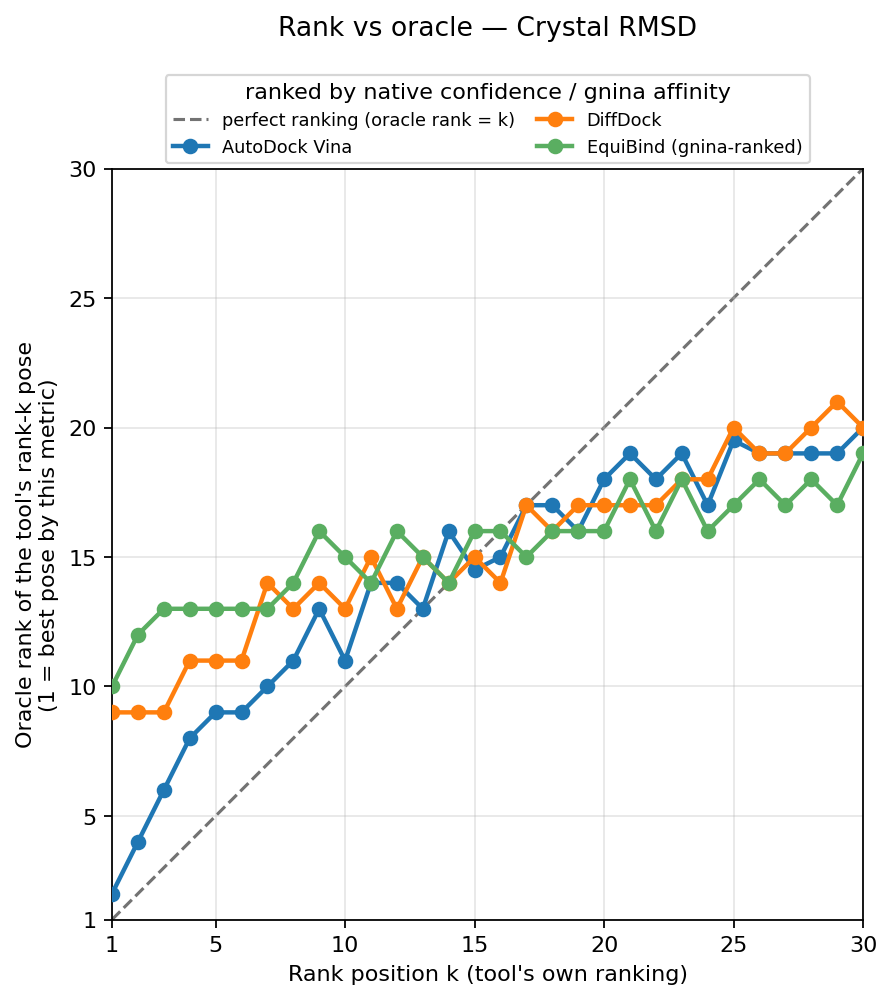
\includegraphics[width=\linewidth,height=0.78\textheight,keepaspectratio]{media/media/image29.png}
\caption{Rank versus oracle for as-placed crystal RMSD. The horizontal axis is each tool's own rank position k and the vertical axis the median oracle rank of the pose it placed at k, where oracle rank 1 is the pose closest to the crystal ligand. The dashed diagonal is perfect ranking and 15.5 is the expected oracle rank under random ordering}\label{fig:appendix-r28a}
\end{figure}

By as-placed crystal RMSD, the criterion that rewards putting the ligand in the right place, AutoDock Vina is the only tool whose ordering carries appreciable signal. Its rank-1 pose is the second best of its roughly thirty, its rank-2 pose the fourth best and its rank-3 pose the sixth best, so its curve lies closest to the diagonal at early ranks before rising towards the mid-range around k \ensuremath{\approx} 15. DiffDock and EquiBind both start far above the diagonal, with their most confident pose landing only at median oracle rank 9 and 10 respectively, so their ordering is weak, although the distance from the mid-range value shows it is not entirely absent. A tool's single most trusted pose is therefore rarely its own best-placed pose, and the ranking signal that does exist is concentrated at the top of each list.

\begin{figure}[!htbp]
\centering
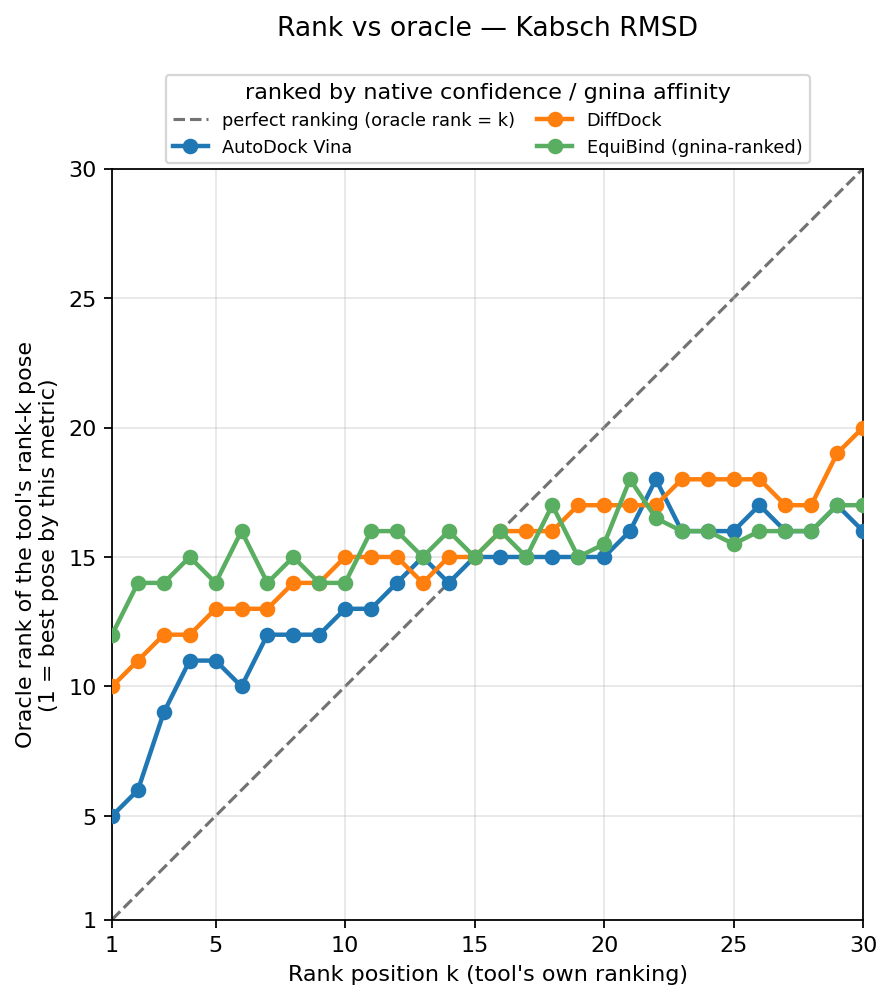
\includegraphics[width=\linewidth,height=0.78\textheight,keepaspectratio]{media/media/image30.png}
\caption{Rank versus oracle for best-fit (Kabsch) RMSD, representing internal form after optimal superposition. Axes as in Figure~\ref{fig:appendix-r28a}}\label{fig:appendix-r28b}
\end{figure}

Figure~\ref{fig:appendix-r28b} repeats the construction with best-fit Kabsch RMSD as the oracle criterion, which measures the residual conformational difference remaining after the pose is optimally superposed on the crystal ligand, that is its internal form with placement removed. Here every curve moves towards the mid-range and the advantage Vina held on placement disappears. Its rank-1 pose is now only the fifth best of its set by form, while DiffDock and EquiBind place their top pose at oracle rank 10 and 12 respectively. On form the physics-based and learned orderings are statistically indistinguishable, and DiffDock's median concordance is in fact nominally the higher of the two (\ensuremath{\tau} = 0.122 against Vina's 0.108, p = 0.504), while EquiBind's gnina order carries essentially no form signal (\ensuremath{\tau} = 0.048). No tool orders its own poses well by pure internal shape, which shows that the ranking signal Vina does possess concerns where the ligand sits rather than how its conformation is resolved.

\begin{figure}[!htbp]
\centering
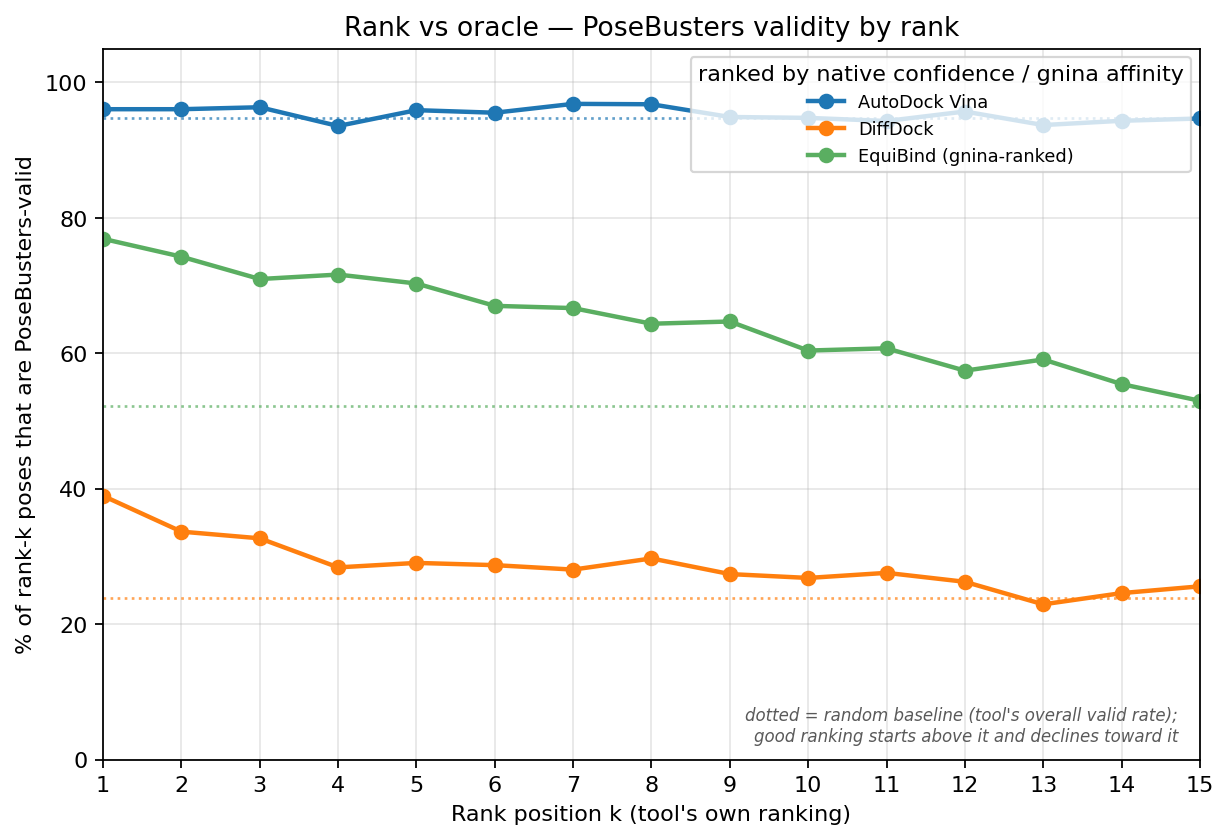
\includegraphics[width=\linewidth,height=0.78\textheight,keepaspectratio]{media/media/image31.png}
\caption{PoseBusters validity by rank. The solid curve is the percentage of rank-k poses that are PoseBusters-valid and the dotted line is each tool's overall valid rate, the random-order reference. Good ranking starts above the dotted line and declines towards it}\label{fig:appendix-r28c}
\end{figure}

Figure~\ref{fig:appendix-r28c} changes the question, because PoseBusters validity is binary and admits no oracle rank. Instead the panel plots, at each rank position, the percentage of rank-k poses that pass the PoseBusters checks, with each tool's overall valid rate drawn as a dotted random-order reference. A useful validity ranker starts above its dotted line and decays towards it as rank worsens. AutoDock Vina is essentially flat at about 94 to 97\% across all ranks, sitting on its own high baseline because nearly every Vina pose is already valid and there is little left to sort. DiffDock front-loads validity in the right direction but from a low level, falling from about 39\% at rank 1 to its 24\% baseline, so that even its most confident pose is more likely invalid than valid. The gnina-optimised, gnina-ranked EquiBind variant shows the clearest ranking signal on the plot, declining broadly, if not strictly monotonically, from about 77\% at rank 1 towards its 52\% baseline, which makes gnina affinity an effective validity sorter for these EquiBind poses even though it is a weak geometry sorter.

\begin{figure}[!htbp]
\centering
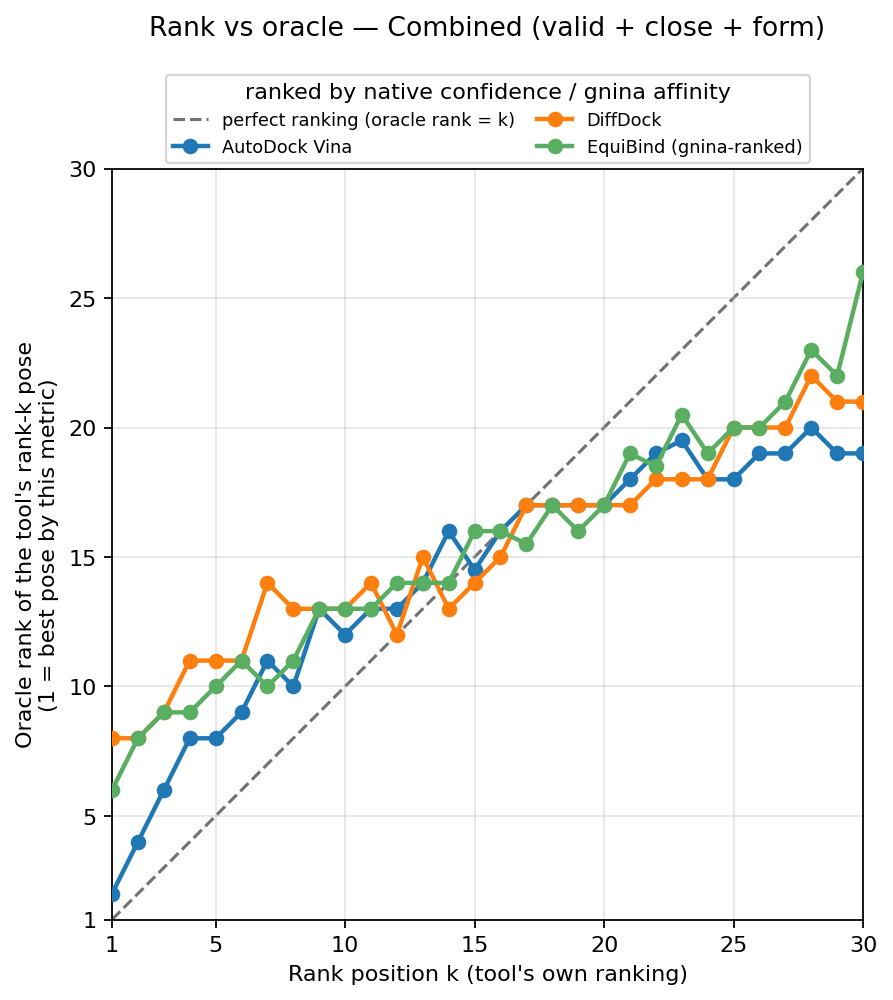
\includegraphics[width=\linewidth,height=0.78\textheight,keepaspectratio]{media/media/image32.png}
\caption{Rank versus oracle for the combined deployment criterion (validity, then placement, then form). PoseBusters-invalid poses are penalised below valid poses before valid poses are ordered by geometry. Axes as in Figure~\ref{fig:appendix-r28a}}\label{fig:appendix-r28d}
\end{figure}

Figure~\ref{fig:appendix-r28d} applies a deployment-relevant oracle criterion, in which a global penalty forces every PoseBusters-invalid pose below every valid one within a complex and the surviving valid poses are then ordered by placement and form together. It is an evaluation target rather than a selector usable in practice, since it relies on crystal RMSD, which is unavailable at real deployment time. The composite is also structurally opinionated, prioritising validity lexicographically and then summing crystal and Kabsch RMSD with equal weight, so that form is partly double-counted because as-placed RMSD already contains conformational error, and every conclusion drawn from the panel is conditional on that prespecified choice. Vina's rank-1 pose sits at oracle rank 2, almost unchanged from its crystal curve because it is already about 95\% valid and the validity-first key barely reshuffles it. DiffDock improves slightly to oracle rank 8, helped by the validity front-loading. The clearest movement is EquiBind, whose rank-1 pose rises to oracle rank 6, better than its crystal figure of 10 or Kabsch figure of 12 and now ahead of DiffDock. Because the composite rewards validity first, EquiBind's strong validity ordering lifts its whole-list concordance to a level not detectably different from Vina's, although Vina retains the better descriptive rank-1 median.

The four line charts are deliberately free of inference marks, so the formal comparison rests on three layers of distribution-free statistics computed per complex. First, a Kendall \ensuremath{\tau}-b correlation between each tool's rank order and the oracle badness order reduces every complex to a single concordance score, where +1 is perfect agreement, 0 is chance and \ensuremath{-}1 is a reversed ordering. A complex contributes only when it has at least three poses with non-constant rank and badness, which is why the validity \ensuremath{\tau} is defined solely on the mixed-validity complexes that contain both valid and invalid poses, namely 94 for Vina, 237 for DiffDock and 213 for EquiBind. The resulting per-tool medians are collected in Table~\ref{tab:appendix-ranking-concordance}.

\begin{longtable}[]{@{}
  >{\raggedright\arraybackslash}p{(\columnwidth - 6\tabcolsep) * \real{0.2500}}
  >{\raggedright\arraybackslash}p{(\columnwidth - 6\tabcolsep) * \real{0.2500}}
  >{\raggedright\arraybackslash}p{(\columnwidth - 6\tabcolsep) * \real{0.2500}}
  >{\raggedright\arraybackslash}p{(\columnwidth - 6\tabcolsep) * \real{0.2500}}@{}}
\caption{Median Per-Complex Kendall Tau-b between Tool Ranking and Oracle Badness}\tabularnewline
\toprule\noalign{}
{\raggedright Criterion} & {\raggedright AutoDock Vina} & {\raggedright DiffDock} & {\raggedright EquiBind (gnina-ranked)} \\
\midrule\noalign{}
\endfirsthead
\caption[]{Median Per-Complex Kendall Tau-b between Tool Ranking and Oracle Badness (continued)}\tabularnewline
\toprule\noalign{}
{\raggedright Criterion} & {\raggedright AutoDock Vina} & {\raggedright DiffDock} & {\raggedright EquiBind (gnina-ranked)} \\
\midrule\noalign{}
\endhead
\bottomrule\noalign{}
\endlastfoot
Crystal RMSD (placement) & 0.271 & 0.154 & 0.140 \\
Kabsch RMSD (form) & 0.108 & 0.122 & 0.048 \\
PoseBusters validity & 0.064 & 0.176 & 0.467 \\
Combined (valid + close + form) & 0.273 & 0.209 & 0.333 \\
\end{longtable}
\labelcurrenttable{tab:appendix-ranking-concordance}

A Friedman omnibus with Kendall's W as its effect size then asks whether the three tools' per-complex \ensuremath{\tau} differ, and a Wilcoxon signed-rank test with Holm correction and a matched-pairs rank-biserial effect size resolves the individual pairs. Every omnibus is highly significant (p \textless{} 0.0001), but the large sample simply confers high power, and it is Kendall's W that measures how large the systematic between-tool effect actually is. For the geometric criteria Kendall's W is only 0.050 for crystal, 0.035 for Kabsch and 0.034 for the combined score, which indicates a small between-tool effect against considerable complex-to-complex variation, so the population ordering does not translate into a reliable per-complex ranking. Only physical validity produces a substantial and stable ordering, with W = 0.341, and even that rests on just the 43 complexes that are mixed-validity for all three tools at once. On the pairwise tests Vina beats DiffDock and DiffDock beats EquiBind on crystal RMSD (rank-biserial +0.25 and +0.24, with Vina over EquiBind at +0.44), Vina and DiffDock tie on Kabsch while both beat EquiBind, EquiBind dominates both on validity (rank-biserial \ensuremath{-}0.80 against Vina and \ensuremath{-}0.89 against DiffDock), and on the combined criterion Vina beats DiffDock (p = 0.001) and EquiBind beats DiffDock (p = 0.004) while Vina and EquiBind show no significant difference (p = 0.496), which is an absence of a detected difference rather than demonstrated equivalence. One further caution applies to the tails of the curves, where the number of contributing complexes falls unequally across tools, from 303 at rank 1 to 149 for Vina, 285 for DiffDock and 302 for EquiBind at rank 30, so deep-rank comparisons rest on different subsets and are read only qualitatively. The persistence of signal into the tail is nonetheless visible, for example in EquiBind's combined median of 26 at rank 30, which shows its lowest-ranked poses being pushed towards the bottom of the pool.

Three findings follow, each requiring careful framing. AutoDock Vina is the strongest self-ranker for placement in this diagnostic, but the effect is a population tendency rather than a per-complex guarantee. Its use of the same empirical function during search and final ordering is a plausible mechanism for self-consistency \cite{ref022}, \cite{ref052}, but that mechanism is not directly tested here.

Second, both learned ranking pipelines retain a large selection gap. DiffDock\textquotesingle s native confidence and EquiBind\textquotesingle s gnina re-ranking place their top pose only around the ninth or tenth best of thirty by crystal placement, better than chance but far from the oracle. This is consistent with reported confidence-calibration and generalisation limitations for early learned docking systems \cite{ref024}, \cite{ref035}. Third, internal form is difficult for every score. All three rank Kabsch form less effectively than placement, and gnina ranking carries little form signal for EquiBind.

The single largest number in the analysis, gnina-ranked EquiBind's validity \ensuremath{\tau} of 0.467, is genuine but must not be read as evidence that EquiBind is intrinsically the better-ranking tool, because it is confounded in three ways. The validity \ensuremath{\tau} is defined only on mixed-validity complexes, and EquiBind, valid barely half the time overall, contributes 213 such information-rich complexes whereas Vina, valid about 95\% of the time, contributes only 94, and those 94 are Vina's hardest cases, so the three tools are scored on non-comparable subpopulations with only 43 in common. The ranker doing the work is gnina, a convolutional network trained to recognise realistic protein--ligand geometry, so its validity enrichment is an empirical property rather than something it was explicitly trained for, and the result largely restates that a geometry-aware model orders validity better than scores never aimed at it. And because the gnina poses are energy-minimised, gnina both optimises and ranks the EquiBind poses, so this is not a clean rescoring-only comparison nor a measurement of intrinsic EquiBind behaviour. The honest reading is that a validity-aware rescorer recovers usable ordering from a model that emits none, not that EquiBind holds an intrinsic ranking advantage, and this is single-model rescoring rather than any consensus effect.

The combined-criterion result for Vina and EquiBind is likewise structural rather than evidence of equivalence. The validity-first composite favours the gnina-ranked EquiBind subset because gnina both optimises and orders those poses, while Vina remains descriptively stronger at rank 1. The appropriate conclusion is limited to this diagnostic, namely that gnina can enrich valid EquiBind poses within mixed-validity complexes, but that does not overcome EquiBind\textquotesingle s low absolute near-native recovery or establish prospective parity with Vina.

Together, these panels illustrate the established separation between sampling and scoring \cite{ref050}, \cite{ref052}. The main recovery curves show that acceptable poses are sometimes present below rank 1, while the oracle-rank curves show that the tested scores do not reliably surface them. Vina retains the strongest placement ordering, raw learned output exhibits the physical-validity failures emphasised by PoseBusters \cite{ref035}, and gnina demonstrates that an external learned score can recover some useful ordering \cite{ref067}. Every continuous ranking result remains a population tendency, and the EquiBind validity result describes gnina\textquotesingle s behaviour on a favourable mixed-validity subset rather than an intrinsic EquiBind capability.

Tables~\ref{tab:appendix-oracle-ranks} and \ref{tab:appendix-validity-by-rank} provide the numerical data for Figure R28. Table~\ref{tab:appendix-oracle-ranks} lists median oracle rank for the crystal, Kabsch and combined criteria of Figures~\ref{fig:appendix-r28a}, \ref{fig:appendix-r28b} and \ref{fig:appendix-r28d}. Table~\ref{tab:appendix-validity-by-rank} lists PoseBusters validity by rank for Figure~\ref{fig:appendix-r28c}.

\begin{landscape}
\scriptsize
\setlength{\tabcolsep}{2pt}
\begin{longtable}[]{@{}
  >{\raggedright\arraybackslash}p{(\columnwidth - 18\tabcolsep) * \real{0.0992}}
  >{\raggedright\arraybackslash}p{(\columnwidth - 18\tabcolsep) * \real{0.0989}}
  >{\raggedright\arraybackslash}p{(\columnwidth - 18\tabcolsep) * \real{0.0999}}
  >{\raggedright\arraybackslash}p{(\columnwidth - 18\tabcolsep) * \real{0.1015}}
  >{\raggedright\arraybackslash}p{(\columnwidth - 18\tabcolsep) * \real{0.0989}}
  >{\raggedright\arraybackslash}p{(\columnwidth - 18\tabcolsep) * \real{0.0999}}
  >{\raggedright\arraybackslash}p{(\columnwidth - 18\tabcolsep) * \real{0.1015}}
  >{\raggedright\arraybackslash}p{(\columnwidth - 18\tabcolsep) * \real{0.0989}}
  >{\raggedright\arraybackslash}p{(\columnwidth - 18\tabcolsep) * \real{0.1000}}
  >{\raggedright\arraybackslash}p{(\columnwidth - 18\tabcolsep) * \real{0.1015}}@{}}
\caption{Median Oracle Rank at Positions 1--15}\tabularnewline
\toprule\noalign{}
{\raggedright \protect\hypertarget{_Toc235735959}{}{}\textbf{Rank k}} & {\raggedright \protect\hypertarget{_Toc235735960}{}{}\textbf{Vina (C)}} & {\raggedright \protect\hypertarget{_Toc235735961}{}{}\textbf{DiffDock (C)}} & {\raggedright \protect\hypertarget{_Toc235735962}{}{}\textbf{EquiBind (C)}} & {\raggedright \protect\hypertarget{_Toc235735963}{}{}\textbf{Vina (K)}} & {\raggedright \protect\hypertarget{_Toc235735964}{}{}\textbf{DiffDock (K)}} & {\raggedright \protect\hypertarget{_Toc235735965}{}{}\textbf{EquiBind (K)}} & {\raggedright \protect\hypertarget{_Toc235735966}{}{}\textbf{Vina (Cb)}} & {\raggedright \protect\hypertarget{_Toc235735967}{}{}\textbf{DiffDock (Cb)}} & {\raggedright \protect\hypertarget{_Toc235735968}{}{}\textbf{EquiBind (Cb)}} \\
\midrule\noalign{}
\endfirsthead
\caption[]{Median Oracle Rank at Positions 1--15 (continued)}\tabularnewline
\toprule\noalign{}
{\raggedright \protect\hypertarget{_Toc235735959}{}{}\textbf{Rank k}} & {\raggedright \protect\hypertarget{_Toc235735960}{}{}\textbf{Vina (C)}} & {\raggedright \protect\hypertarget{_Toc235735961}{}{}\textbf{DiffDock (C)}} & {\raggedright \protect\hypertarget{_Toc235735962}{}{}\textbf{EquiBind (C)}} & {\raggedright \protect\hypertarget{_Toc235735963}{}{}\textbf{Vina (K)}} & {\raggedright \protect\hypertarget{_Toc235735964}{}{}\textbf{DiffDock (K)}} & {\raggedright \protect\hypertarget{_Toc235735965}{}{}\textbf{EquiBind (K)}} & {\raggedright \protect\hypertarget{_Toc235735966}{}{}\textbf{Vina (Cb)}} & {\raggedright \protect\hypertarget{_Toc235735967}{}{}\textbf{DiffDock (Cb)}} & {\raggedright \protect\hypertarget{_Toc235735968}{}{}\textbf{EquiBind (Cb)}} \\
\midrule\noalign{}
\endhead
\bottomrule\noalign{}
\endlastfoot
\protect\hypertarget{_Toc235735969}{}{}1 & \protect\hypertarget{_Toc235735970}{}{}2 & \protect\hypertarget{_Toc235735971}{}{}9 & \protect\hypertarget{_Toc235735972}{}{}10 & \protect\hypertarget{_Toc235735973}{}{}5 & \protect\hypertarget{_Toc235735974}{}{}10 & \protect\hypertarget{_Toc235735975}{}{}12 & \protect\hypertarget{_Toc235735976}{}{}2 & \protect\hypertarget{_Toc235735977}{}{}8 & \protect\hypertarget{_Toc235735978}{}{}6 \\
\protect\hypertarget{_Toc235735979}{}{}2 & \protect\hypertarget{_Toc235735980}{}{}4 & \protect\hypertarget{_Toc235735981}{}{}9 & \protect\hypertarget{_Toc235735982}{}{}12 & \protect\hypertarget{_Toc235735983}{}{}6 & \protect\hypertarget{_Toc235735984}{}{}11 & \protect\hypertarget{_Toc235735985}{}{}14 & \protect\hypertarget{_Toc235735986}{}{}4 & \protect\hypertarget{_Toc235735987}{}{}8 & \protect\hypertarget{_Toc235735988}{}{}8 \\
\protect\hypertarget{_Toc235735989}{}{}3 & \protect\hypertarget{_Toc235735990}{}{}6 & \protect\hypertarget{_Toc235735991}{}{}9 & \protect\hypertarget{_Toc235735992}{}{}13 & \protect\hypertarget{_Toc235735993}{}{}9 & \protect\hypertarget{_Toc235735994}{}{}12 & \protect\hypertarget{_Toc235735995}{}{}14 & \protect\hypertarget{_Toc235735996}{}{}6 & \protect\hypertarget{_Toc235735997}{}{}9 & \protect\hypertarget{_Toc235735998}{}{}9 \\
\protect\hypertarget{_Toc235735999}{}{}4 & \protect\hypertarget{_Toc235736000}{}{}8 & \protect\hypertarget{_Toc235736001}{}{}11 & \protect\hypertarget{_Toc235736002}{}{}13 & \protect\hypertarget{_Toc235736003}{}{}11 & \protect\hypertarget{_Toc235736004}{}{}12 & \protect\hypertarget{_Toc235736005}{}{}15 & \protect\hypertarget{_Toc235736006}{}{}8 & \protect\hypertarget{_Toc235736007}{}{}11 & \protect\hypertarget{_Toc235736008}{}{}9 \\
\protect\hypertarget{_Toc235736009}{}{}5 & \protect\hypertarget{_Toc235736010}{}{}9 & \protect\hypertarget{_Toc235736011}{}{}11 & \protect\hypertarget{_Toc235736012}{}{}13 & \protect\hypertarget{_Toc235736013}{}{}11 & \protect\hypertarget{_Toc235736014}{}{}13 & \protect\hypertarget{_Toc235736015}{}{}14 & \protect\hypertarget{_Toc235736016}{}{}8 & \protect\hypertarget{_Toc235736017}{}{}11 & \protect\hypertarget{_Toc235736018}{}{}10 \\
\protect\hypertarget{_Toc235736019}{}{}6 & \protect\hypertarget{_Toc235736020}{}{}9 & \protect\hypertarget{_Toc235736021}{}{}11 & \protect\hypertarget{_Toc235736022}{}{}13 & \protect\hypertarget{_Toc235736023}{}{}10 & \protect\hypertarget{_Toc235736024}{}{}13 & \protect\hypertarget{_Toc235736025}{}{}16 & \protect\hypertarget{_Toc235736026}{}{}9 & \protect\hypertarget{_Toc235736027}{}{}11 & \protect\hypertarget{_Toc235736028}{}{}11 \\
\protect\hypertarget{_Toc235736029}{}{}7 & \protect\hypertarget{_Toc235736030}{}{}10 & \protect\hypertarget{_Toc235736031}{}{}14 & \protect\hypertarget{_Toc235736032}{}{}13 & \protect\hypertarget{_Toc235736033}{}{}12 & \protect\hypertarget{_Toc235736034}{}{}13 & \protect\hypertarget{_Toc235736035}{}{}14 & \protect\hypertarget{_Toc235736036}{}{}11 & \protect\hypertarget{_Toc235736037}{}{}14 & \protect\hypertarget{_Toc235736038}{}{}10 \\
\protect\hypertarget{_Toc235736039}{}{}8 & \protect\hypertarget{_Toc235736040}{}{}11 & \protect\hypertarget{_Toc235736041}{}{}13 & \protect\hypertarget{_Toc235736042}{}{}14 & \protect\hypertarget{_Toc235736043}{}{}12 & \protect\hypertarget{_Toc235736044}{}{}14 & \protect\hypertarget{_Toc235736045}{}{}15 & \protect\hypertarget{_Toc235736046}{}{}10 & \protect\hypertarget{_Toc235736047}{}{}13 & \protect\hypertarget{_Toc235736048}{}{}11 \\
\protect\hypertarget{_Toc235736049}{}{}9 & \protect\hypertarget{_Toc235736050}{}{}13 & \protect\hypertarget{_Toc235736051}{}{}14 & \protect\hypertarget{_Toc235736052}{}{}16 & \protect\hypertarget{_Toc235736053}{}{}12 & \protect\hypertarget{_Toc235736054}{}{}14 & \protect\hypertarget{_Toc235736055}{}{}14 & \protect\hypertarget{_Toc235736056}{}{}13 & \protect\hypertarget{_Toc235736057}{}{}13 & \protect\hypertarget{_Toc235736058}{}{}13 \\
\protect\hypertarget{_Toc235736059}{}{}10 & \protect\hypertarget{_Toc235736060}{}{}11 & \protect\hypertarget{_Toc235736061}{}{}13 & \protect\hypertarget{_Toc235736062}{}{}15 & \protect\hypertarget{_Toc235736063}{}{}13 & \protect\hypertarget{_Toc235736064}{}{}15 & \protect\hypertarget{_Toc235736065}{}{}14 & \protect\hypertarget{_Toc235736066}{}{}12 & \protect\hypertarget{_Toc235736067}{}{}13 & \protect\hypertarget{_Toc235736068}{}{}13 \\
\protect\hypertarget{_Toc235736069}{}{}11 & \protect\hypertarget{_Toc235736070}{}{}14 & \protect\hypertarget{_Toc235736071}{}{}15 & \protect\hypertarget{_Toc235736072}{}{}14 & \protect\hypertarget{_Toc235736073}{}{}13 & \protect\hypertarget{_Toc235736074}{}{}15 & \protect\hypertarget{_Toc235736075}{}{}16 & \protect\hypertarget{_Toc235736076}{}{}13 & \protect\hypertarget{_Toc235736077}{}{}14 & \protect\hypertarget{_Toc235736078}{}{}13 \\
\protect\hypertarget{_Toc235736079}{}{}12 & \protect\hypertarget{_Toc235736080}{}{}14 & \protect\hypertarget{_Toc235736081}{}{}13 & \protect\hypertarget{_Toc235736082}{}{}16 & \protect\hypertarget{_Toc235736083}{}{}14 & \protect\hypertarget{_Toc235736084}{}{}15 & \protect\hypertarget{_Toc235736085}{}{}16 & \protect\hypertarget{_Toc235736086}{}{}13 & \protect\hypertarget{_Toc235736087}{}{}12 & \protect\hypertarget{_Toc235736088}{}{}14 \\
\protect\hypertarget{_Toc235736089}{}{}13 & \protect\hypertarget{_Toc235736090}{}{}13 & \protect\hypertarget{_Toc235736091}{}{}15 & \protect\hypertarget{_Toc235736092}{}{}15 & \protect\hypertarget{_Toc235736093}{}{}15 & \protect\hypertarget{_Toc235736094}{}{}14 & \protect\hypertarget{_Toc235736095}{}{}15 & \protect\hypertarget{_Toc235736096}{}{}14 & \protect\hypertarget{_Toc235736097}{}{}15 & \protect\hypertarget{_Toc235736098}{}{}14 \\
\protect\hypertarget{_Toc235736099}{}{}14 & \protect\hypertarget{_Toc235736100}{}{}16 & \protect\hypertarget{_Toc235736101}{}{}14 & \protect\hypertarget{_Toc235736102}{}{}14 & \protect\hypertarget{_Toc235736103}{}{}14 & \protect\hypertarget{_Toc235736104}{}{}15 & \protect\hypertarget{_Toc235736105}{}{}16 & \protect\hypertarget{_Toc235736106}{}{}16 & \protect\hypertarget{_Toc235736107}{}{}13 & \protect\hypertarget{_Toc235736108}{}{}14 \\
\protect\hypertarget{_Toc235736109}{}{}15 & \protect\hypertarget{_Toc235736110}{}{}14 & \protect\hypertarget{_Toc235736111}{}{}15 & \protect\hypertarget{_Toc235736112}{}{}16 & \protect\hypertarget{_Toc235736113}{}{}15 & \protect\hypertarget{_Toc235736114}{}{}15 & \protect\hypertarget{_Toc235736115}{}{}15 & \protect\hypertarget{_Toc235736116}{}{}14 & \protect\hypertarget{_Toc235736117}{}{}14 & \protect\hypertarget{_Toc235736118}{}{}16 \\
\end{longtable}
\labelcurrenttable{tab:appendix-oracle-ranks}
\end{landscape}

\begin{landscape}
\scriptsize
\setlength{\tabcolsep}{2pt}
\begin{longtable}[]{@{}
  >{\raggedright\arraybackslash}p{(\columnwidth - 6\tabcolsep) * \real{0.2500}}
  >{\raggedright\arraybackslash}p{(\columnwidth - 6\tabcolsep) * \real{0.2500}}
  >{\raggedright\arraybackslash}p{(\columnwidth - 6\tabcolsep) * \real{0.2500}}
  >{\raggedright\arraybackslash}p{(\columnwidth - 6\tabcolsep) * \real{0.2500}}@{}}
\caption{PoseBusters Validity by Rank}\tabularnewline
\toprule\noalign{}
{\raggedright \protect\hypertarget{_Toc235736119}{}{}\textbf{Rank k}} & {\raggedright \protect\hypertarget{_Toc235736120}{}{}\textbf{AutoDock Vina}} & {\raggedright \protect\hypertarget{_Toc235736121}{}{}\textbf{DiffDock}} & {\raggedright \protect\hypertarget{_Toc235736122}{}{}\textbf{EquiBind (gnina-ranked)}} \\
\midrule\noalign{}
\endfirsthead
\caption[]{PoseBusters Validity by Rank (continued)}\tabularnewline
\toprule\noalign{}
{\raggedright \protect\hypertarget{_Toc235736119}{}{}\textbf{Rank k}} & {\raggedright \protect\hypertarget{_Toc235736120}{}{}\textbf{AutoDock Vina}} & {\raggedright \protect\hypertarget{_Toc235736121}{}{}\textbf{DiffDock}} & {\raggedright \protect\hypertarget{_Toc235736122}{}{}\textbf{EquiBind (gnina-ranked)}} \\
\midrule\noalign{}
\endhead
\bottomrule\noalign{}
\endlastfoot
\protect\hypertarget{_Toc235736123}{}{}1 & \protect\hypertarget{_Toc235736124}{}{}96 & \protect\hypertarget{_Toc235736125}{}{}39 & \protect\hypertarget{_Toc235736126}{}{}77 \\
\protect\hypertarget{_Toc235736127}{}{}2 & \protect\hypertarget{_Toc235736128}{}{}96 & \protect\hypertarget{_Toc235736129}{}{}34 & \protect\hypertarget{_Toc235736130}{}{}74 \\
\protect\hypertarget{_Toc235736131}{}{}3 & \protect\hypertarget{_Toc235736132}{}{}96 & \protect\hypertarget{_Toc235736133}{}{}33 & \protect\hypertarget{_Toc235736134}{}{}71 \\
\protect\hypertarget{_Toc235736135}{}{}4 & \protect\hypertarget{_Toc235736136}{}{}94 & \protect\hypertarget{_Toc235736137}{}{}28 & \protect\hypertarget{_Toc235736138}{}{}72 \\
\protect\hypertarget{_Toc235736139}{}{}5 & \protect\hypertarget{_Toc235736140}{}{}96 & \protect\hypertarget{_Toc235736141}{}{}29 & \protect\hypertarget{_Toc235736142}{}{}70 \\
\protect\hypertarget{_Toc235736143}{}{}6 & \protect\hypertarget{_Toc235736144}{}{}96 & \protect\hypertarget{_Toc235736145}{}{}29 & \protect\hypertarget{_Toc235736146}{}{}67 \\
\protect\hypertarget{_Toc235736147}{}{}7 & \protect\hypertarget{_Toc235736148}{}{}97 & \protect\hypertarget{_Toc235736149}{}{}28 & \protect\hypertarget{_Toc235736150}{}{}67 \\
\protect\hypertarget{_Toc235736151}{}{}8 & \protect\hypertarget{_Toc235736152}{}{}97 & \protect\hypertarget{_Toc235736153}{}{}30 & \protect\hypertarget{_Toc235736154}{}{}64 \\
\protect\hypertarget{_Toc235736155}{}{}9 & \protect\hypertarget{_Toc235736156}{}{}95 & \protect\hypertarget{_Toc235736157}{}{}27 & \protect\hypertarget{_Toc235736158}{}{}65 \\
\protect\hypertarget{_Toc235736159}{}{}10 & \protect\hypertarget{_Toc235736160}{}{}95 & \protect\hypertarget{_Toc235736161}{}{}27 & \protect\hypertarget{_Toc235736162}{}{}60 \\
\protect\hypertarget{_Toc235736163}{}{}11 & \protect\hypertarget{_Toc235736164}{}{}94 & \protect\hypertarget{_Toc235736165}{}{}28 & \protect\hypertarget{_Toc235736166}{}{}61 \\
\protect\hypertarget{_Toc235736167}{}{}12 & \protect\hypertarget{_Toc235736168}{}{}96 & \protect\hypertarget{_Toc235736169}{}{}26 & \protect\hypertarget{_Toc235736170}{}{}57 \\
\protect\hypertarget{_Toc235736171}{}{}13 & \protect\hypertarget{_Toc235736172}{}{}94 & \protect\hypertarget{_Toc235736173}{}{}23 & \protect\hypertarget{_Toc235736174}{}{}59 \\
\protect\hypertarget{_Toc235736175}{}{}14 & \protect\hypertarget{_Toc235736176}{}{}94 & \protect\hypertarget{_Toc235736177}{}{}25 & \protect\hypertarget{_Toc235736178}{}{}55 \\
\protect\hypertarget{_Toc235736179}{}{}15 & \protect\hypertarget{_Toc235736180}{}{}95 & \protect\hypertarget{_Toc235736181}{}{}26 & \protect\hypertarget{_Toc235736182}{}{}53 \\
\end{longtable}
\labelcurrenttable{tab:appendix-validity-by-rank}
\end{landscape}

\hypertarget{dataset}{%
\chapter{Dataset}\label{dataset}}

The PoseBusters benchmark provides 308 high-resolution protein-ligand crystal structures released after 2021 for testing generated poses \cite{ref035}. The release window reduces exact-entry overlap with the nominal training cutoff of early learned docking models, but it does not exclude related proteins, ligands, pockets or templates. The present study maps the chemical and structural breadth of the source set and compares it with the three Orai1-related docking inputs.

\hypertarget{composition-and-provenance}{%
\section{Composition and Provenance}\label{composition-and-provenance}}

Each of the 308 entries pairs one receptor with one cognate ligand, every complex carrying a distinct PDB identifier and a distinct ligand (308 unique PDB IDs and 308 unique chemical-component codes)\footnote{For every entry the benchmark provides four files, namely the receptor stripped of solvent but retaining its cofactors (*\_protein.pdb), all crystallographic instances of the ligand of interest (*\_ligands.sdf), the single chosen crystal instance that serves as the ground-truth answer pose (*\_ligand.sdf), and one computer-generated starting conformer produced with RDKit's ETKDGv3 algorithm followed by UFF minimisation (*\_ligand\_start\_conf.sdf).}. The crystallographic pose is the experimentally validated reference for scoring every docked pose, while the generated start conformer mimics the ligand information a docking engine sees at run time.

The experimentally resolved ligand conformations provide a reference for symmetry-corrected pose comparison. However, a later PDB release date is not proof that the biological or chemical pattern was absent from training data. Homology-, pocket-, scaffold- and template-similarity analyses are needed before making a strong no-leakage claim. Multiple crystallographic copies of the same ligand within a structure are handled by the stated symmetry-corrected comparison.

\hypertarget{ligand-physicochemical-profile}{%
\section{Ligand Physicochemical Profile}\label{ligand-physicochemical-profile}}

The 308 source ligands cover a wide region of chemical space. The median ligand has 24 heavy atoms, with an interquartile range of 16 to 32 and a full range of 6 to 64, and a median molecular weight of 359 Da. The distributions are right-skewed and extend beyond 600 Da, reflecting peptides, nucleotides, sugars and cofactor-like molecules alongside conventional small molecules (Figure~\ref{fig:appendix-dataset-1}). The median ligand has five rotatable bonds, six hydrogen-bond acceptors, three donors and a topological polar surface area of 107 \angstrom{}\textsuperscript{2}.

\begin{figure}[!htbp]
\centering

\includegraphics[width=\linewidth,height=0.78\textheight,keepaspectratio]{media/media/image33.png}
\caption{Univariate distributions of twelve physicochemical attributes across the 308 benchmark ligands}\label{fig:appendix-dataset-1}
\end{figure}

\begin{longtable}[]{@{}
  >{\raggedright\arraybackslash}p{(\columnwidth - 6\tabcolsep) * \real{0.3528}}
  >{\raggedright\arraybackslash}p{(\columnwidth - 6\tabcolsep) * \real{0.1472}}
  >{\raggedright\arraybackslash}p{(\columnwidth - 6\tabcolsep) * \real{0.2500}}
  >{\raggedright\arraybackslash}p{(\columnwidth - 6\tabcolsep) * \real{0.2500}}@{}}
\caption{Distribution of Principal Ligand Descriptors in the PoseBusters Subset}\tabularnewline
\toprule\noalign{}
{\raggedright \textbf{Descriptor}} & {\raggedright \textbf{Median}} & {\raggedright \textbf{IQR (25--75\,\%)}} & {\raggedright \textbf{Range (min--max)}} \\
\midrule\noalign{}
\endfirsthead
\caption[]{Distribution of Principal Ligand Descriptors in the PoseBusters Subset (continued)}\tabularnewline
\toprule\noalign{}
{\raggedright \textbf{Descriptor}} & {\raggedright \textbf{Median}} & {\raggedright \textbf{IQR (25--75\,\%)}} & {\raggedright \textbf{Range (min--max)}} \\
\midrule\noalign{}
\endhead
\bottomrule\noalign{}
\endlastfoot
Heavy atoms & 24 & 16--32 & 6--64 \\
Molecular weight (Da) & 359 & 236--462 & 100--872 \\
Rotatable bonds & 5 & 2--7 & 0--20 \\
H-bond acceptors & 6 & 3--9 & 0--21 \\
H-bond donors & 3 & 2--5 & 0--13 \\
TPSA (\angstrom{}\textsuperscript{2}) & 107 & 66--160 & 0--384 \\
cLogP & 0.9 & \ensuremath{-}1.6--3.2 & \ensuremath{-}8.4--14.0 \\
Fraction sp\textsuperscript{3} C & 0.41 & 0.23--0.57 & 0.00--1.00 \\
QED & 0.44 & 0.29--0.60 & 0.04--0.91 \\
Ring count & 3 & 1--4 & 0--8 \\
\end{longtable}
\labelcurrenttable{tab:appendix-ligand-distribution}

\hypertarget{drug-likeness}{%
\section{Drug-Likeness}\label{drug-likeness}}

Drug-likeness metrics confirm that the set deliberately reaches past classical small-molecule drug space. Under Lipinski's rule of five,\footnote{Lipinski's ``rule of five'' is a heuristic for oral drug-likeness. Poor absorption or permeation is more likely when a compound has more than five hydrogen-bond donors, more than ten hydrogen-bond acceptors, a molecular weight above 500 Da, or a calculated logP (cLogP) above 5, each threshold being a multiple of five. See C. A. Lipinski, F. Lombardo, B. W. Dominy and P. J. Feeney, ``Experimental and computational approaches to estimate solubility and permeability in drug discovery and development settings'', Advanced Drug Delivery Reviews, 1997, 23 (1--3), 3--25 (DOI: 10.1016/S0169-409X(96)00423-1).} 83\% of ligands incur at most one violation and 65\% none at all, yet a substantial 17\% violate two or more criteria (Figure~\ref{fig:appendix-dataset-2}). The quantitative estimate of drug-likeness (QED) sits at a median of just 0.44, and only 67\% of ligands clear the 0.34 threshold usually called ``attractive''. This spread is intentional. Keeping polar, charged and oversized ligands stresses each method's ability to generalise rather than rewarding performance on an easy, lead-like subset.

\begin{figure}[!htbp]
\centering

\includegraphics[width=\linewidth,height=0.78\textheight,keepaspectratio]{media/media/image34.png}
\caption{Drug-likeness of the benchmark ligands. Lipinski rule-of-five violation counts (left), overall rule-of-five compliance (centre) and the QED distribution (right)}\label{fig:appendix-dataset-2}
\end{figure}

\hypertarget{elemental-and-charge-composition}{%
\section{Elemental and Charge Composition}\label{elemental-and-charge-composition}}

The elemental make-up widens the challenge further (Figure~\ref{fig:appendix-dataset-3}). Roughly a quarter of the ligands contain phosphorus (25\%) or sulfur (24\%), 22\% carry at least one halogen, and metal atoms are essentially absent from the ligand records. Net formal charges are uncommon, since only 3\% of ligands are charged and the vast majority are neutral, but the heteroatom count is high and broadly spread (median 8, reaching nearly 30), matching the many nucleotide- and phosphate-containing species. These are exactly the features that the physical and chemical validity checks, namely protonation, geometry and steric clashes, probe most sharply.

\begin{figure}[!htbp]
\centering
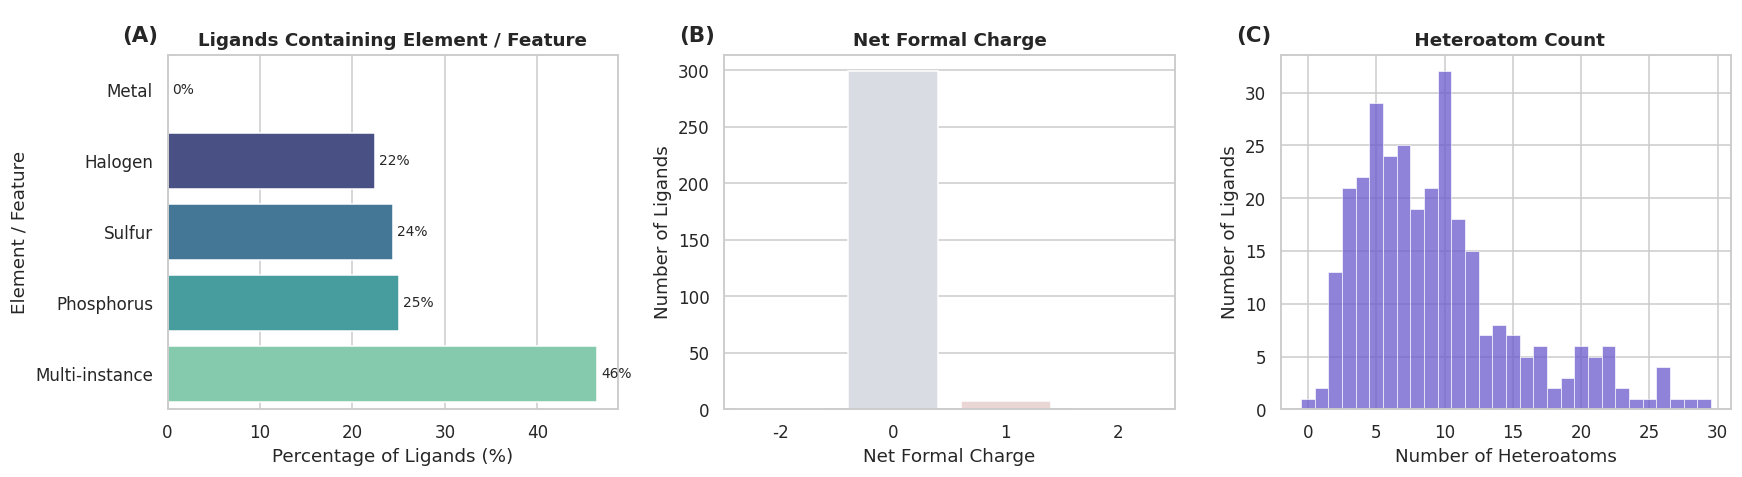
\includegraphics[width=\linewidth,height=0.78\textheight,keepaspectratio]{media/media/image35.png}
\caption{Elemental and charge composition. Prevalence of selected elements and features (left), formal-charge distribution (centre) and heteroatom counts (right)}\label{fig:appendix-dataset-3}
\end{figure}

\hypertarget{joint-distributions-and-correlation-structure}{%
\section{Joint Distributions and Correlation Structure}\label{joint-distributions-and-correlation-structure}}

The descriptors are considerably interdependent (Figure~\ref{fig:appendix-dataset-4}). The size-related quantities, namely heavy-atom count, molecular weight, hydrogen-bond acceptor count, polar surface area and heteroatom count, correlate strongly and positively, while QED falls as molecules grow larger and more polar. Lipophilicity runs opposite to polar surface area, and the sp\textsuperscript{3}-carbon fraction opposes aromatic-ring count, separating flat aromatic scaffolds from saturated three-dimensional ones. The two-dimensional mappings make this explicit. Heavy-atom and rotatable-bond counts rise together (r = +0.70) (Figure~\ref{fig:appendix-dataset-5}\,(A)), mass and polar surface area co-vary (r = +0.46), lipophilicity and polarity trade off (r = \ensuremath{-}0.61), and drug-likeness declines with size (r = \ensuremath{-}0.52) (Figure~\ref{fig:appendix-dataset-5}). The pairwise joint distributions of the six core descriptors (Figure~\ref{fig:appendix-dataset-6}) confirm that the benchmark forms one broad cloud rather than distinct clusters.

\begin{figure}[!htbp]
\centering
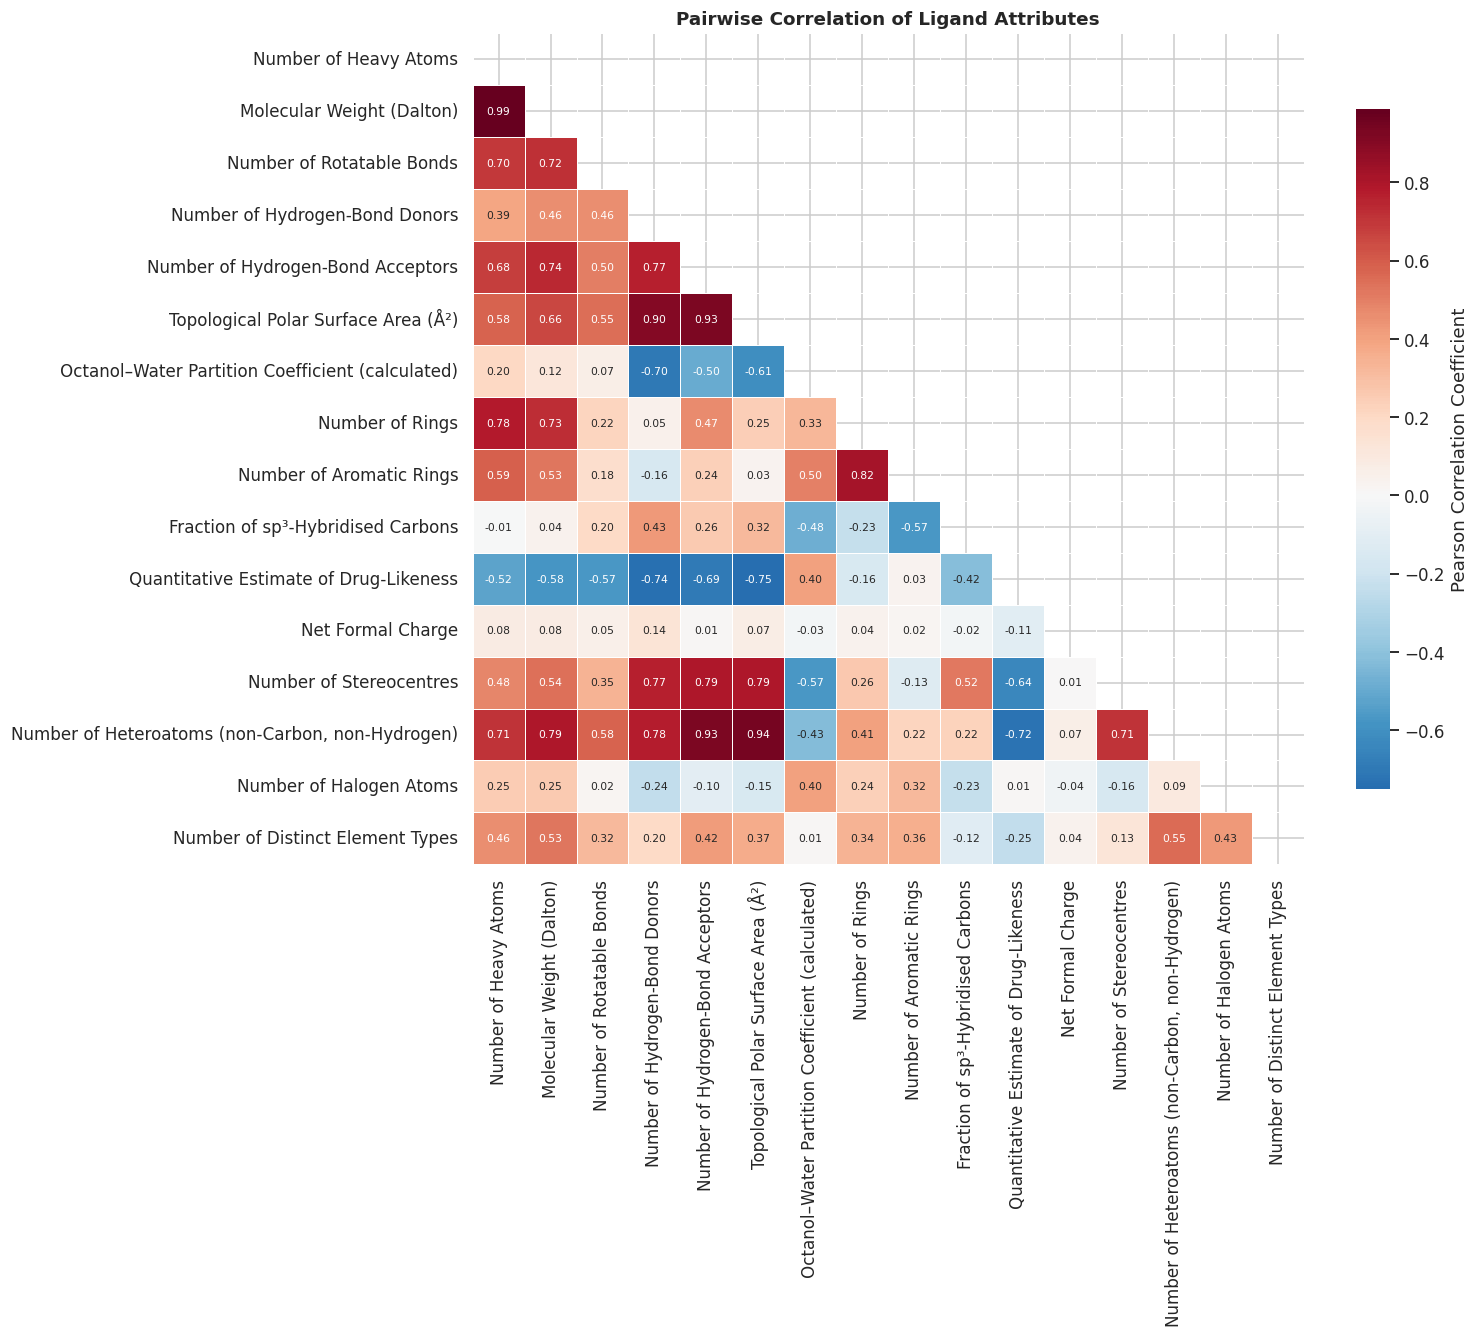
\includegraphics[width=\linewidth,height=0.78\textheight,keepaspectratio]{media/media/image36.png}
\caption{Pairwise Pearson correlation of the sixteen ligand descriptors}\label{fig:appendix-dataset-4}
\end{figure}

\begin{figure}[!htbp]
\centering

\includegraphics[width=\linewidth,height=0.78\textheight,keepaspectratio]{media/media/image37.png}
\caption{Two-dimensional attribute mappings with points coloured by QED. The JKU reference ligands are marked. R denotes the Pearson correlation}\label{fig:appendix-dataset-5}
\end{figure}

\begin{figure}[!htbp]
\centering
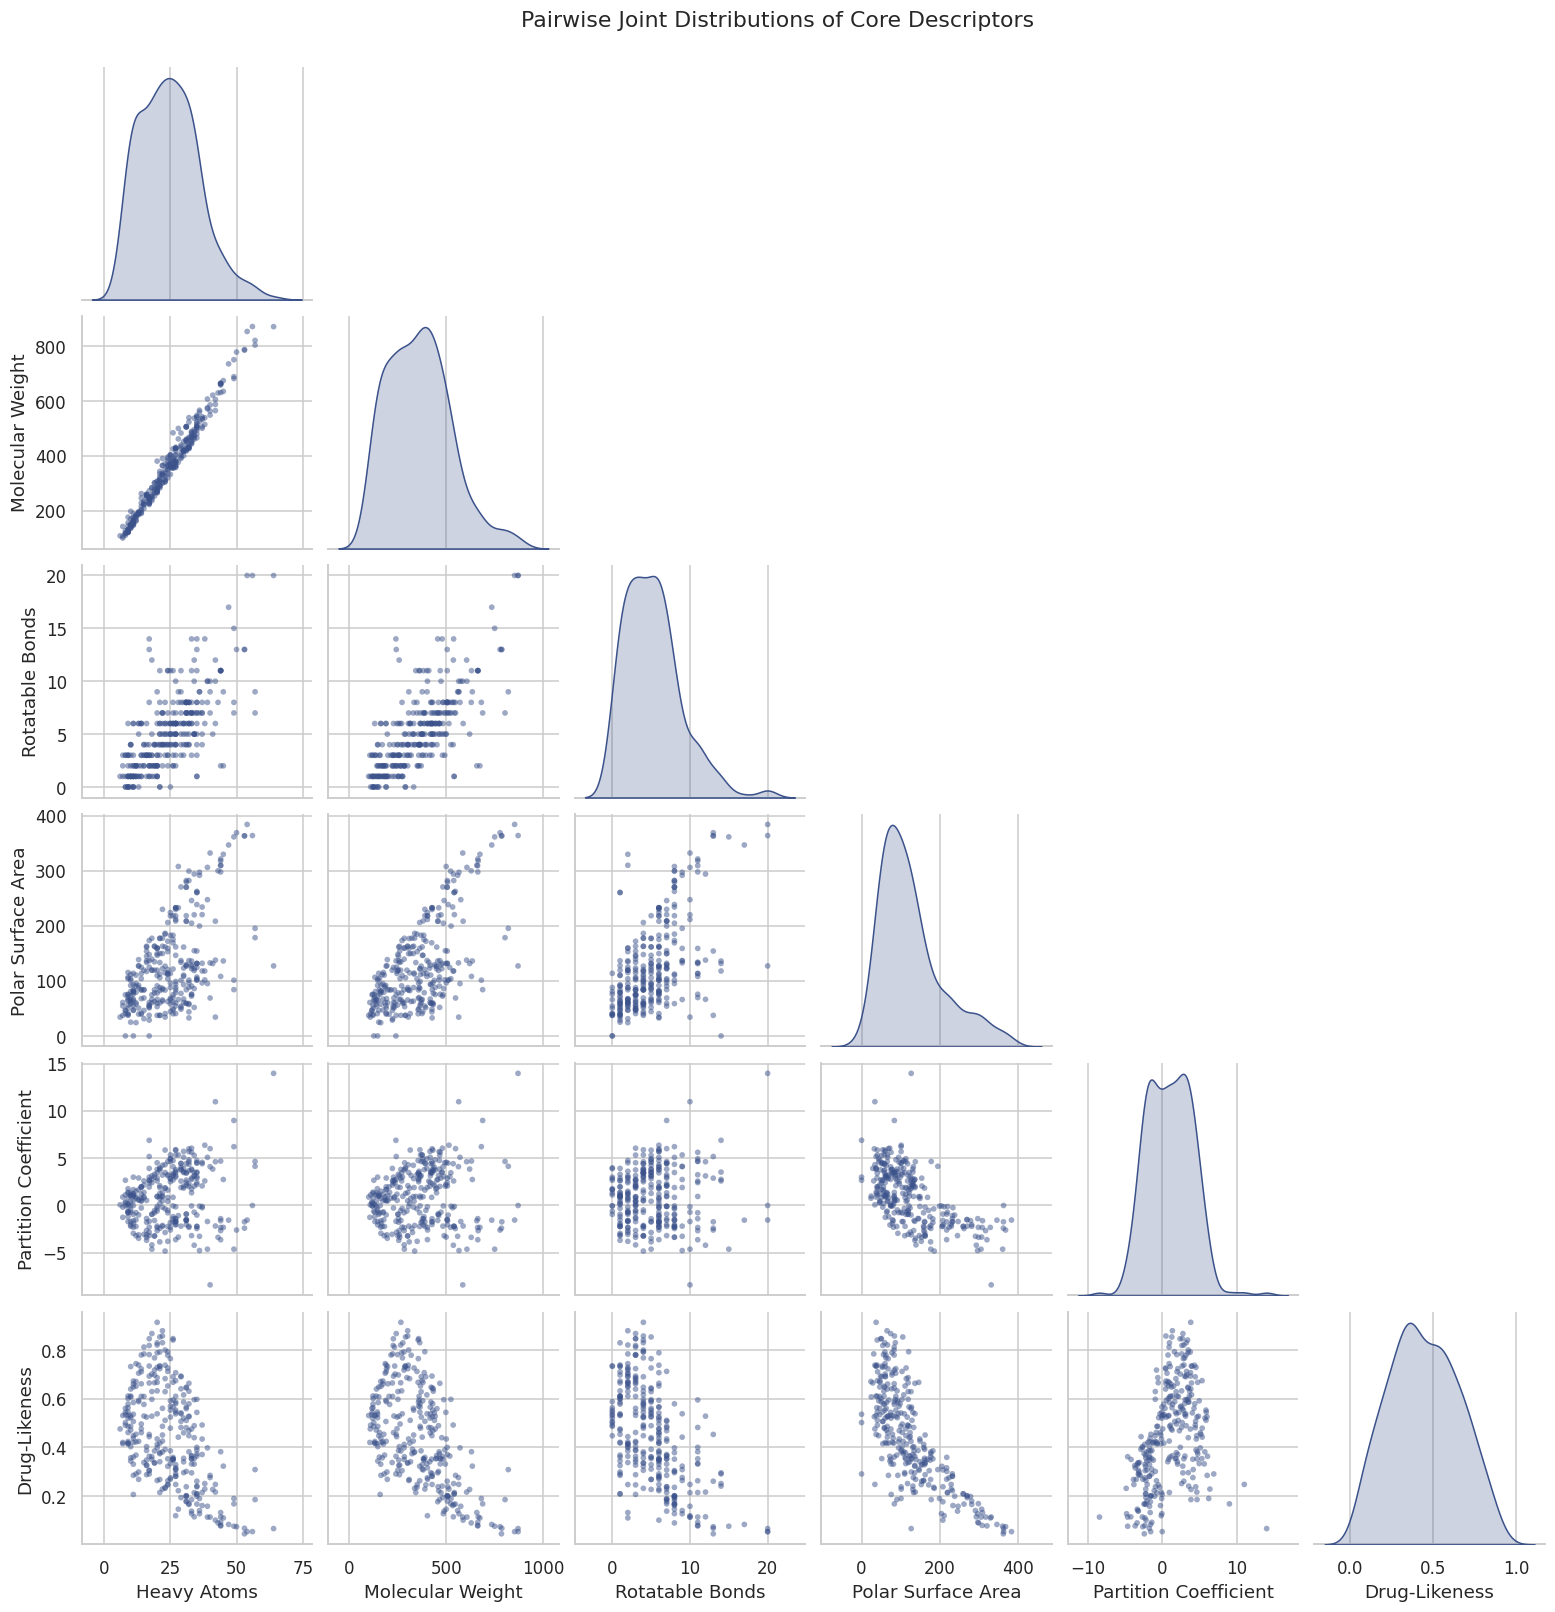
\includegraphics[width=\linewidth,height=0.78\textheight,keepaspectratio]{media/media/image38.png}
\caption{Pairwise joint distributions of six core descriptors with kernel-density estimates on the diagonal}\label{fig:appendix-dataset-6}
\end{figure}

\hypertarget{principal-component-analysis-chemical-space}{%
\section{Principal-Component Analysis --- Chemical Space}\label{principal-component-analysis-chemical-space}}

Summarising this correlated space, a principal-component analysis was run on the sixteen standardised ligand descriptors. Two components already capture roughly two-thirds of the variance (PC1 \ensuremath{\approx} 45\%, PC2 \ensuremath{\approx} 23\%) and four reach about 81\% (Figure~\ref{fig:appendix-dataset-7}), showing that only a few underlying factors govern the set's diversity. The first component is a size-and-polarity axis. Heavy-atom count, molecular weight, hydrogen-bond acceptors and donors, polar surface area, heteroatom and stereocentre counts all load strongly and positively, while QED loads strongly negative, so moving along PC1 trades rising size, polarity and complexity against falling drug-likeness. The second component separates flat, lipophilic, aromatic, halogenated scaffolds (positive loadings on aromatic rings, cLogP, ring count and halogen count) from saturated, sp\textsuperscript{3}-rich, hydrogen-bond-donating ones. The minor components capture halogenation and element diversity (PC3) and net formal charge (PC4). Overlaying the per-ligand difficulty of reproducing the crystal pose on the score plot, it rises towards positive PC1 (Figure~\ref{fig:appendix-dataset-8}), identifying molecular size and flexibility, not aromatic or lipophilic character, as the dominant driver of docking difficulty.

\begin{figure}[!htbp]
\centering
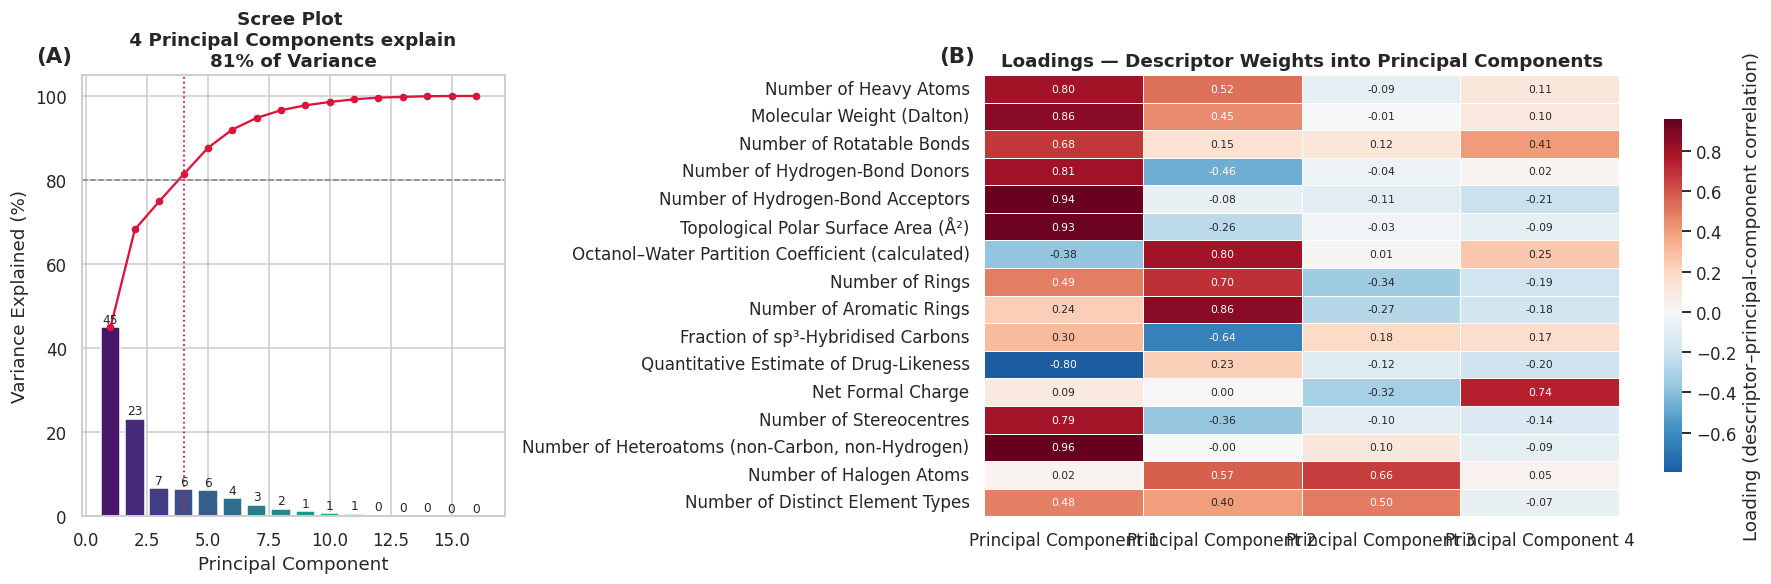
\includegraphics[width=\linewidth,height=0.78\textheight,keepaspectratio]{media/media/image39.png}
\caption{Principal-component analysis of the standardised ligand descriptors. Scree plot of explained variance (left) and component loadings (right)}\label{fig:appendix-dataset-7}
\end{figure}

\begin{figure}[!htbp]
\centering

\includegraphics[width=\linewidth,height=0.78\textheight,keepaspectratio]{media/media/image40.png}
\caption{PCA biplot with descriptor loadings (left) and PC scores coloured by conformer-generation difficulty (right). The experimentally validated ligands are projected into the same space}\label{fig:appendix-dataset-8}
\end{figure}

\hypertarget{receptor-profile}{%
\section{Receptor Profile}\label{receptor-profile}}

The receptor side is equally varied (Figure~\ref{fig:appendix-dataset-9}). A typical complex resolves 472 residues (interquartile range 306 to 778) and is a monomer or dimer, but the distribution has a long tail of large multi-chain assemblies running to forty chains and several thousand residues. Critically, 89\% of the complexes keep at least one cofactor or hetero-component, so the binding environments are realistic rather than artificially stripped. Ligand size is essentially independent of receptor size, meaning small ligands are docked into both small and very large pockets and receptor dimensions cannot act as a confounding shortcut.

\begin{figure}[!htbp]
\centering

\includegraphics[width=\linewidth,height=0.78\textheight,keepaspectratio]{media/media/image41.png}
\caption{Receptor profile. Resolved residues, chains per complex, distinct cofactor types and ligand-versus-receptor size}\label{fig:appendix-dataset-9}
\end{figure}

\hypertarget{conformer-generation-difficulty}{%
\section{Conformer-Generation Difficulty}\label{conformer-generation-difficulty}}

The single ETKDGv3+UFF starting conformer supplied with each ligand gives a lower-bound estimate of how far a docking engine must move the ligand to recover the crystal pose. The symmetry-corrected RMSD between this start conformer and the crystallographic pose has a median of 1.56\angstrom{}, and only 65\% of conformers fall within 2\angstrom{} of the answer (Figure~\ref{fig:appendix-dataset-10}). This deviation grows steadily with rotatable-bond count (r = +0.75) and heavy-atom count (r = +0.80), quantifying the search burden the set imposes and confirming that ligand size and flexibility are its principal sources of difficulty.

\begin{figure}[!htbp]
\centering

\includegraphics[width=\linewidth,height=0.78\textheight,keepaspectratio]{media/media/image42.png}
\caption{Conformer-generation difficulty. The start-conformer-to-crystal RMSD distribution (left) and its dependence on rotatable bonds (centre) and heavy-atom count (right)}\label{fig:appendix-dataset-10}
\end{figure}

\hypertarget{contrast-with-the-functionally-tested-ligands}{%
\section{Contrast with the Functionally Tested Ligands}\label{contrast-with-the-functionally-tested-ligands}}

The geometry-optimised Orai1 ligands were characterised with the identical descriptor pipeline and projected onto the same chemical-space maps for comparison. Unlike the benchmark complexes, these compounds are experimental and carry no crystallographic reference pose, so their binding modes must be predicted. Their physicochemical profile is markedly narrower and more lead-like than the benchmark set (Table~\ref{tab:appendix-orai-descriptors}). With molecular weights of 225 to 396 Da, at most 28 heavy atoms, four to seven rotatable bonds, a single hydrogen-bond donor and polar surface areas below 65\angstrom{}\textsuperscript{2}, all three pass Lipinski's rule of five with zero violations and show QED values of roughly 0.75 to 0.81 (above the benchmark median of 0.44). Across the distribution figures the reference ligands consistently land on the small, drug-like, aromatic-lipophilic side of every attribute, and in the principal-component projection they cluster at negative PC1 and positive PC2, the compact, lead-like, comparatively easy-to-reproduce corner of the benchmark's chemical space.

\begin{longtable}[]{@{}
  >{\raggedright\arraybackslash}p{(\columnwidth - 14\tabcolsep) * \real{0.2278}}
  >{\raggedright\arraybackslash}p{(\columnwidth - 14\tabcolsep) * \real{0.1103}}
  >{\raggedright\arraybackslash}p{(\columnwidth - 14\tabcolsep) * \real{0.1103}}
  >{\raggedright\arraybackslash}p{(\columnwidth - 14\tabcolsep) * \real{0.1030}}
  >{\raggedright\arraybackslash}p{(\columnwidth - 14\tabcolsep) * \real{0.1397}}
  >{\raggedright\arraybackslash}p{(\columnwidth - 14\tabcolsep) * \real{0.1175}}
  >{\raggedright\arraybackslash}p{(\columnwidth - 14\tabcolsep) * \real{0.0956}}
  >{\raggedright\arraybackslash}p{(\columnwidth - 14\tabcolsep) * \real{0.0957}}@{}}
\caption[Orai1 Ligand Physicochemical Descriptors]{Physicochemical Descriptors of the Geometry-Optimised Orai1 Reference Ligands}\tabularnewline
\toprule\noalign{}
{\raggedright \textbf{Ligand}} & {\raggedright \textbf{MW (Da)}} & \shortstack[l]{\textbf{Heavy}\\\textbf{atoms}\strut} & \shortstack[l]{\textbf{Rot.}\\\textbf{bonds}\strut} & {\raggedright \textbf{HBD / HBA}} & {\raggedright \textbf{TPSA (\angstrom{}\textsuperscript{2})}} & {\raggedright \textbf{cLogP}} & \shortstack[l]{\textbf{Ro5}\\\textbf{viol.}\strut} \\
\midrule\noalign{}
\endfirsthead
\caption[]{Physicochemical Descriptors of the Geometry-Optimised Orai1 Reference Ligands (continued)}\tabularnewline
\toprule\noalign{}
{\raggedright \textbf{Ligand}} & {\raggedright \textbf{MW (Da)}} & \shortstack[l]{\textbf{Heavy}\\\textbf{atoms}\strut} & \shortstack[l]{\textbf{Rot.}\\\textbf{bonds}\strut} & {\raggedright \textbf{HBD / HBA}} & {\raggedright \textbf{TPSA (\angstrom{}\textsuperscript{2})}} & {\raggedright \textbf{cLogP}} & \shortstack[l]{\textbf{Ro5}\\\textbf{viol.}\strut} \\
\midrule\noalign{}
\endhead
\bottomrule\noalign{}
\endlastfoot
2abp-NH2 & 225 & 17 & 6 & 1 / 2 & 35.3 & 0.77 & 0 \\
Synta-66 & 352 & 26 & 7 & 1 / 4 & 60.5 & 4.16 & 0 \\
GSK-7975A (deprot) & 396 & 28 & 4 & 1 / 4 & 64.0 & 3.62 & 0 \\
\end{longtable}
% RESOLVED 2026-07-26: Table 3 (main text) descriptors regenerated from the exact docked SDFs (Data/Ligands/JKU/pdbqt/*.sdf) via RDKit and now match this Appendix table: 2abp-NH2/2-APB C14H16BNO 225.1 Da/17/6; Synta-66 C20H17FN2O3 (no S) 352.4 Da/26/7; GSK-7975A deprot C18H11F5N3O2 396.3 Da/28/4. Identity note: docked 2abp-NH2 InChIKey BLZVCIGGICSWIG-UHFFFAOYSA-N == native 2-APB (neutral form), PubChem CID 1598 -- it is the same molecule, not a distinct analogue.
\labelcurrenttable{tab:appendix-orai-descriptors}

\hypertarget{suitability-of-the-dataset}{%
\section{Suitability of the Dataset}\label{suitability-of-the-dataset}}

This contrast is what makes the PoseBusters subset a sound calibration anchor. The benchmark brackets and clearly exceeds the chemical and structural complexity of the experimental Orai1 ligands. It is larger, more polar, more flexible and more diverse, and it sets a harder conformer-search problem. Reproducing the published performance of AutoDock Vina, DiffDock and EquiBind across this demanding, experimentally grounded set therefore shows the docking-and-validation pipeline working well within its tested range before it is applied to the smaller, lead-like JKU compounds. Testing the three tools across far more chemical diversity than the experimental targets demand, and grounding that test in experimentally resolved poses, supplies the objective reference that the experimental dataset itself cannot.

\hypertarget{ranking-recovery-statistics}{%
\chapter{Ranking-Recovery Statistics}\label{ranking-recovery-statistics}}

The following tables give the full statistics at each ranking depth for the top-k cumulative recovery of each variant. Recovery is reported for k = 1, 5, 10 and 15 over the N = 303 calibration complexes. Percentages are complex-level recovery rates and bracketed intervals are Wilson 95\% confidence intervals. Paired comparisons use McNemar\textquotesingle s exact test with Holm correction across the full 24-test family, where significance is marked as * p \textless{} 0.05, ** p \textless{} 0.01 and *** p \textless{} 0.001, and ns denotes not significant.

\begin{landscape}
\scriptsize
\setlength{\tabcolsep}{2pt}
\begin{longtable}[]{@{}
  >{\raggedright\arraybackslash}p{(\columnwidth - 6\tabcolsep) * \real{0.2500}}
  >{\raggedright\arraybackslash}p{(\columnwidth - 6\tabcolsep) * \real{0.2500}}
  >{\raggedright\arraybackslash}p{(\columnwidth - 6\tabcolsep) * \real{0.2500}}
  >{\raggedright\arraybackslash}p{(\columnwidth - 6\tabcolsep) * \real{0.2500}}@{}}
\caption{Top-k Recovery with Wilson 95\% Confidence Intervals}\tabularnewline
\toprule\noalign{}
{\raggedright \textbf{Variant}} & {\raggedright \textbf{k}} & {\raggedright \textbf{Near-native\% {[}95\% CI{]}}} & {\raggedright \textbf{Validity-aware\% {[}95\% CI{]}}} \\
\midrule\noalign{}
\endfirsthead
\caption[]{Top-k Recovery with Wilson 95\% Confidence Intervals (continued)}\tabularnewline
\toprule\noalign{}
{\raggedright \textbf{Variant}} & {\raggedright \textbf{k}} & {\raggedright \textbf{Near-native\% {[}95\% CI{]}}} & {\raggedright \textbf{Validity-aware\% {[}95\% CI{]}}} \\
\midrule\noalign{}
\endhead
\bottomrule\noalign{}
\endlastfoot
AutoDock Vina & 1 & 57.8 {[}52.1, 63.2{]} & 55.5 {[}49.8, 60.9{]} \\
& 5 & 79.2 {[}74.3, 83.4{]} & 77.9 {[}72.9, 82.2{]} \\
& 10 & 85.1 {[}80.7, 88.7{]} & 83.8 {[}79.3, 87.5{]} \\
& 15 & 87.5 {[}83.3, 90.7{]} & 86.1 {[}81.8, 89.6{]} \\
DiffDock (raw) & 1 & 33.7 {[}28.6, 39.2{]} & 17.8 {[}13.9, 22.5{]} \\
& 5 & 44.6 {[}39.1, 50.2{]} & 25.1 {[}20.5, 30.3{]} \\
& 10 & 48.2 {[}42.6, 53.8{]} & 28.4 {[}23.6, 33.7{]} \\
& 15 & 49.8 {[}44.2, 55.4{]} & 30.7 {[}25.8, 36.1{]} \\
DiffDock (gnina-opt) & 1 & 35.6 {[}30.5, 41.2{]} & 32.3 {[}27.3, 37.8{]} \\
& 5 & 49.2 {[}43.6, 54.8{]} & 46.2 {[}40.7, 51.8{]} \\
& 10 & 52.8 {[}47.2, 58.4{]} & 48.8 {[}43.3, 54.5{]} \\
& 15 & 56.1 {[}50.5, 61.6{]} & 51.5 {[}45.9, 57.1{]} \\
EquiBind (raw) & 1 & 1.3 {[}0.5, 3.3{]} & 0.7 {[}0.2, 2.4{]} \\
& 5 & 3.0 {[}1.6, 5.5{]} & 0.7 {[}0.2, 2.4{]} \\
& 10 & 4.0 {[}2.3, 6.8{]} & 0.7 {[}0.2, 2.4{]} \\
& 15 & 5.9 {[}3.8, 9.2{]} & 0.7 {[}0.2, 2.4{]} \\
EquiBind (gnina-opt) & 1 & 15.5 {[}11.9, 20.0{]} & 15.2 {[}11.6, 19.7{]} \\
& 5 & 19.8 {[}15.7, 24.7{]} & 19.1 {[}15.1, 23.9{]} \\
& 10 & 20.8 {[}16.6, 25.7{]} & 20.1 {[}16.0, 25.0{]} \\
& 15 & 21.1 {[}16.9, 26.1{]} & 20.5 {[}16.3, 25.4{]} \\
\end{longtable}
\labelcurrenttable{tab:appendix-top-k-recovery}
\end{landscape}

\begin{landscape}
\scriptsize
\setlength{\tabcolsep}{2pt}
\begin{longtable}[]{@{}
  >{\raggedright\arraybackslash}p{(\columnwidth - 12\tabcolsep) * \real{0.1429}}
  >{\raggedright\arraybackslash}p{(\columnwidth - 12\tabcolsep) * \real{0.1429}}
  >{\raggedright\arraybackslash}p{(\columnwidth - 12\tabcolsep) * \real{0.1429}}
  >{\raggedright\arraybackslash}p{(\columnwidth - 12\tabcolsep) * \real{0.1429}}
  >{\raggedright\arraybackslash}p{(\columnwidth - 12\tabcolsep) * \real{0.1429}}
  >{\raggedright\arraybackslash}p{(\columnwidth - 12\tabcolsep) * \real{0.1429}}
  >{\raggedright\arraybackslash}p{(\columnwidth - 12\tabcolsep) * \real{0.1429}}@{}}
\caption{Raw-to-gnina Refinement Effect on Cumulative Top-k Near-Native Recovery}\tabularnewline
\toprule\noalign{}
{\raggedright \textbf{Tool}} & {\raggedright \textbf{k}} & {\raggedright \textbf{raw\% \ensuremath{\rightarrow} gnina-opt\%}} & {\raggedright \textbf{discordant (raw-only / opt-only)}} & {\raggedright \textbf{p (raw)}} & {\raggedright \textbf{p (Holm)}} & {\raggedright \textbf{sig}} \\
\midrule\noalign{}
\endfirsthead
\caption[]{Raw-to-gnina Refinement Effect on Cumulative Top-k Near-Native Recovery (continued)}\tabularnewline
\toprule\noalign{}
{\raggedright \textbf{Tool}} & {\raggedright \textbf{k}} & {\raggedright \textbf{raw\% \ensuremath{\rightarrow} gnina-opt\%}} & {\raggedright \textbf{discordant (raw-only / opt-only)}} & {\raggedright \textbf{p (raw)}} & {\raggedright \textbf{p (Holm)}} & {\raggedright \textbf{sig}} \\
\midrule\noalign{}
\endhead
\bottomrule\noalign{}
\endlastfoot
DiffDock & 1 & 33.7 \ensuremath{\rightarrow} 35.6 & 2 / 8 & 0.109 & 0.109 & ns \\
& 5 & 44.6 \ensuremath{\rightarrow} 49.2 & 5 / 19 & 0.007 & 0.020 & * \\
& 10 & 48.2 \ensuremath{\rightarrow} 52.8 & 6 / 20 & 0.009 & 0.020 & * \\
& 15 & 49.8 \ensuremath{\rightarrow} 56.1 & 6 / 25 & 0.00088 & 0.004 & ** \\
EquiBind & 1 & 1.3 \ensuremath{\rightarrow} 15.5 & 1 / 44 & \textless1e-4 & \textless1e-4 & *** \\
& 5 & 3.0 \ensuremath{\rightarrow} 19.8 & 1 / 52 & \textless1e-4 & \textless1e-4 & *** \\
& 10 & 4.0 \ensuremath{\rightarrow} 20.8 & 1 / 52 & \textless1e-4 & \textless1e-4 & *** \\
& 15 & 5.9 \ensuremath{\rightarrow} 21.1 & 1 / 47 & \textless1e-4 & \textless1e-4 & *** \\
\multicolumn{7}{@{}p{\dimexpr\columnwidth-12\tabcolsep\relax}@{}}{\footnotesize%
Recovery here is the cumulative best-of-top-\emph{k} complex rate, in which a complex counts when \emph{any} of its top-\emph{k} poses is near-native. For DiffDock the top-\emph{k} pool is the same set of confidence-ranked poses before and after refinement, so its raw\,\ensuremath{\rightarrow}\,gnina gain is geometry repair alone, accumulated across ranks by the best-of-top-\emph{k} union rather than produced by any re-ordering. EquiBind has no native ranking, so its gnina variant is additionally re-ranked by gnina affinity, and its gain also reflects which pooled pose is drawn into the top \emph{k}. Both gains are therefore larger than the fixed-rank, per-pose near-native rate change of 0.1--0.7 (DiffDock) and 2.5--3.1 (EquiBind) percentage points reported in the Discussion, which holds each pose at its own rank and measures only the geometry repair of that same pose. Those per-rank changes are broken out by rank band in Table~\ref{tab:appendix-refinement-bands}.} \\
\end{longtable}
\labelcurrenttable{tab:appendix-refinement-mcnemar}
\end{landscape}

\begin{landscape}
\scriptsize
\setlength{\tabcolsep}{2pt}
\begin{longtable}[]{@{}
  >{\raggedright\arraybackslash}p{(\columnwidth - 14\tabcolsep) * \real{0.1400}}
  >{\raggedright\arraybackslash}p{(\columnwidth - 14\tabcolsep) * \real{0.2200}}
  >{\raggedright\arraybackslash}p{(\columnwidth - 14\tabcolsep) * \real{0.1067}}
  >{\raggedright\arraybackslash}p{(\columnwidth - 14\tabcolsep) * \real{0.1067}}
  >{\raggedright\arraybackslash}p{(\columnwidth - 14\tabcolsep) * \real{0.1067}}
  >{\raggedright\arraybackslash}p{(\columnwidth - 14\tabcolsep) * \real{0.1067}}
  >{\raggedright\arraybackslash}p{(\columnwidth - 14\tabcolsep) * \real{0.1066}}
  >{\raggedright\arraybackslash}p{(\columnwidth - 14\tabcolsep) * \real{0.1066}}@{}}
\caption{Fixed-Rank Refinement Gain in Near-Native and Validity Rates by Pose-Rank Band}\tabularnewline
\toprule\noalign{}
{\raggedright \textbf{Tool}} & {\raggedright \textbf{Criterion}} & {\raggedright \textbf{1--10 smina}} & {\raggedright \textbf{1--10 gnina}} & {\raggedright \textbf{11--20 smina}} & {\raggedright \textbf{11--20 gnina}} & {\raggedright \textbf{21--30 smina}} & {\raggedright \textbf{21--30 gnina}} \\
\midrule\noalign{}
\endfirsthead
\caption[]{Fixed-Rank Refinement Gain in Near-Native and Validity Rates by Pose-Rank Band (continued)}\tabularnewline
\toprule\noalign{}
{\raggedright \textbf{Tool}} & {\raggedright \textbf{Criterion}} & {\raggedright \textbf{1--10 smina}} & {\raggedright \textbf{1--10 gnina}} & {\raggedright \textbf{11--20 smina}} & {\raggedright \textbf{11--20 gnina}} & {\raggedright \textbf{21--30 smina}} & {\raggedright \textbf{21--30 gnina}} \\
\midrule\noalign{}
\endhead
\bottomrule\noalign{}
\endlastfoot
DiffDock & near-native & +0.6 & +0.7 & +0.1 & +0.1 & +0.5 & +0.4 \\
DiffDock & PoseBusters-valid & +51 & +52 & +55 & +57 & +59 & +63 \\
DiffDock & near-native + PB-valid & +12.4 & +12.1 & +7.3 & +7.2 & +4.7 & +4.8 \\
EquiBind & near-native & +2.6 & +3.1 & +2.5 & +2.8 & +2.6 & +3.0 \\
EquiBind & PoseBusters-valid & +37 & +48 & +36 & +50 & +37 & +51 \\
EquiBind & near-native + PB-valid & +2.5 & +3.0 & +2.7 & +3.2 & +2.8 & +3.2 \\
\multicolumn{8}{@{}p{\dimexpr\columnwidth-14\tabcolsep\relax}@{}}{\footnotesize%
Entries are the change in the per-rank rate (percentage points) averaged within each pose-rank band, with every pose held at its own confidence rank for DiffDock or generation rank for EquiBind, so no re-ranking is involved. The near-native gnina bands span 0.1 to 0.7 percentage points for DiffDock and 2.8 to 3.1 for EquiBind, and the smina bands span 0.1 to 0.6 and 2.5 to 2.6, which give the composite 0.1--0.7 and 2.5--3.1 ranges quoted in the Discussion and in the note to Table~\ref{tab:appendix-refinement-mcnemar}. The derived near-native + PB-valid column is shown for context and is near-nativeness and validity by construction.} \\
\end{longtable}
\labelcurrenttable{tab:appendix-refinement-bands}
\end{landscape}

\begin{landscape}
\scriptsize
\setlength{\tabcolsep}{2pt}
\begin{longtable}[]{@{}
  >{\raggedright\arraybackslash}p{(\columnwidth - 8\tabcolsep) * \real{0.2000}}
  >{\raggedright\arraybackslash}p{(\columnwidth - 8\tabcolsep) * \real{0.2000}}
  >{\raggedright\arraybackslash}p{(\columnwidth - 8\tabcolsep) * \real{0.2000}}
  >{\raggedright\arraybackslash}p{(\columnwidth - 8\tabcolsep) * \real{0.2001}}
  >{\raggedright\arraybackslash}p{(\columnwidth - 8\tabcolsep) * \real{0.2001}}@{}}
\caption{Cross-Tool Comparisons of Near-Native Recovery}\tabularnewline
\toprule\noalign{}
{\raggedright \textbf{Comparison (near-native\%)}} & {\raggedright \textbf{k = 1}} & {\raggedright \textbf{k = 5}} & {\raggedright \textbf{k = 10}} & {\raggedright \textbf{k = 15}} \\
\midrule\noalign{}
\endfirsthead
\caption[]{Cross-Tool Comparisons of Near-Native Recovery (continued)}\tabularnewline
\toprule\noalign{}
{\raggedright \textbf{Comparison (near-native\%)}} & {\raggedright \textbf{k = 1}} & {\raggedright \textbf{k = 5}} & {\raggedright \textbf{k = 10}} & {\raggedright \textbf{k = 15}} \\
\midrule\noalign{}
\endhead
\bottomrule\noalign{}
\endlastfoot
AutoDock vs DiffDock (raw) & 57.8 vs 33.7 & 79.2 vs 44.6 & 85.1 vs 48.2 & 87.5 vs 49.8 \\
AutoDock vs DiffDock (gnina-opt) & 57.8 vs 35.6 & 79.2 vs 49.2 & 85.1 vs 52.8 & 87.5 vs 56.1 \\
DiffDock (gnina-opt) vs EquiBind (gnina-opt) & 35.6 vs 15.5 & 49.2 vs 19.8 & 52.8 vs 20.8 & 56.1 vs 21.1 \\
AutoDock vs EquiBind (gnina-opt) & 57.8 vs 15.5 & 79.2 vs 19.8 & 85.1 vs 20.8 & 87.5 vs 21.1 \\
\end{longtable}
\labelcurrenttable{tab:appendix-cross-tool-mcnemar}
\end{landscape}

\begin{landscape}
\scriptsize
\setlength{\tabcolsep}{2pt}
\begin{longtable}[]{@{}
  >{\raggedright\arraybackslash}p{(\columnwidth - 8\tabcolsep) * \real{0.2000}}
  >{\raggedright\arraybackslash}p{(\columnwidth - 8\tabcolsep) * \real{0.2000}}
  >{\raggedright\arraybackslash}p{(\columnwidth - 8\tabcolsep) * \real{0.2000}}
  >{\raggedright\arraybackslash}p{(\columnwidth - 8\tabcolsep) * \real{0.2001}}
  >{\raggedright\arraybackslash}p{(\columnwidth - 8\tabcolsep) * \real{0.2001}}@{}}
\caption{Accurate-but-Invalid Share by Ranking Depth}\tabularnewline
\toprule\noalign{}
{\raggedright \textbf{Variant}} & {\raggedright \textbf{k = 1}} & {\raggedright \textbf{k = 5}} & {\raggedright \textbf{k = 10}} & {\raggedright \textbf{k = 15}} \\
\midrule\noalign{}
\endfirsthead
\caption[]{Accurate-but-Invalid Share by Ranking Depth (continued)}\tabularnewline
\toprule\noalign{}
{\raggedright \textbf{Variant}} & {\raggedright \textbf{k = 1}} & {\raggedright \textbf{k = 5}} & {\raggedright \textbf{k = 10}} & {\raggedright \textbf{k = 15}} \\
\midrule\noalign{}
\endhead
\bottomrule\noalign{}
\endlastfoot
AutoDock Vina & 2.3 {[}1.1, 4.7{]} & 1.3 & 1.3 & 1.3 \\
DiffDock (raw) & 15.8 {[}12.2, 20.4{]} & 19.5 & 19.8 & 19.1 \\
DiffDock (gnina-opt) & 3.3 & 3.0 & 4.0 & 4.6 \\
EquiBind (raw) & 0.7 & 2.3 & 3.3 & 5.3 \\
EquiBind (gnina-opt) & 0.3 & 0.7 & 0.7 & 0.7 \\
\end{longtable}
\labelcurrenttable{tab:appendix-accurate-invalid}
\end{landscape}


\end{document}
